\subsection{Example: Ethanol}

We evaluated the numerical accuracy and computational performance
using a single ethanol molecule in vacuum,
implementing eight distinct deployment
and compilation strategies (Table~\ref{tb:deploy8}).
For each strategy, we performed independent NVE simulations
for 100 steps with a 1~fs time-step.
All simulations utilized identical random seeds
and initial velocities corresponding to 300~K.
We employed the BAMBOO \cite{Gong2024} MLFF throughout,
configuring OpenMM simulations with the mixed-precision CUDA platform
and setting the BAMBOO model's internal data type to fp32.
All computations were executed on a single NVIDIA L4 GPU.
The numerical accuracy analysis encompassed three evaluations.

\ifdefined\InlineFloatEnv
\begin{table*}[htbp]
\caption{Deployment and compilation strategies evaluated
in ethanol simulations.}\label{tb:deploy8}
\begin{tabular}{c|cr|cr}
\hline
       & No. & Description                   & No. & Description   \\\hline
C++    & 1   & OpenMM Torch (Baseline)       & 5  & 1 + CUDA Graph \\
Python & 2   & native \verb|torch.nn.Module| & 6  & 2 + CUDA Graph \\
Python & 3   & \texttt{\torchjit}            & 7  & 3 + CUDA Graph \\
Python & 4   & \texttt{\torchcompile}        & 8  & 4 + CUDA Graph \\\hline
\end{tabular}
\end{table*}

\else\fi

\textbf{Hamiltonian Conservation}
The time evolution of the Hamiltonian,
shown in Figure~\ref{fig:drift}, exhibited excellent consistency
in all eight simulations.
The system maintained an average total energy of $-2545.1$~kJ/mol
with a small standard deviation of $0.22$~kJ/mol.

\ifdefined\InlineFloatEnv
\begin{figure*}[htbp]
\begin{subfigure}{0.48\textwidth}
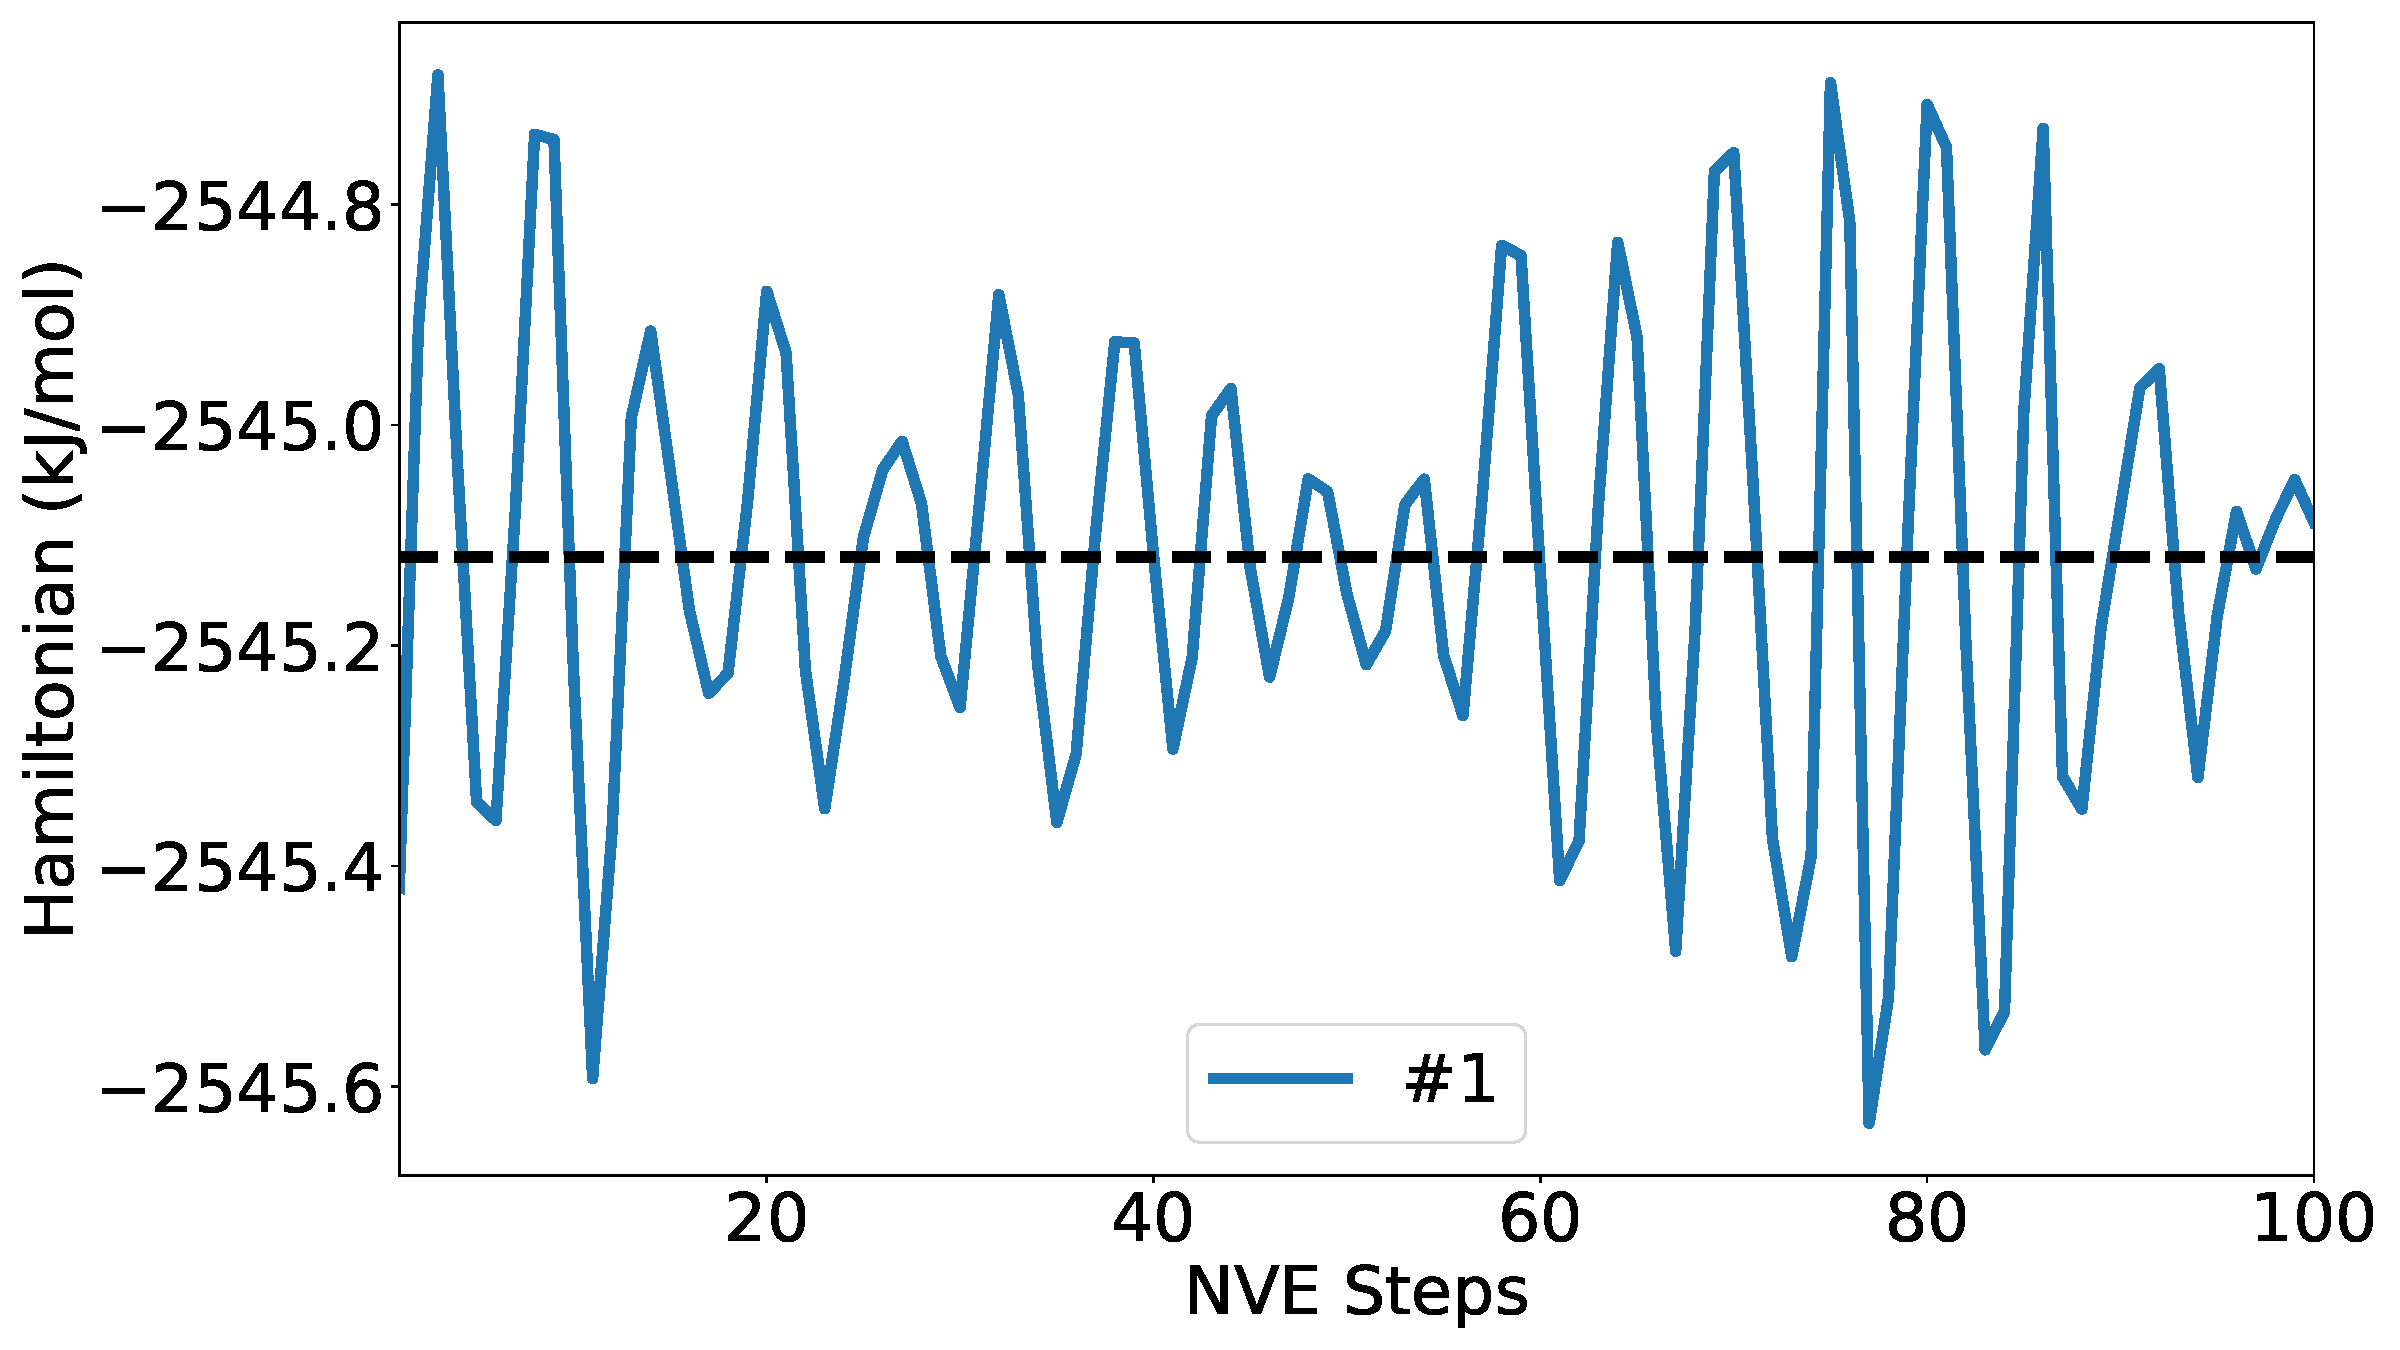
\includegraphics[width=\linewidth]{figs/drift1.pdf}
\end{subfigure}
\begin{subfigure}{0.48\textwidth}
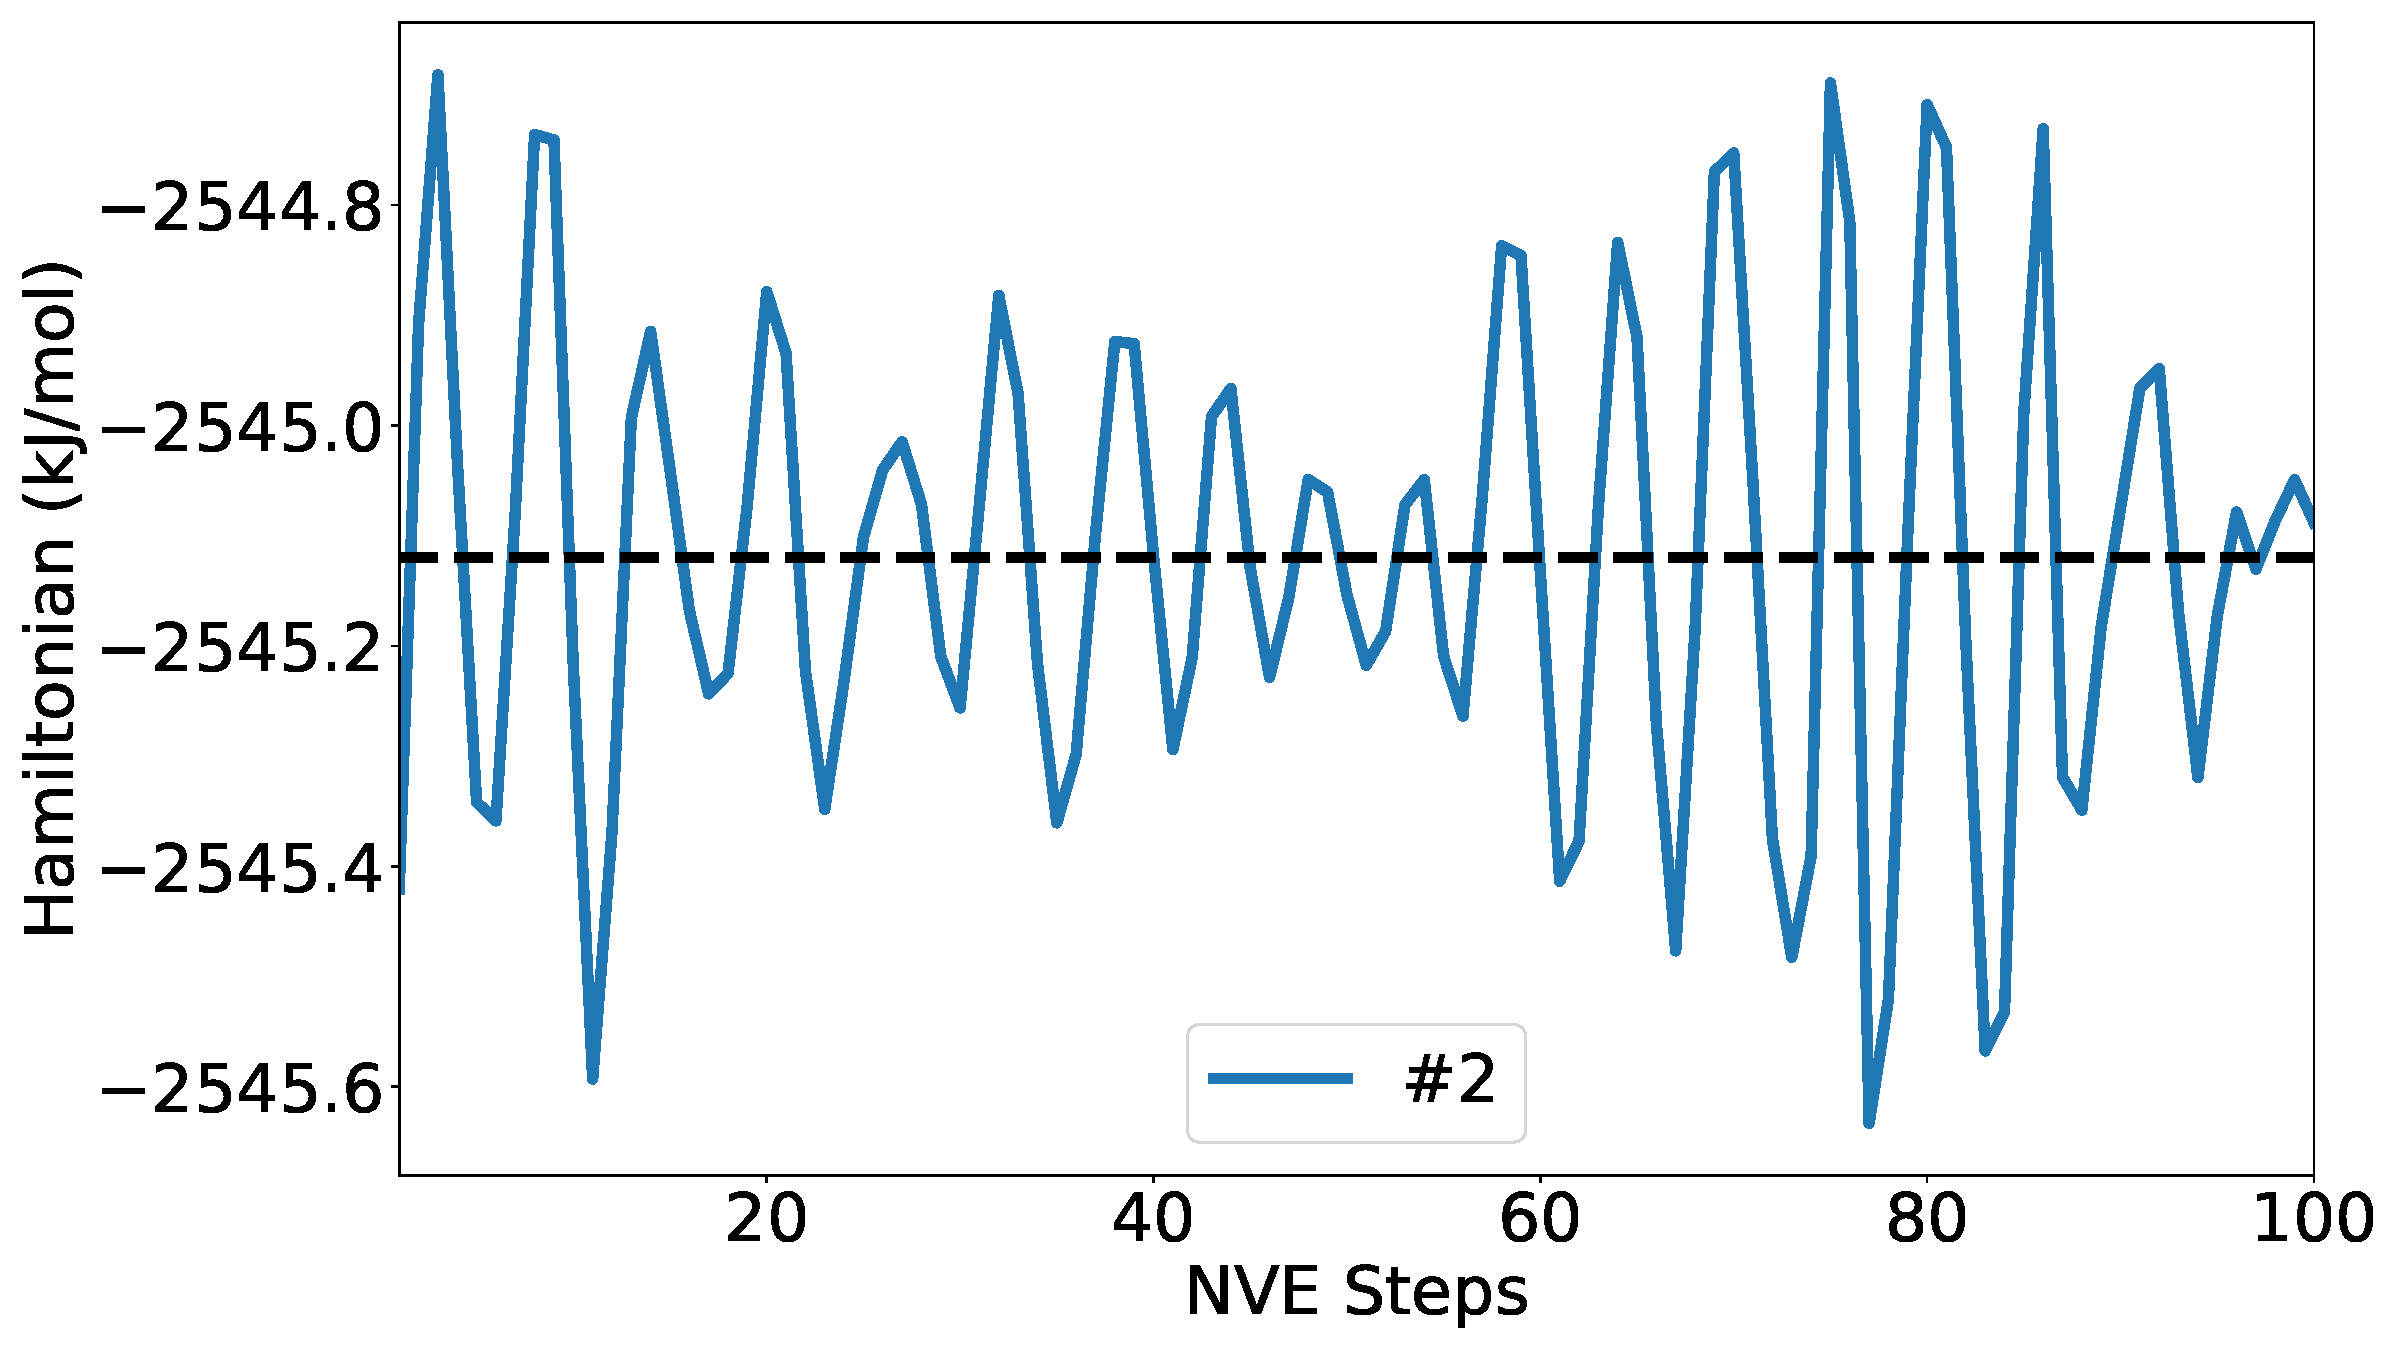
\includegraphics[width=\linewidth]{figs/drift2.pdf}
\end{subfigure}
\\
\begin{subfigure}{0.48\textwidth}
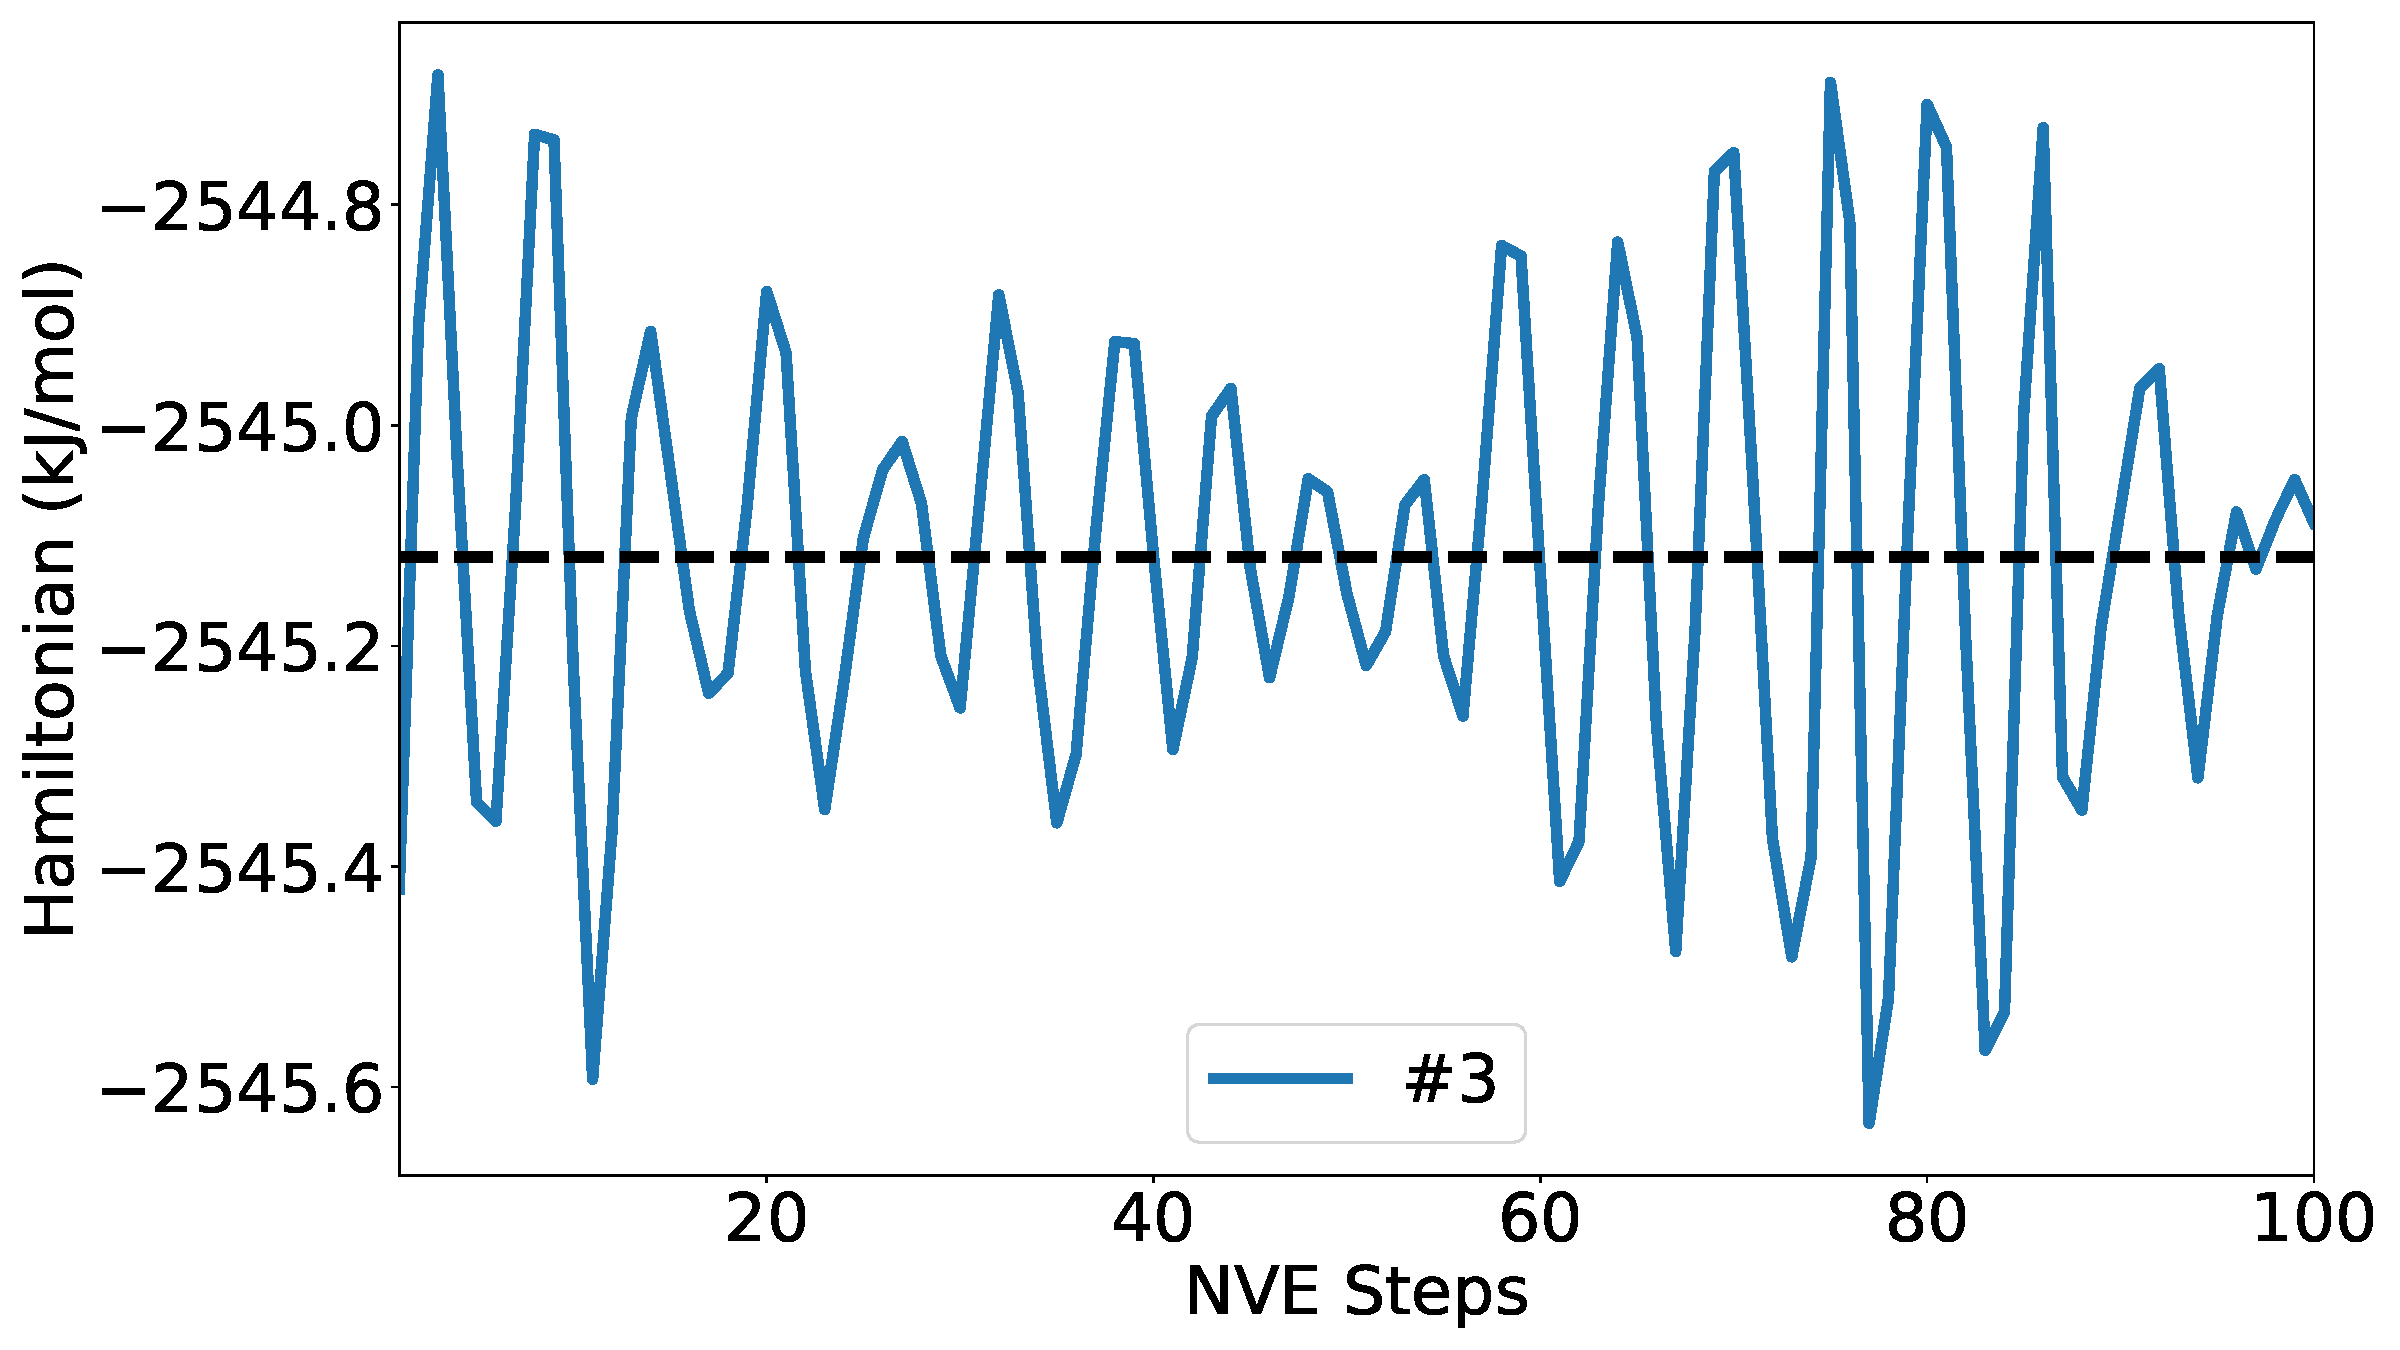
\includegraphics[width=\linewidth]{figs/drift3.pdf}
\end{subfigure}
\begin{subfigure}{0.48\textwidth}
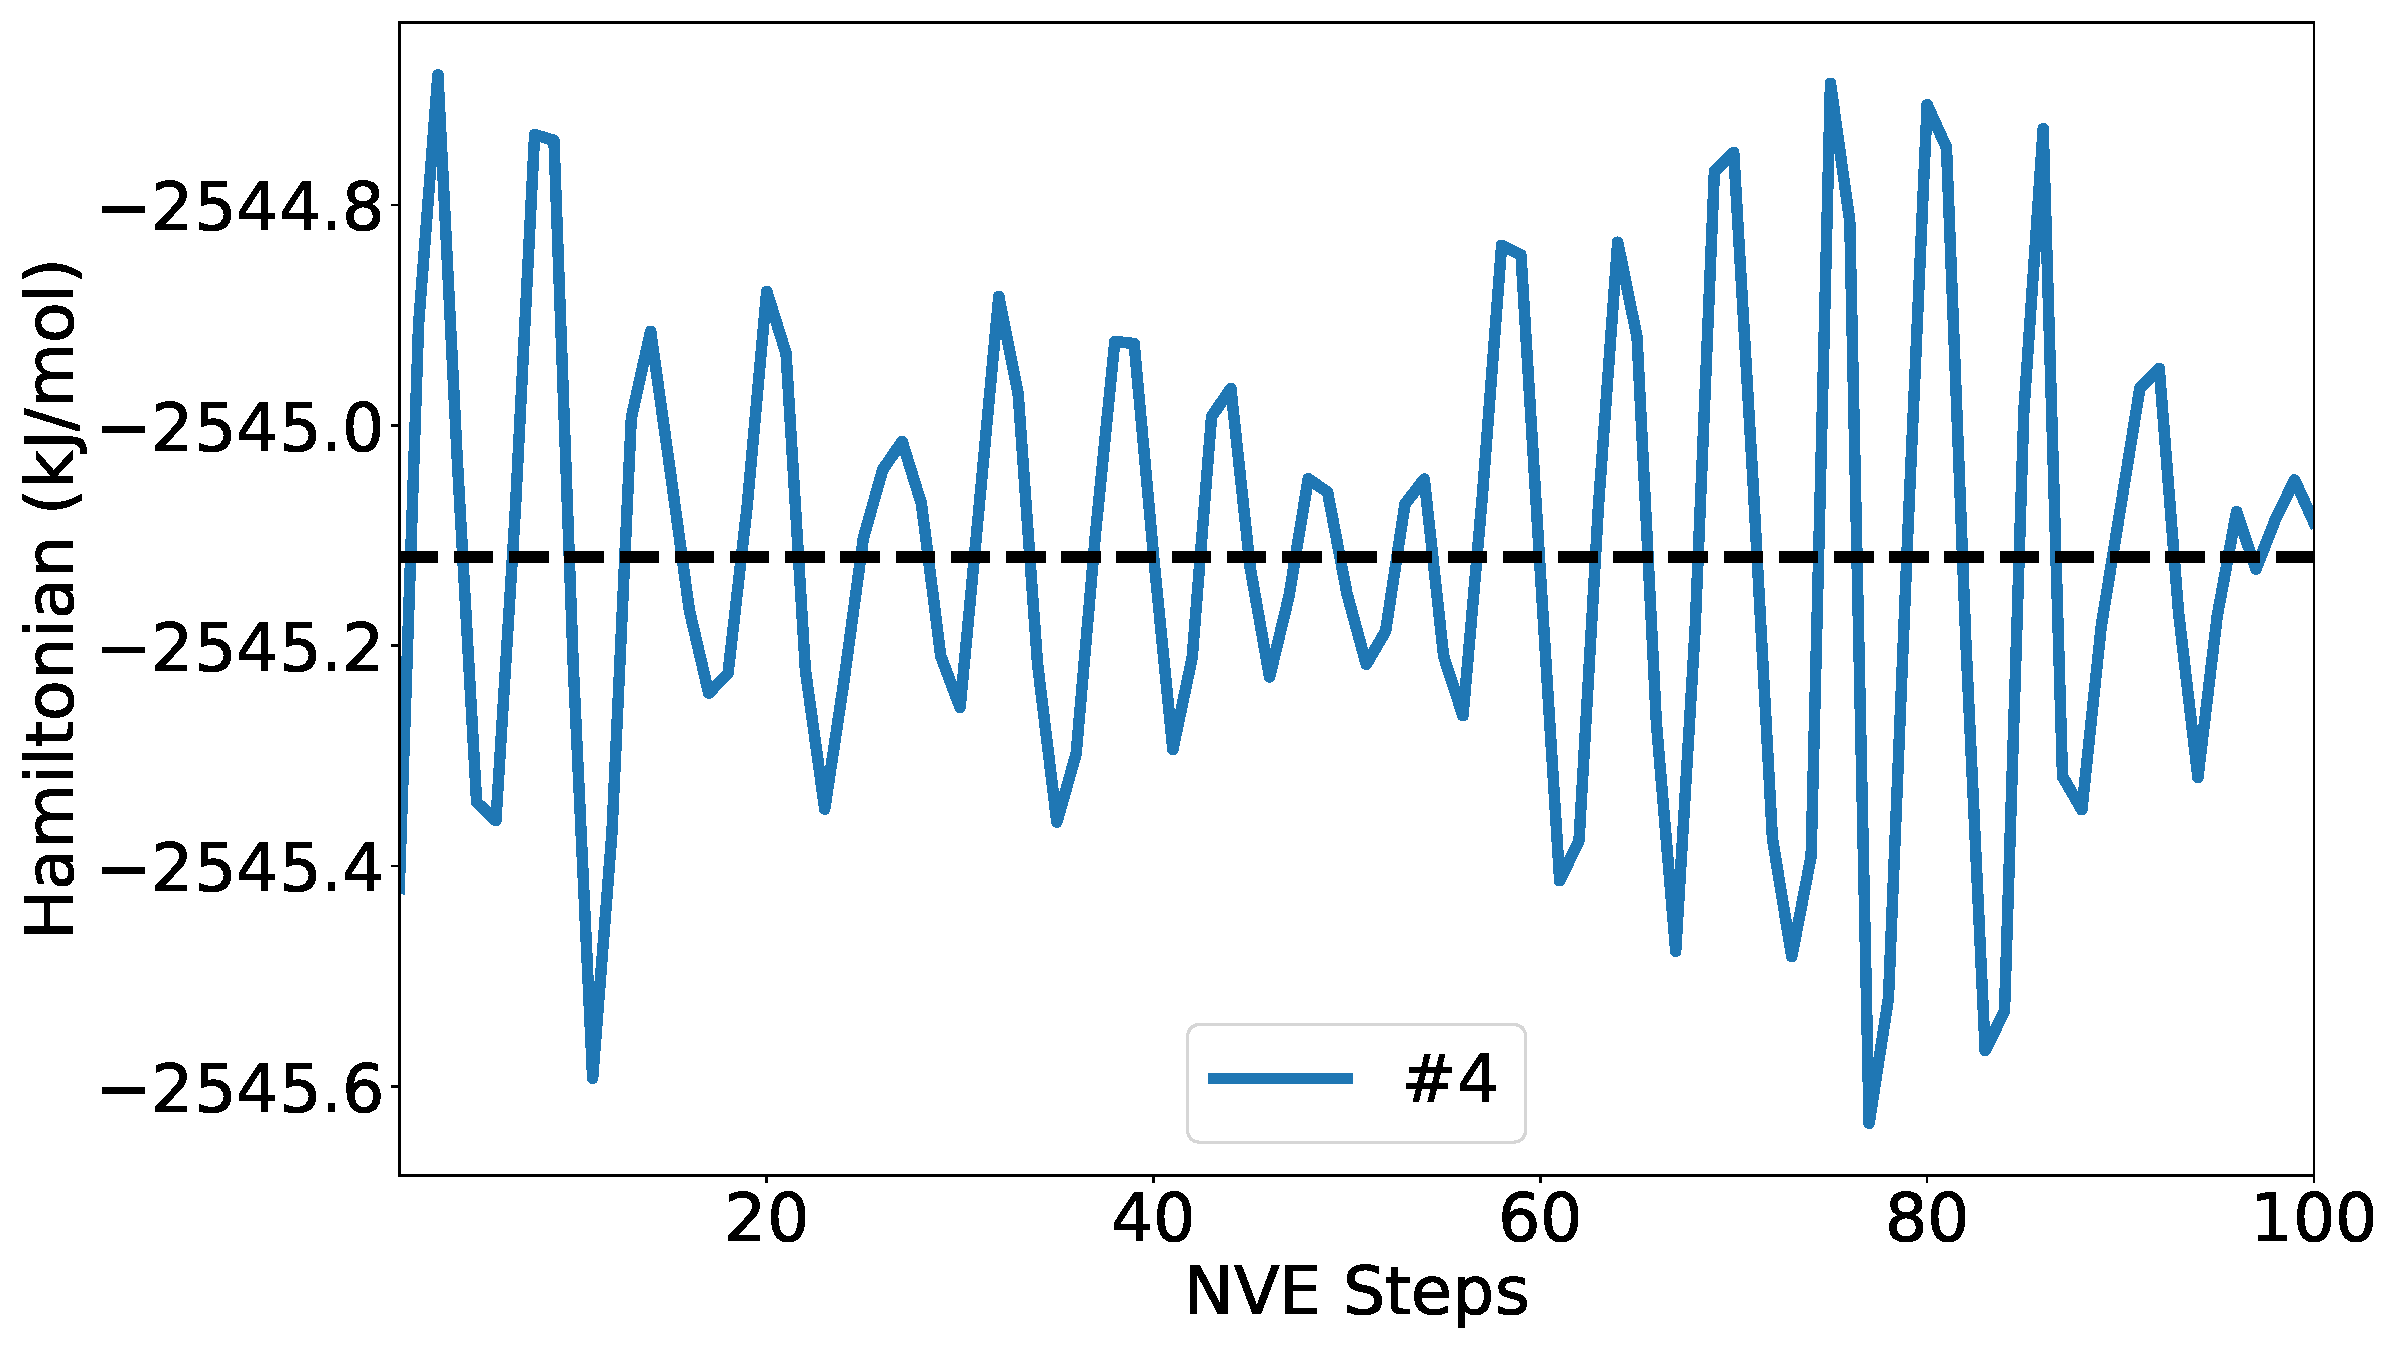
\includegraphics[width=\linewidth]{figs/drift4.pdf}
\end{subfigure}
\\
\begin{subfigure}{0.48\textwidth}
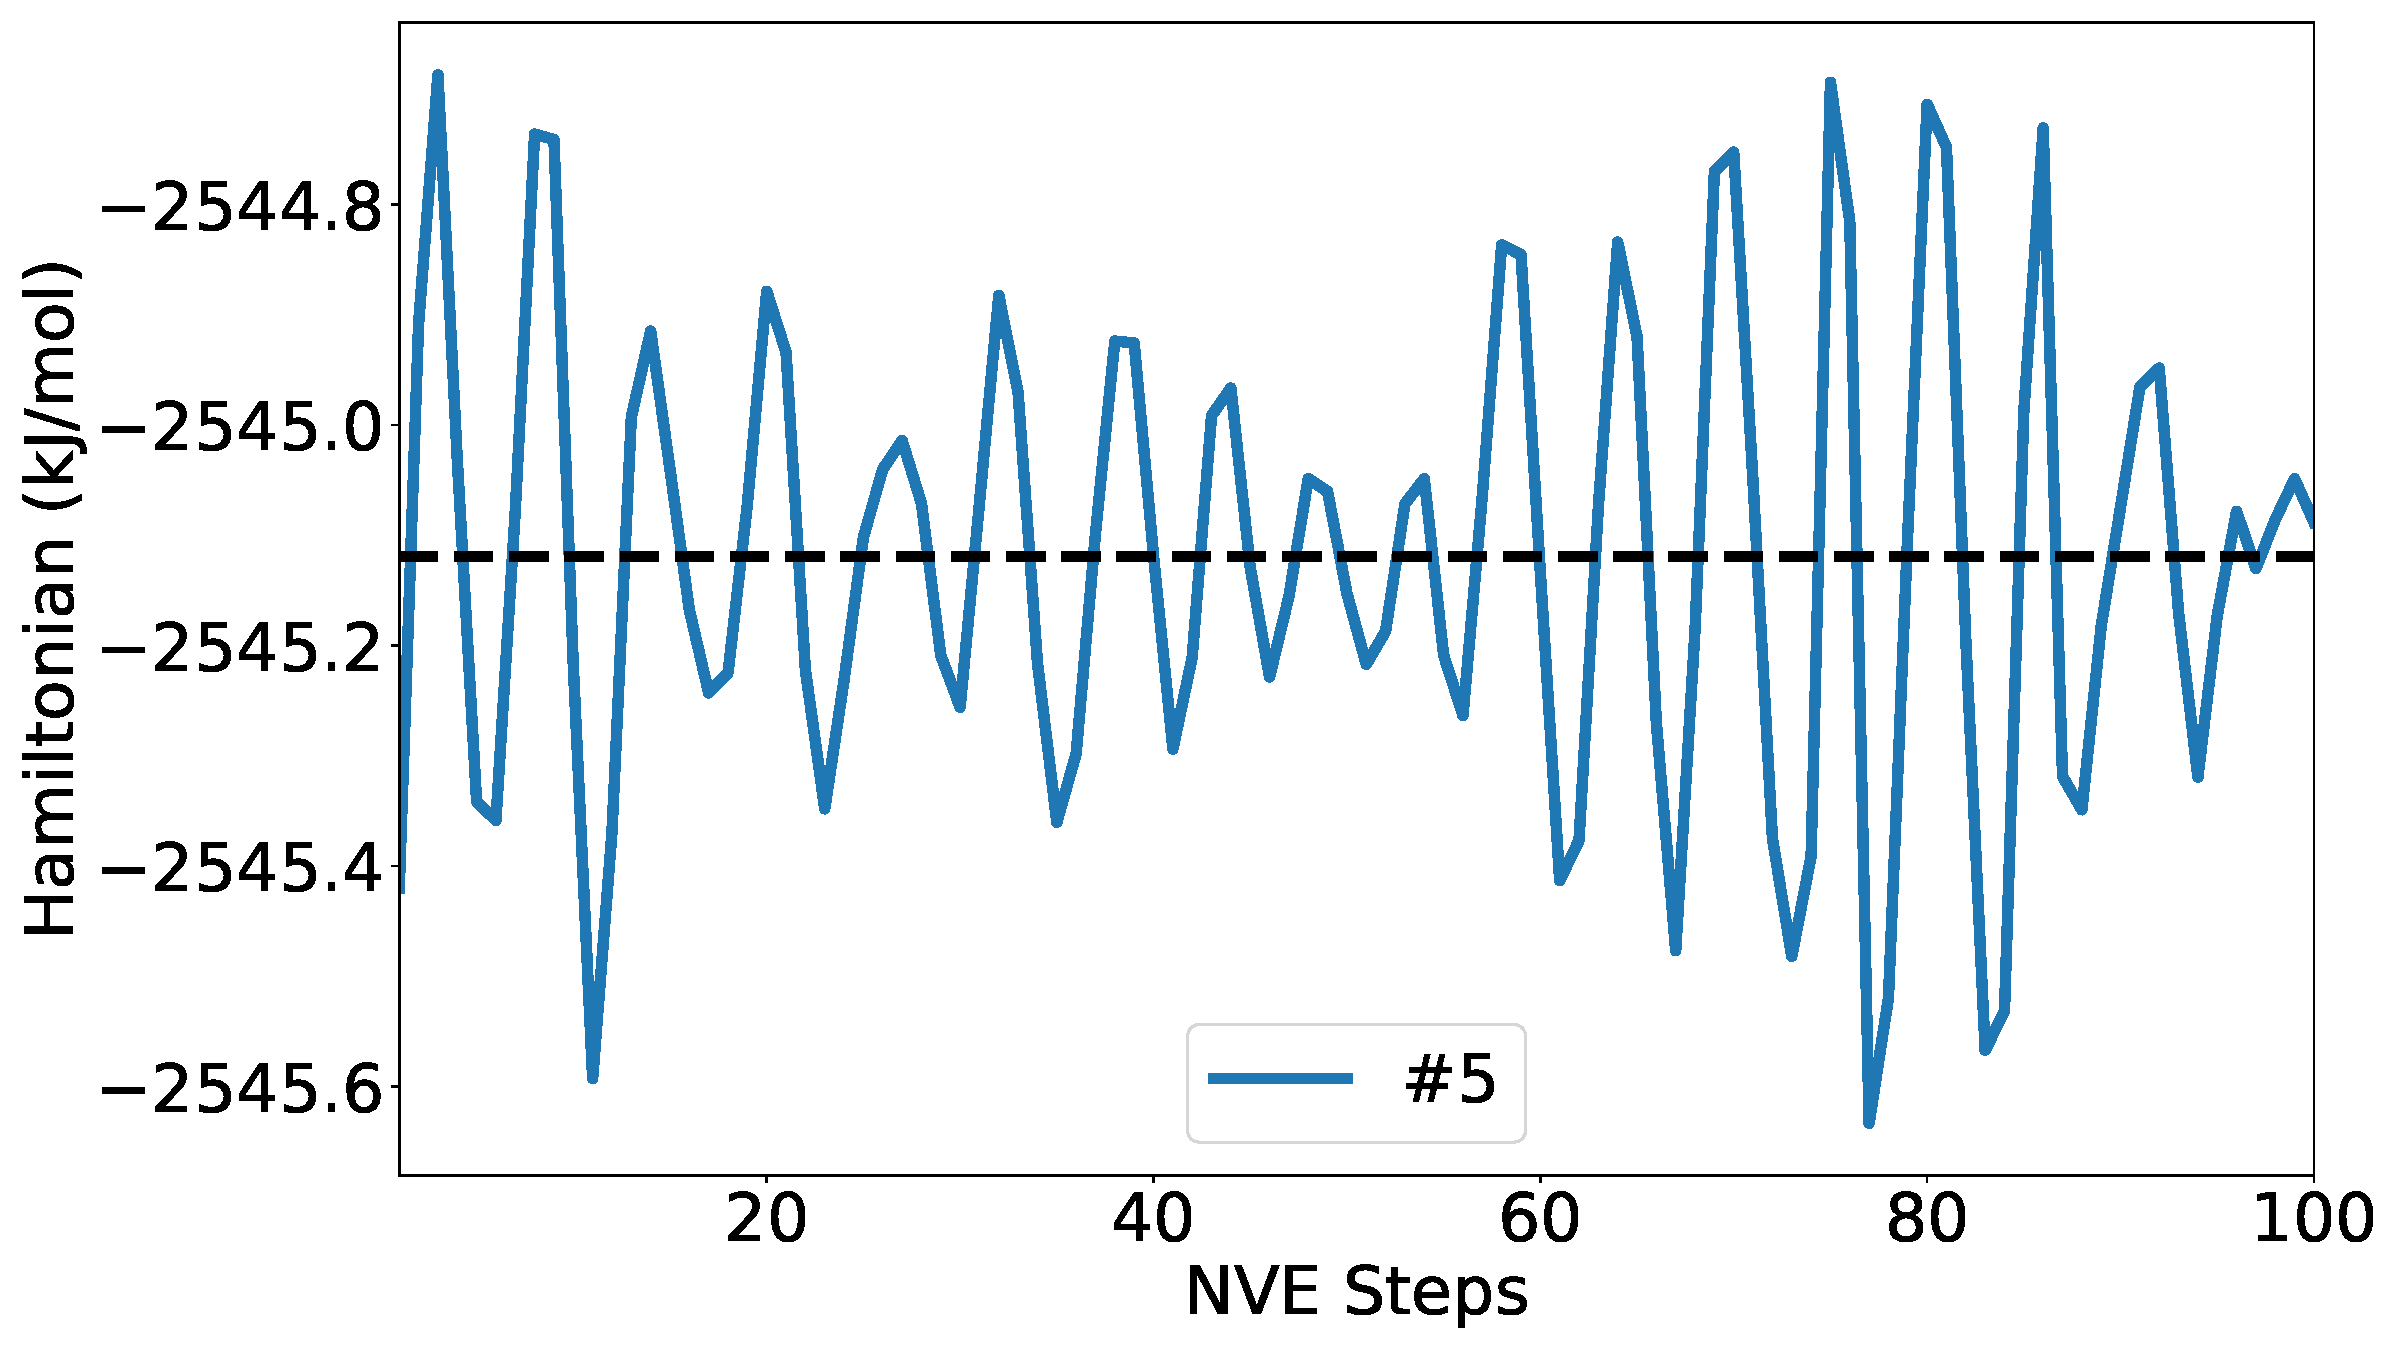
\includegraphics[width=\linewidth]{figs/drift5.pdf}
\end{subfigure}
\begin{subfigure}{0.48\textwidth}
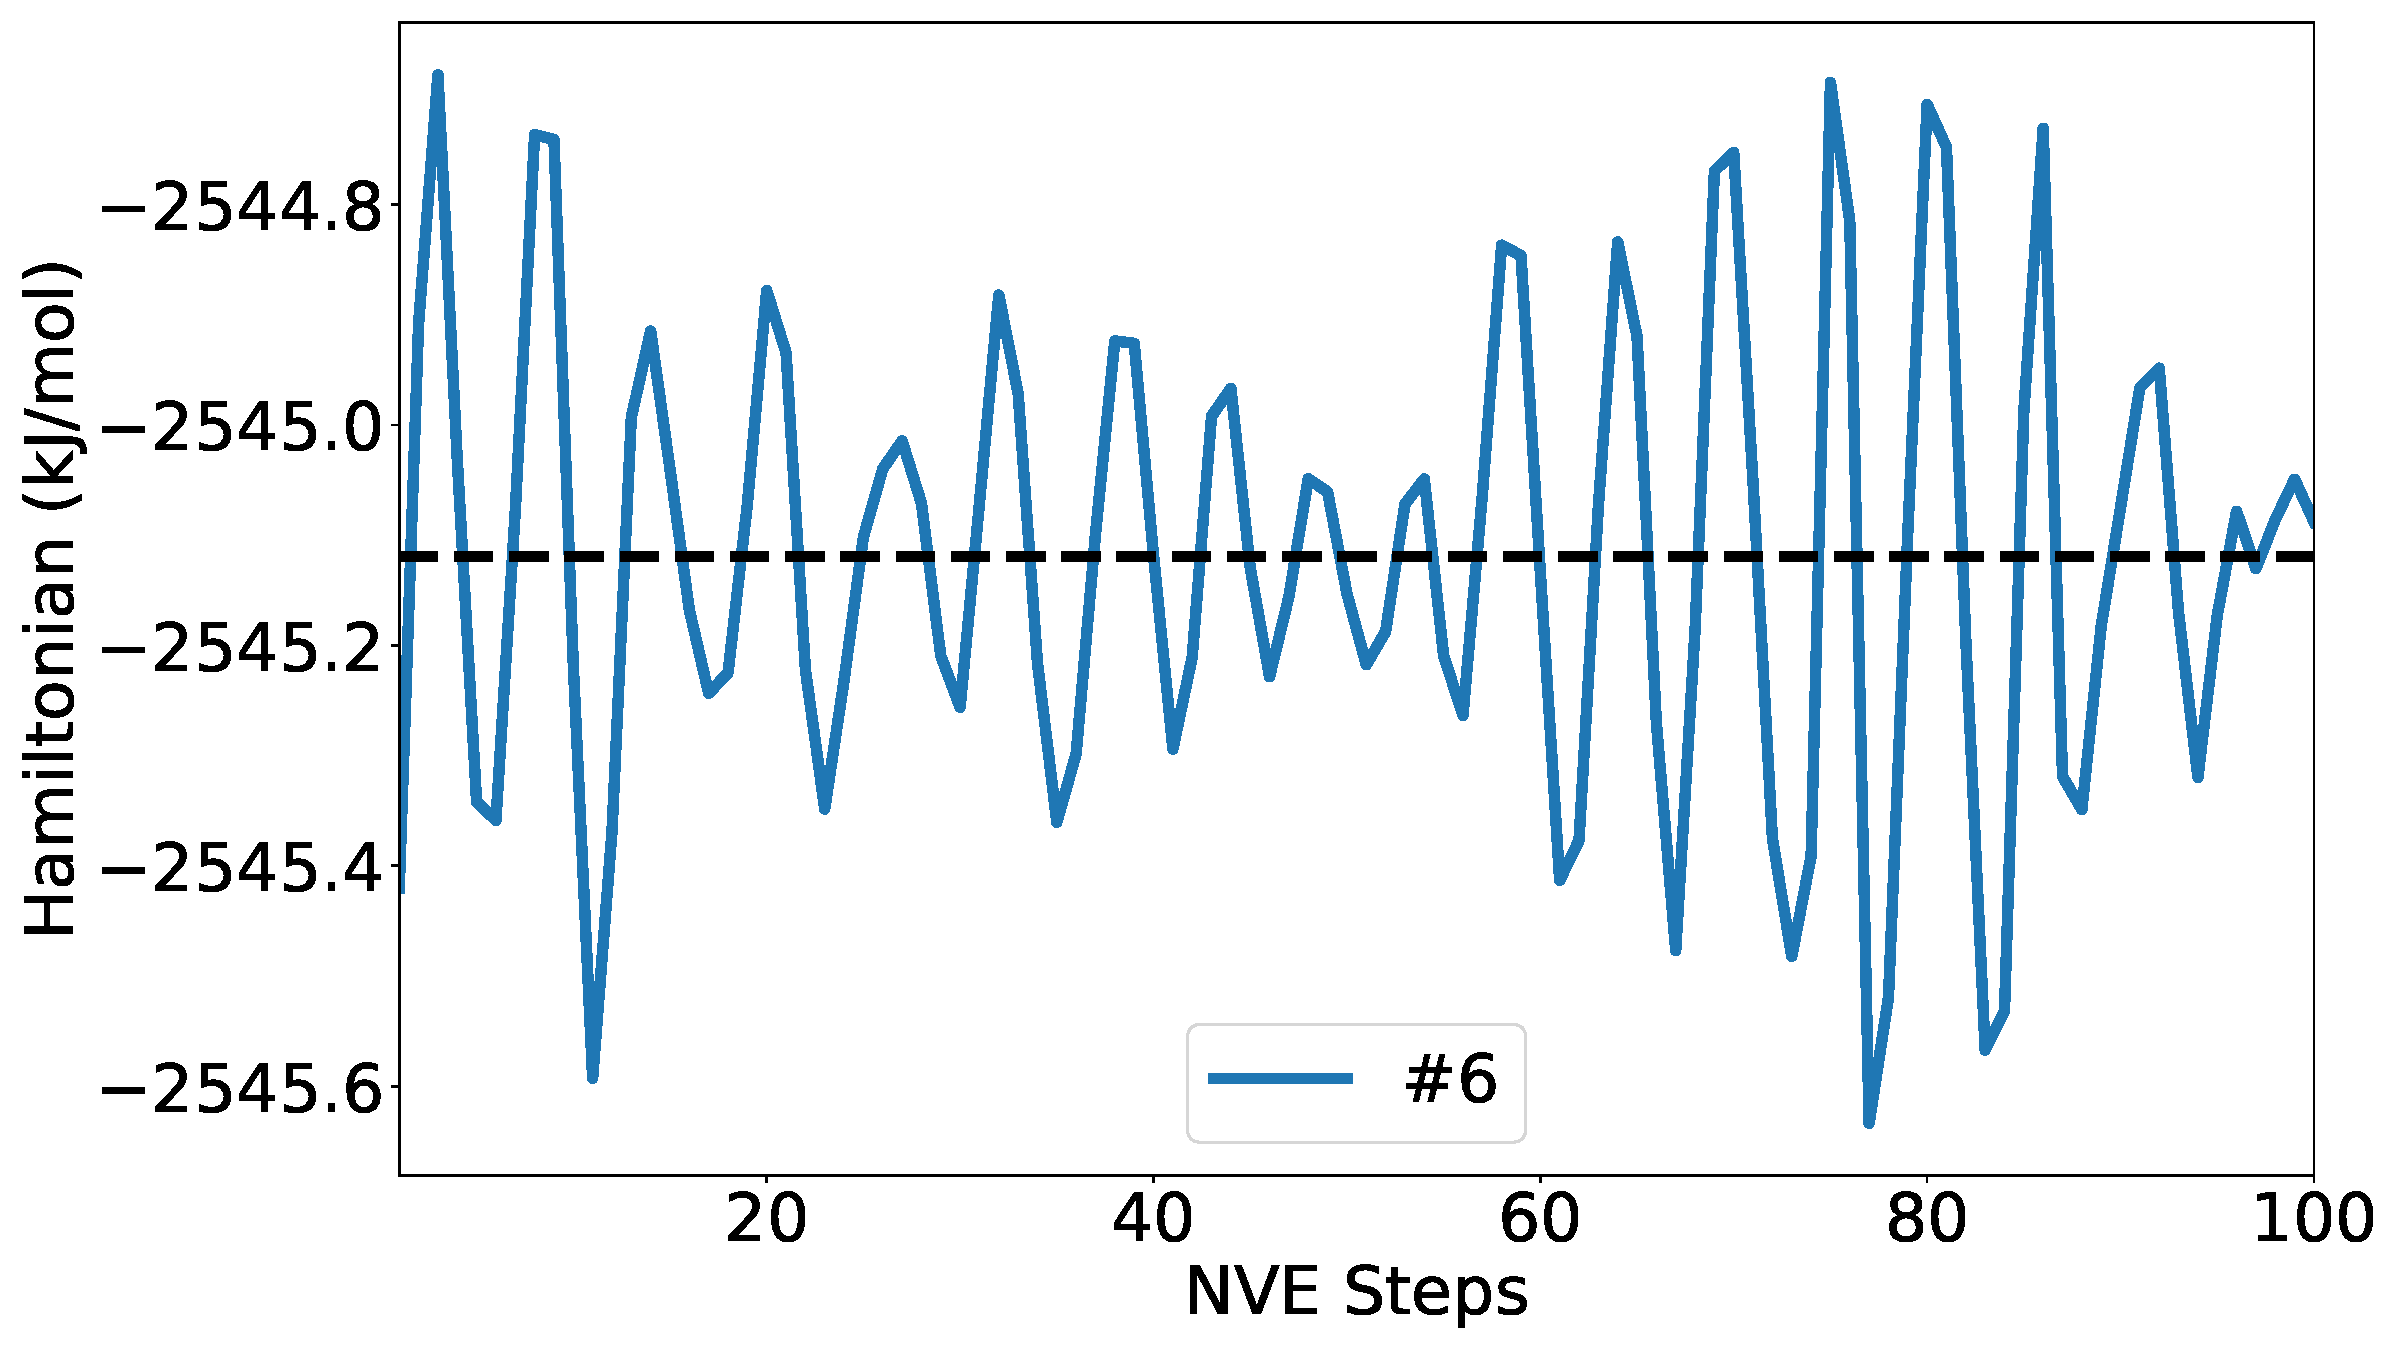
\includegraphics[width=\linewidth]{figs/drift6.pdf}
\end{subfigure}
\\
\begin{subfigure}{0.48\textwidth}
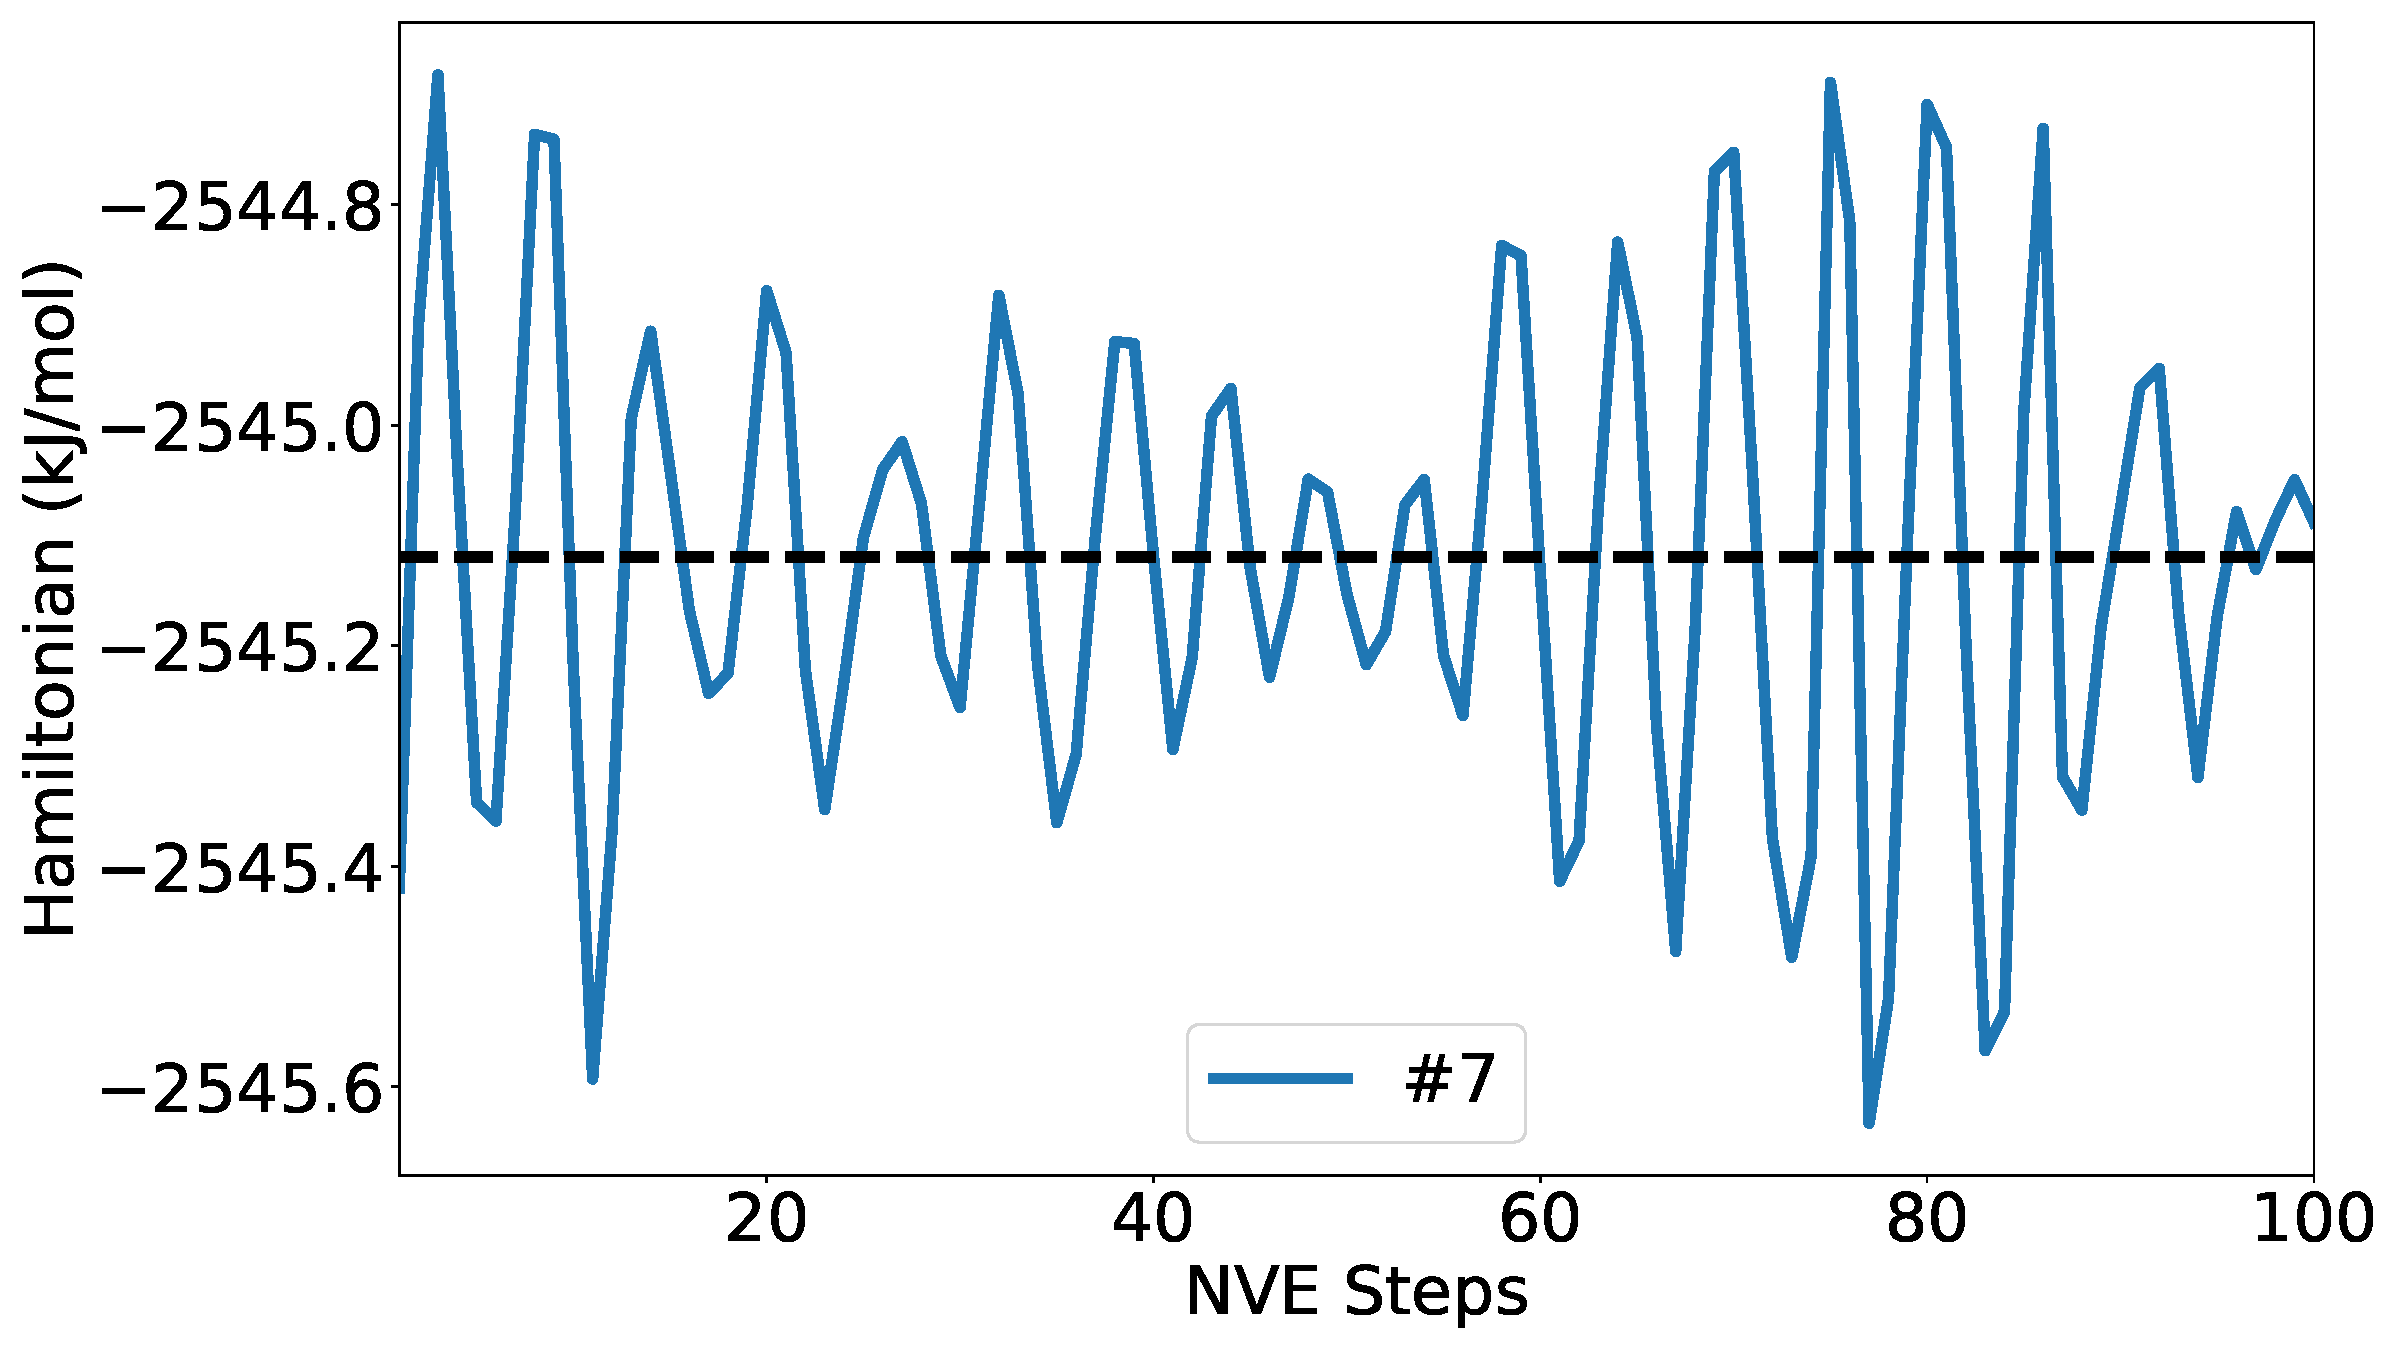
\includegraphics[width=\linewidth]{figs/drift7.pdf}
\end{subfigure}
\begin{subfigure}{0.48\textwidth}
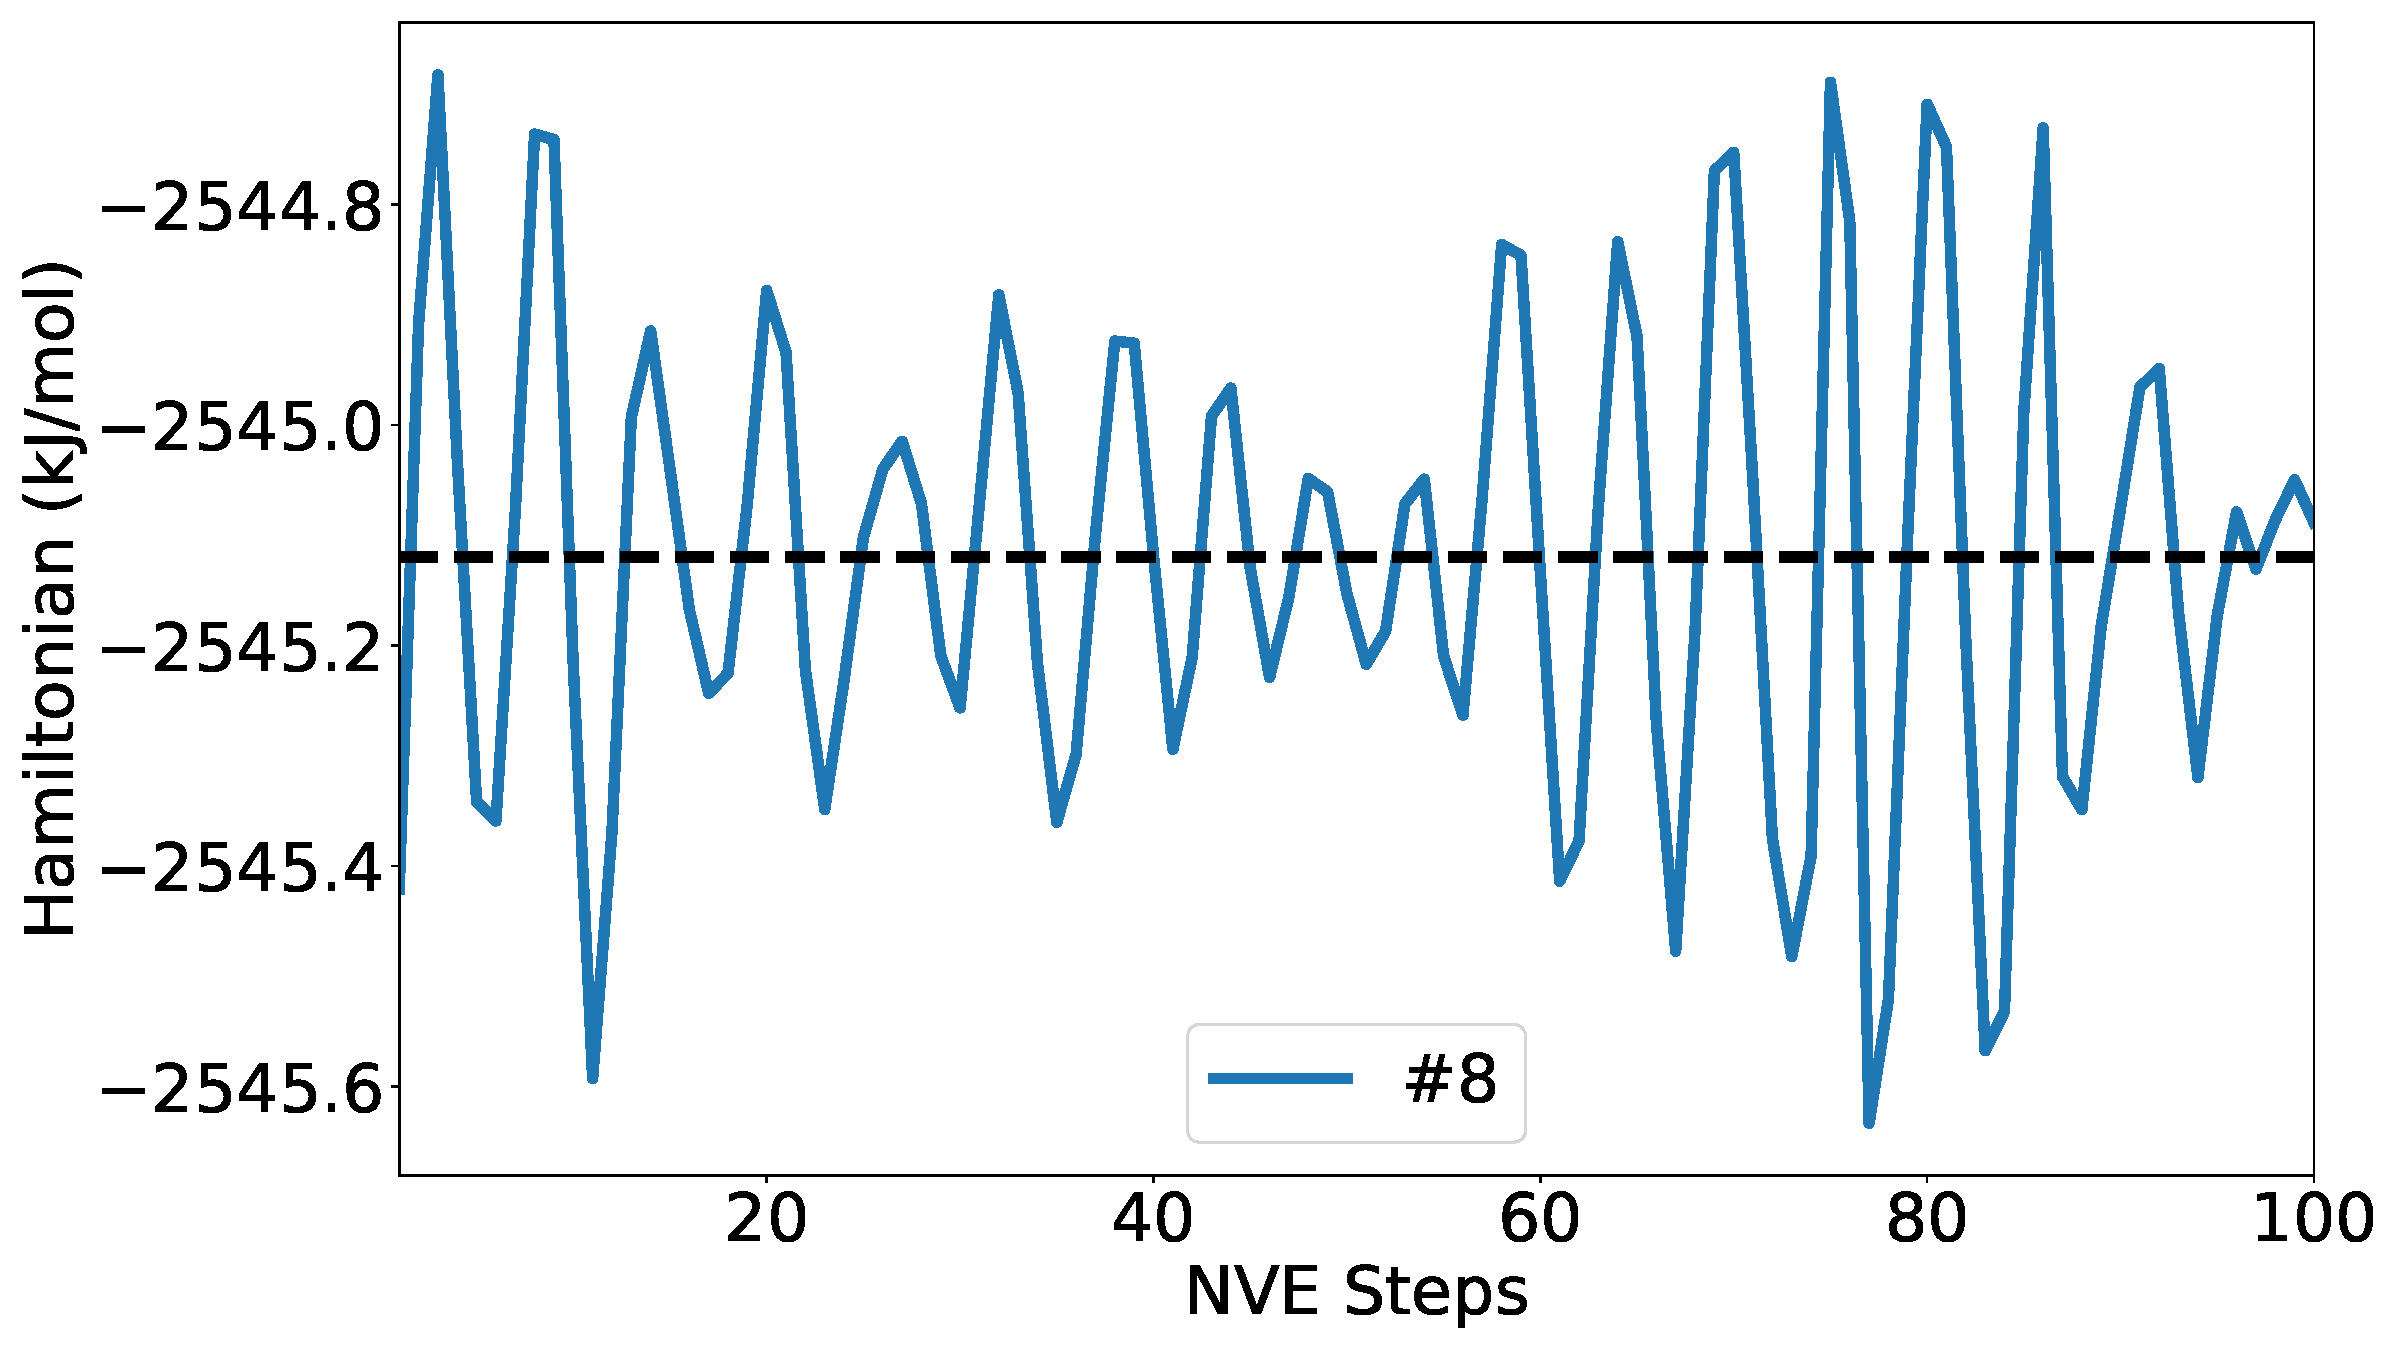
\includegraphics[width=\linewidth]{figs/drift8.pdf}
\end{subfigure}
\caption{Evolution of system Hamiltonians
over 100 time-steps for different deployment strategies.
Each subfigure corresponds to a specific strategy
as detailed in Table~\ref{tb:deploy8}.
Dashed lines indicate the mean Hamiltonian value.}\label{fig:drift}
\end{figure*}

\else\fi

\textbf{Trajectory Convergence}
Figure~\ref{fig:convergence} depicts the differences per time-step
in potential energy ($U$), kinetic energy ($K$), and Hamiltonian ($H$)
between the baseline and other implementations.
The energies maintained convergence throughout the 100 time-steps,
with numerical differences approaching the theoretical limit of fp32 precision
(approximately the 6th or 7th significant figure).
The spatial coordinates, recorded in the PDB format,
exhibited consistency up to three decimal places
with a maximum deviation of $0.001$~\AA{} on all trajectories.

\ifdefined\InlineFloatEnv
\begin{figure*}[htbp]
\begin{subfigure}{0.48\textwidth}
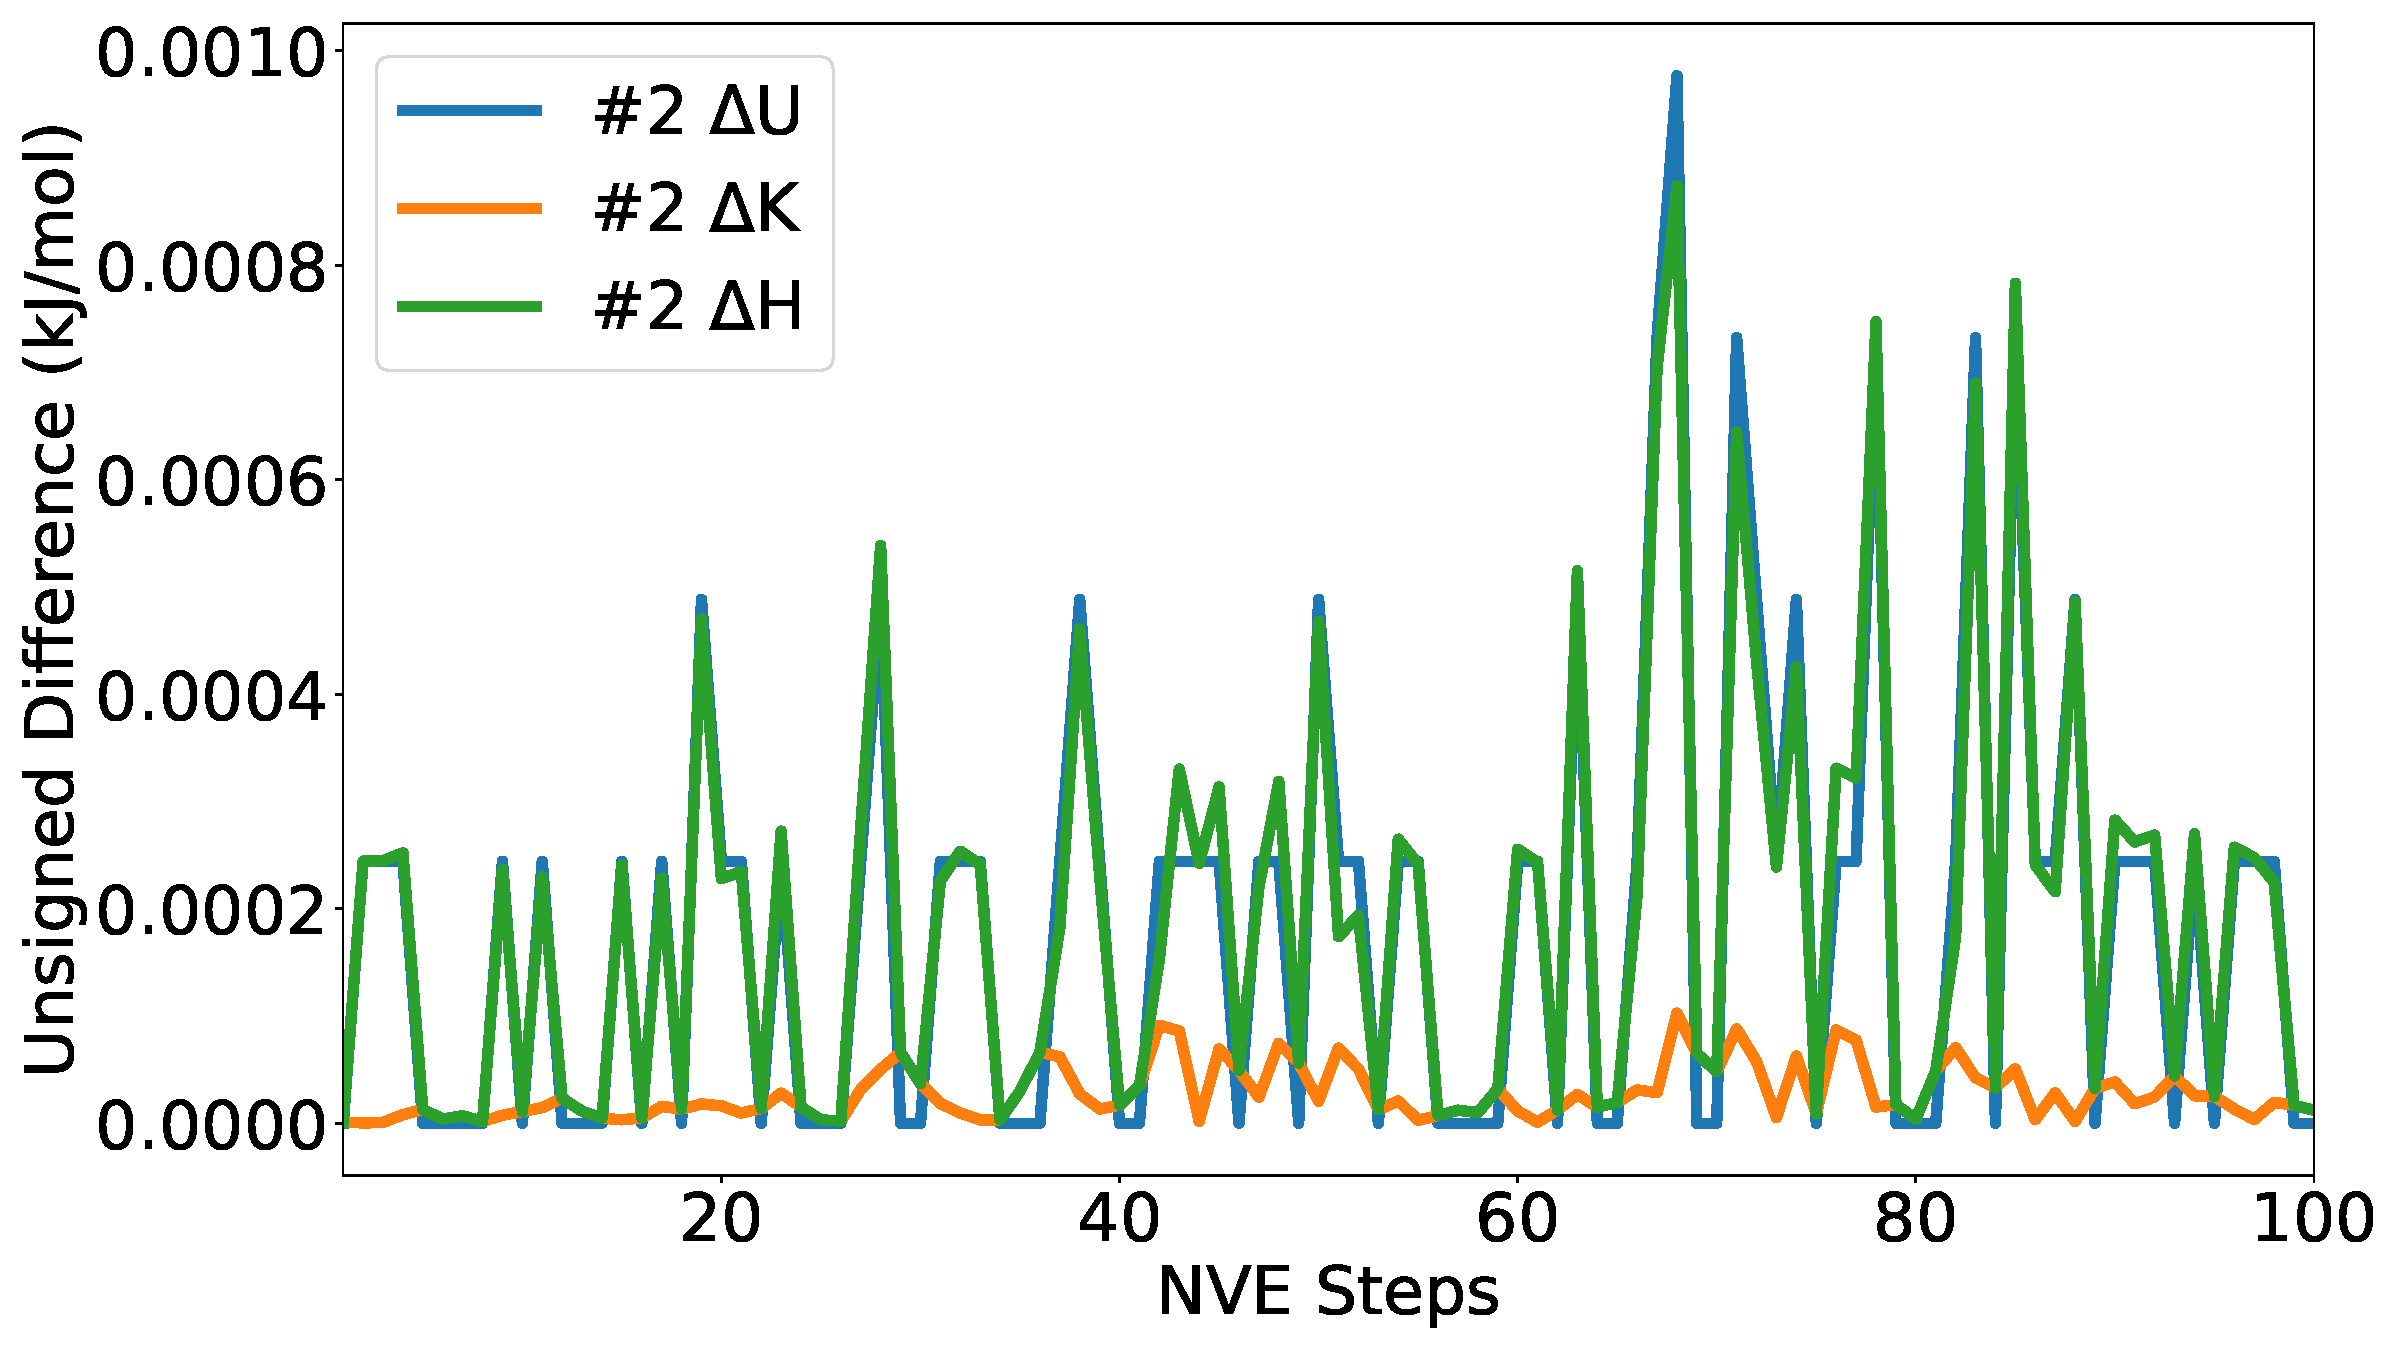
\includegraphics[width=\linewidth]{figs/div2.pdf}
\end{subfigure}
\\
\begin{subfigure}{0.48\textwidth}
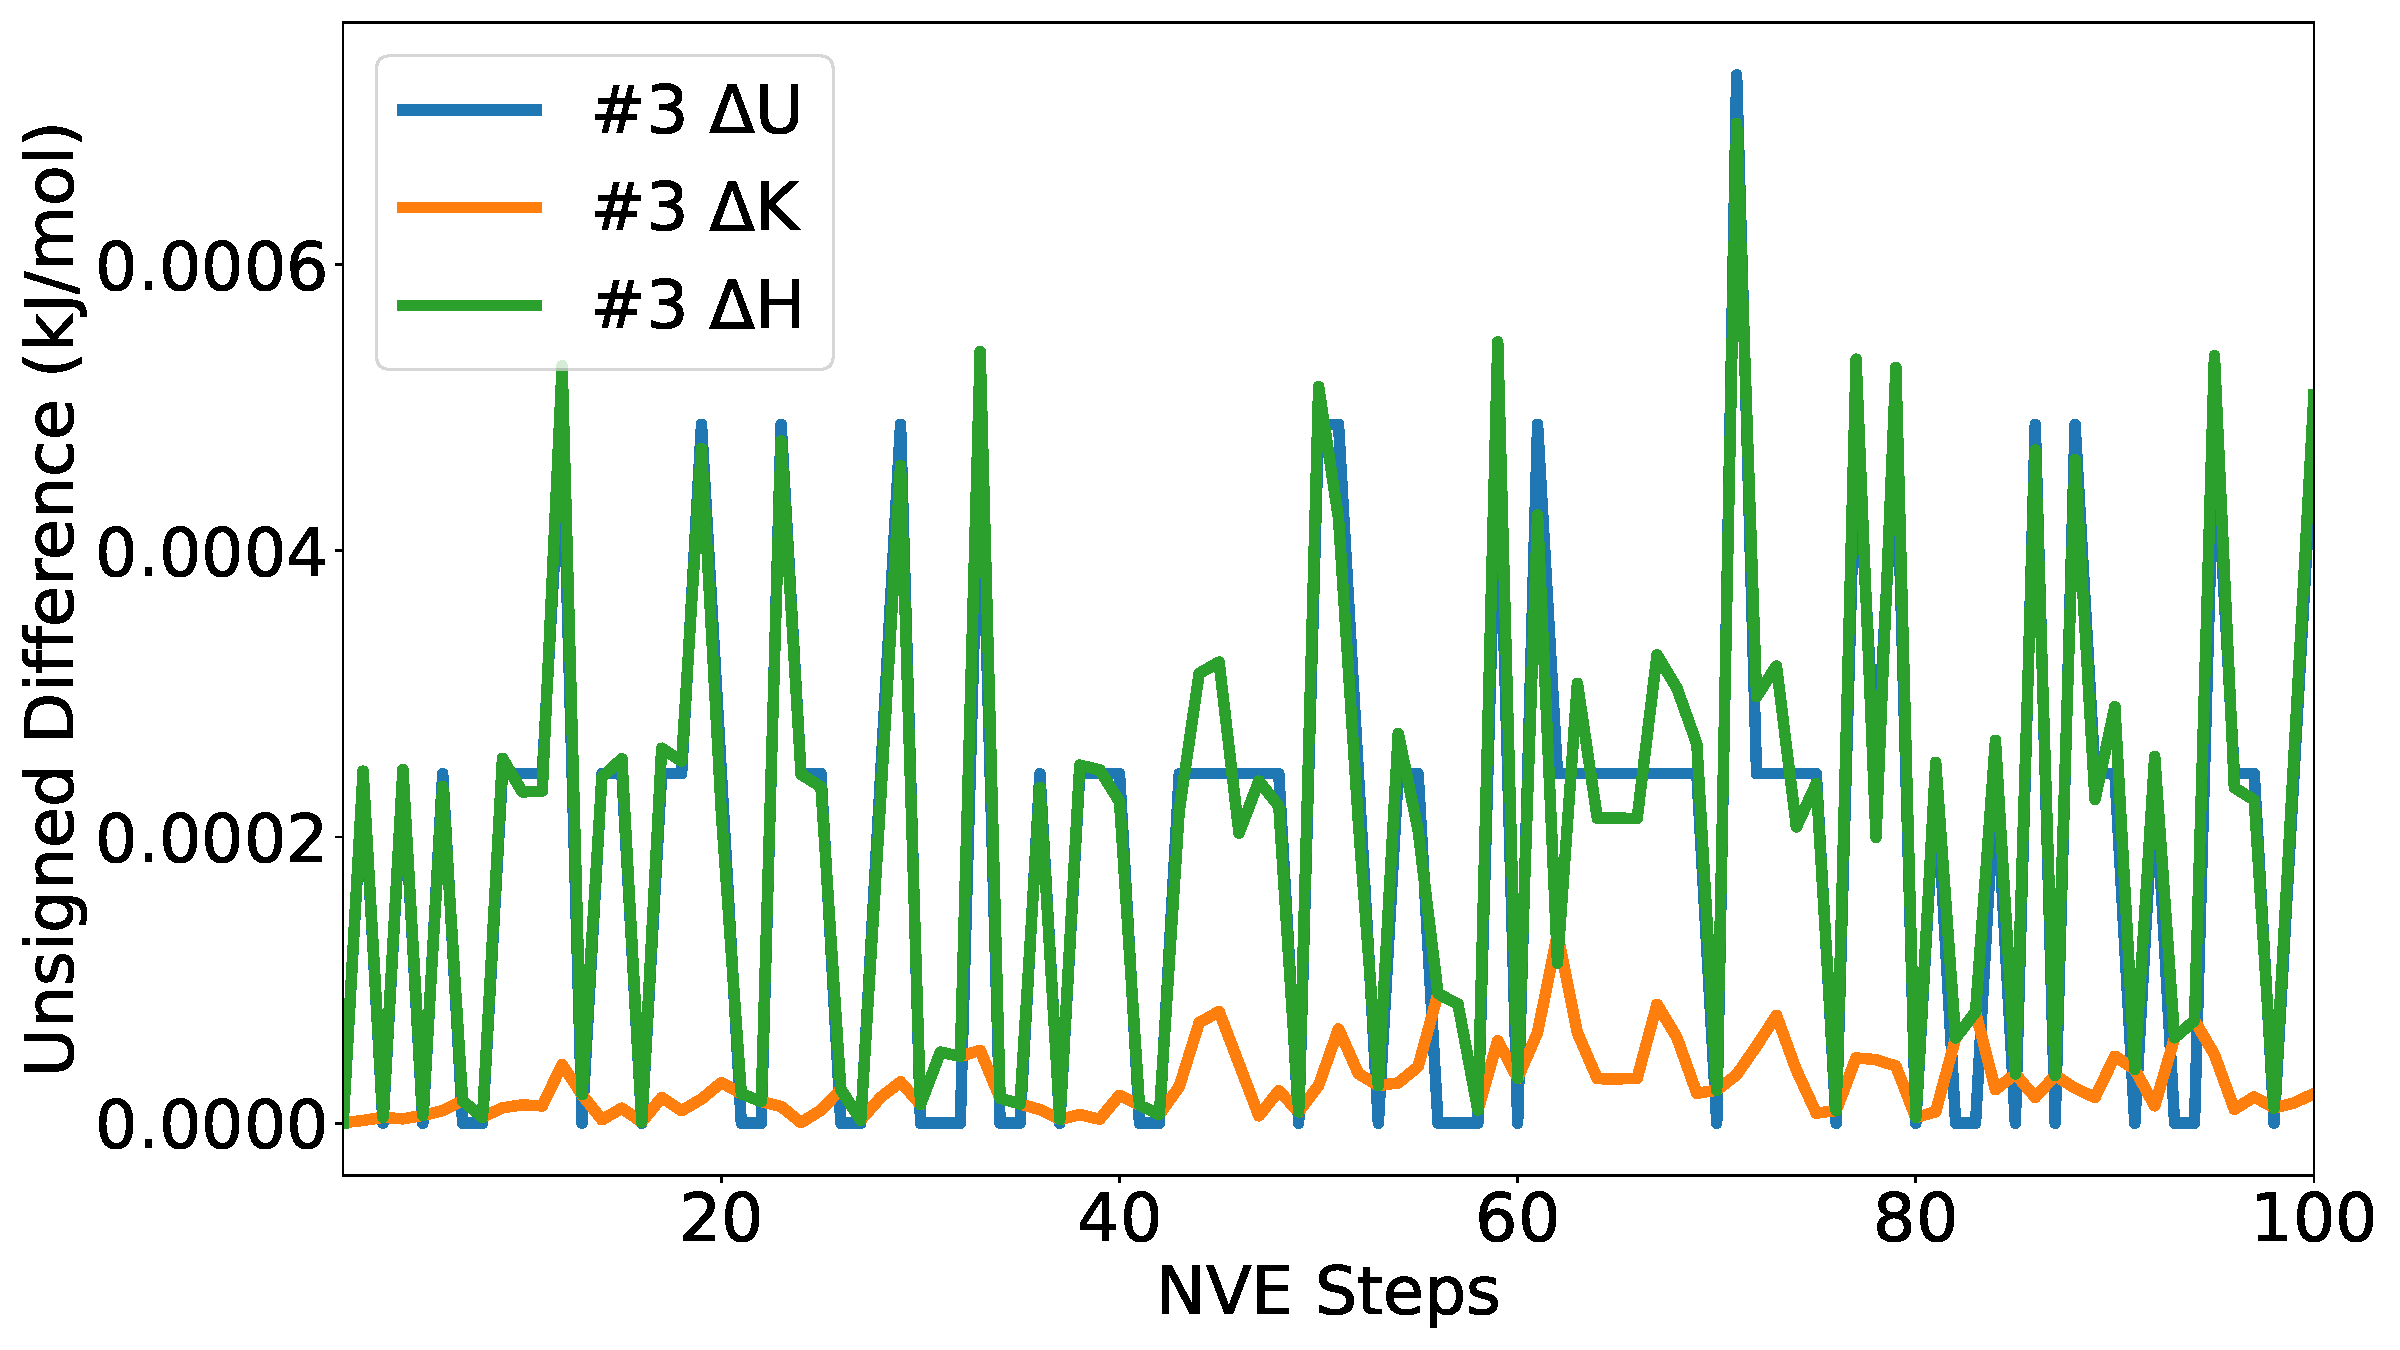
\includegraphics[width=\linewidth]{figs/div3.pdf}
\end{subfigure}
\begin{subfigure}{0.48\textwidth}
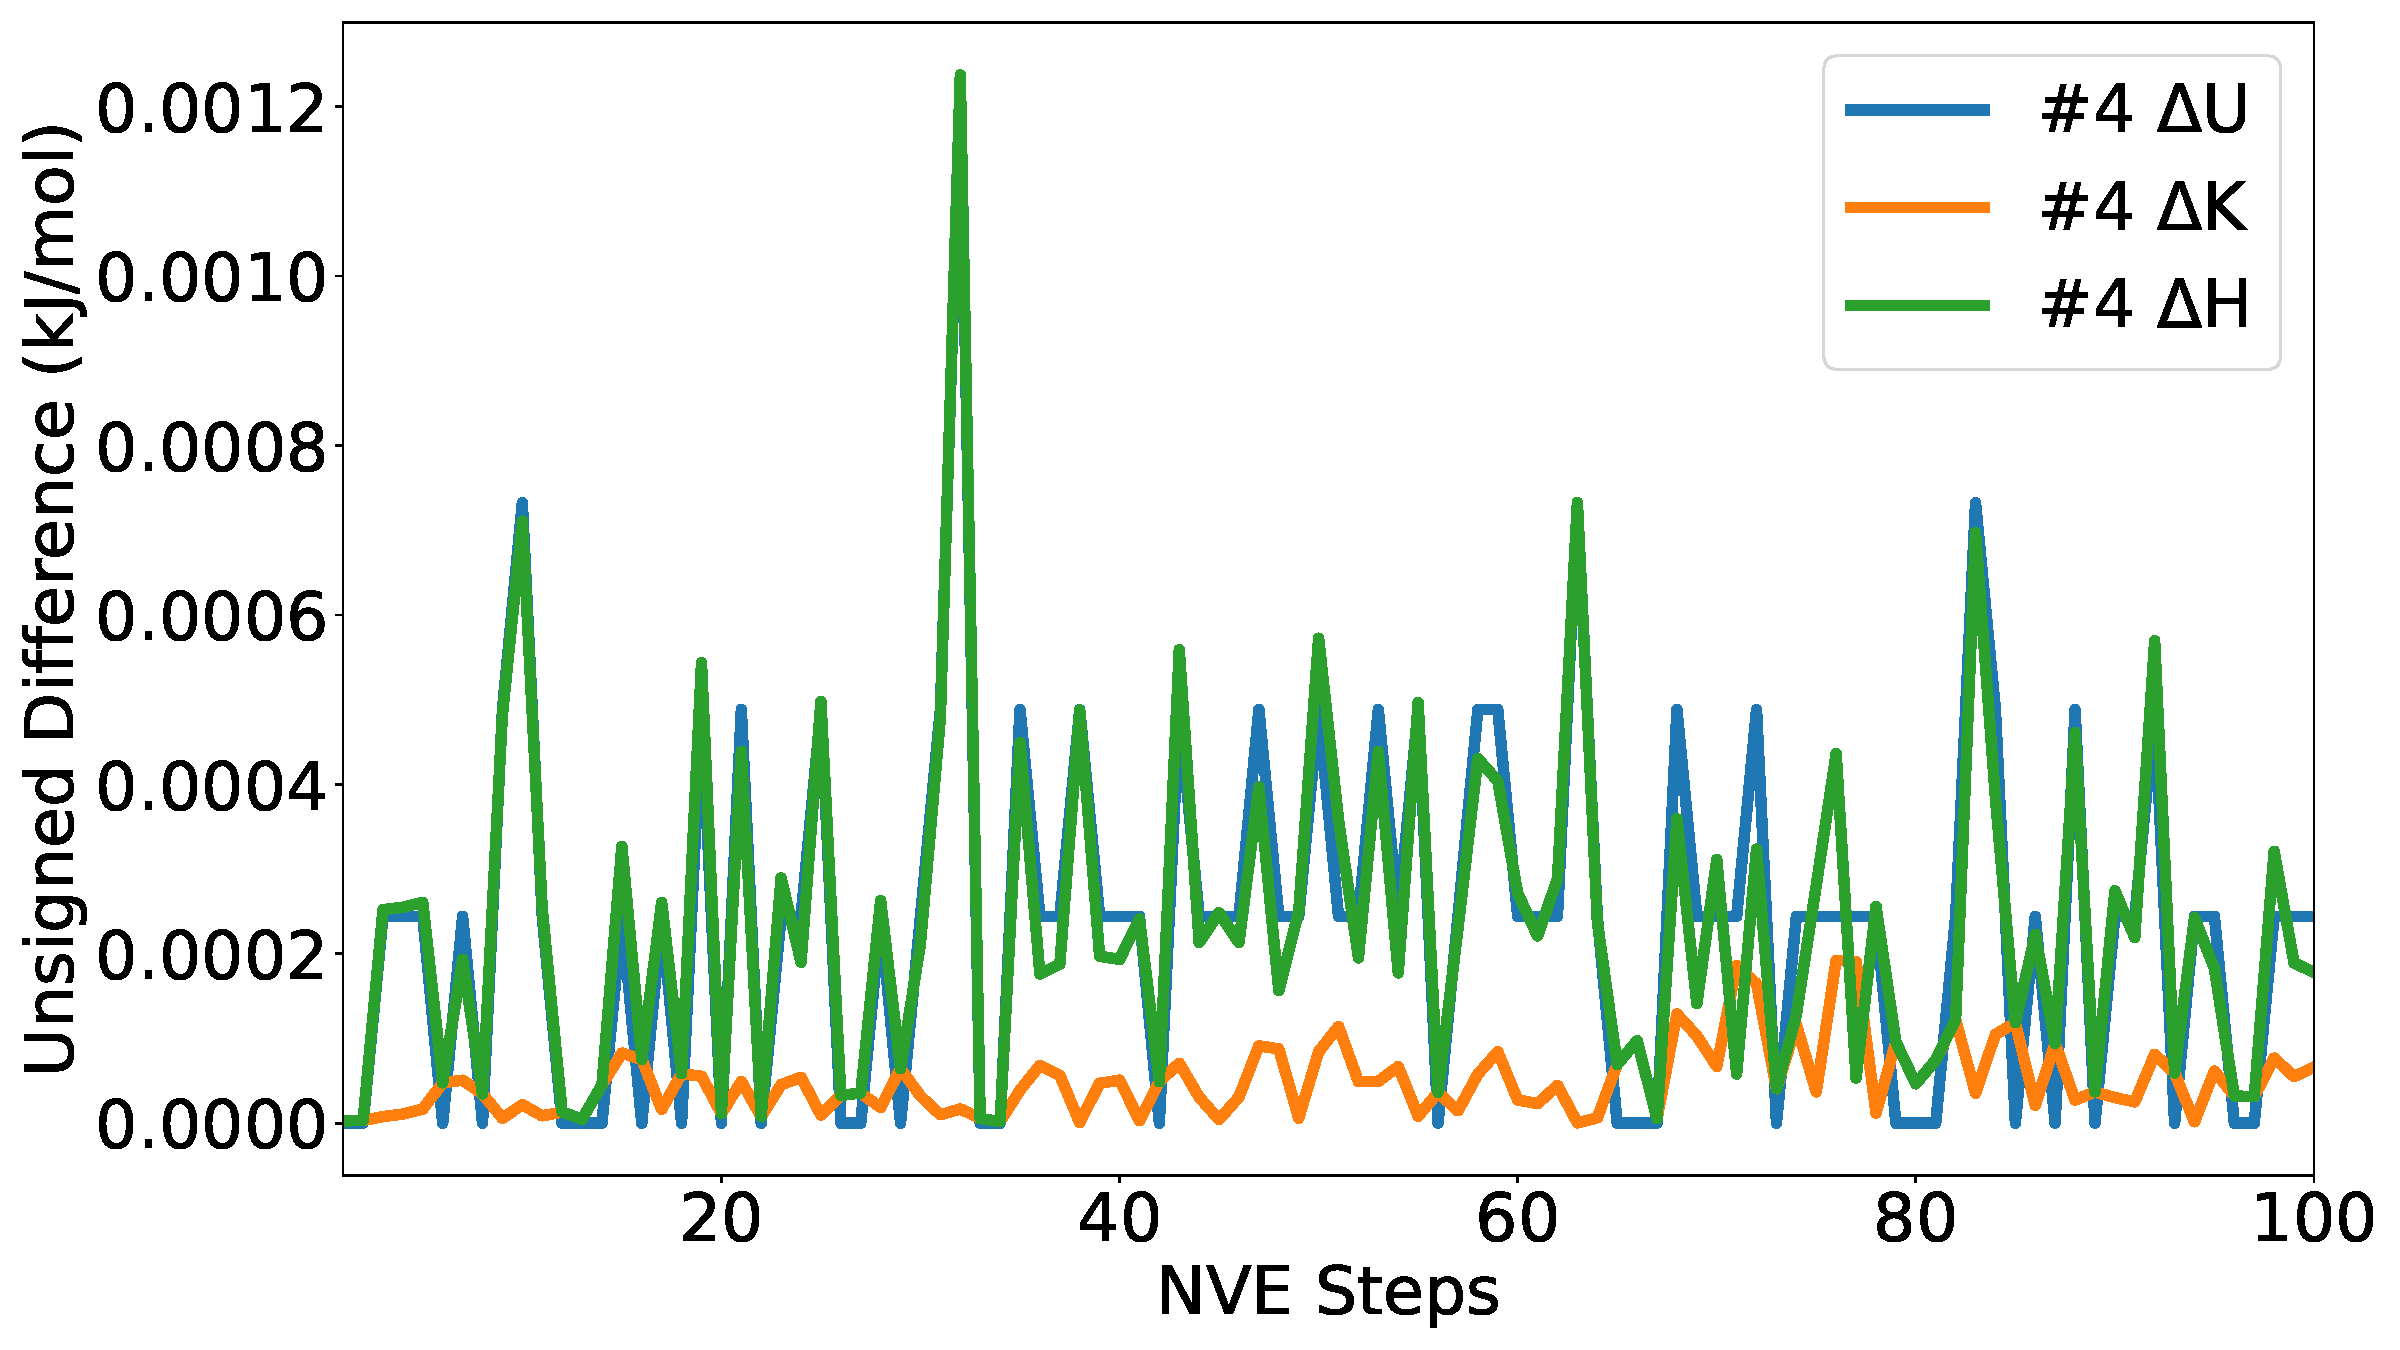
\includegraphics[width=\linewidth]{figs/div4.pdf}
\end{subfigure}
\\
\begin{subfigure}{0.48\textwidth}
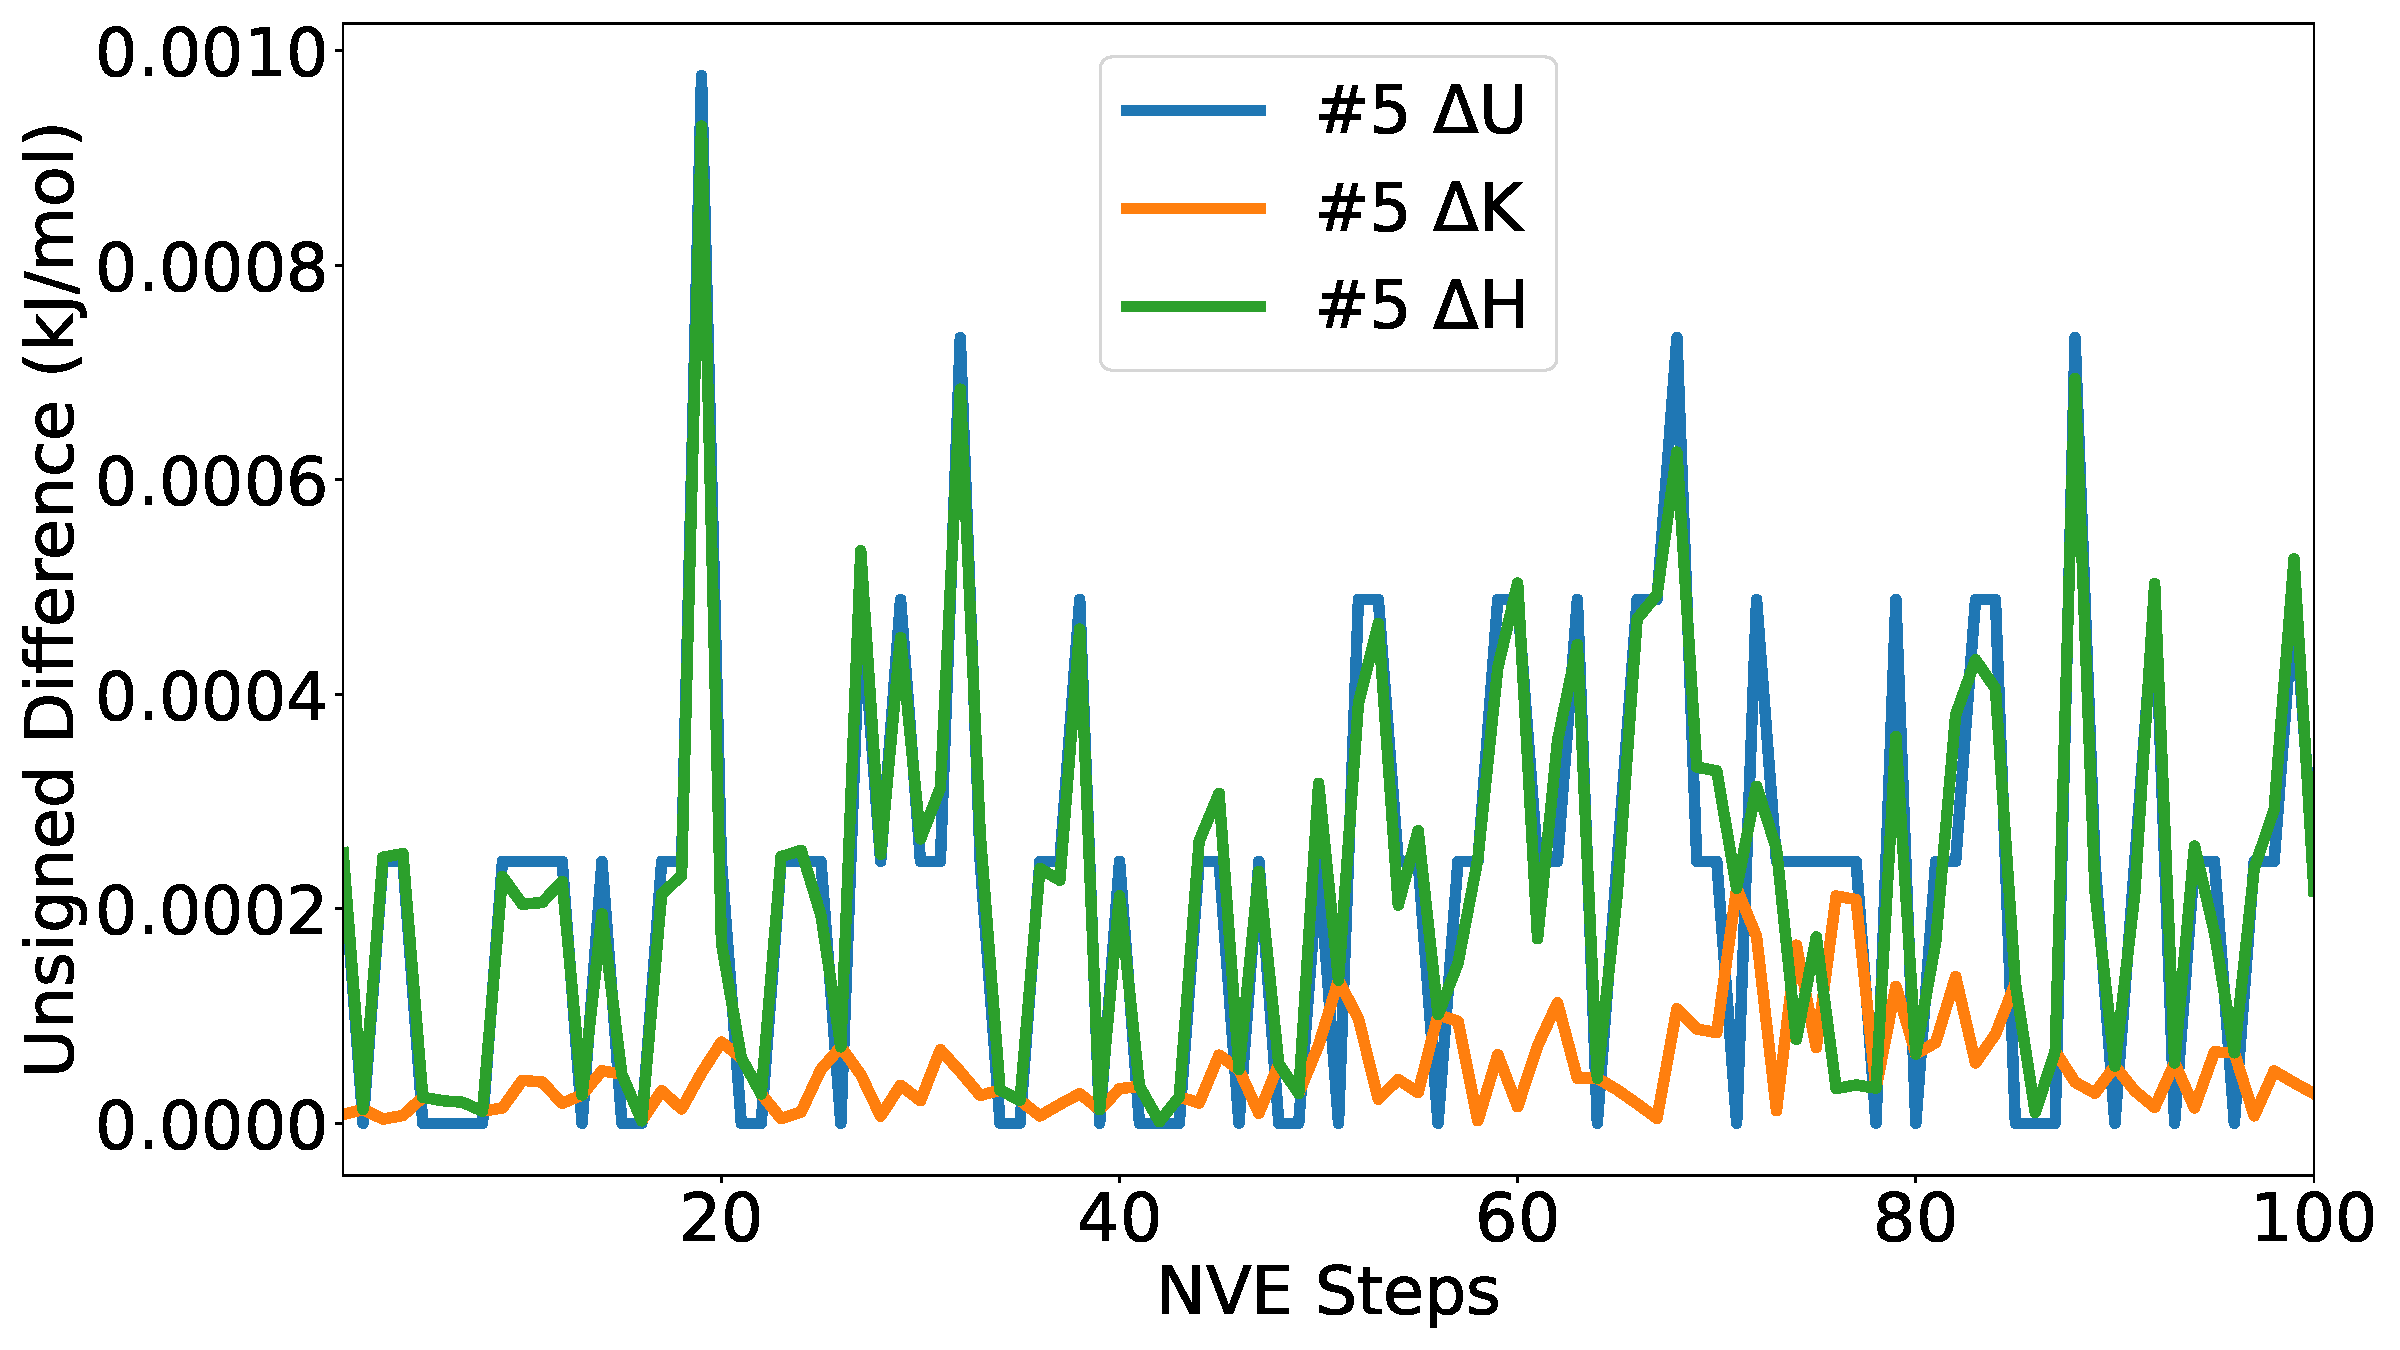
\includegraphics[width=\linewidth]{figs/div5.pdf}
\end{subfigure}
\begin{subfigure}{0.48\textwidth}
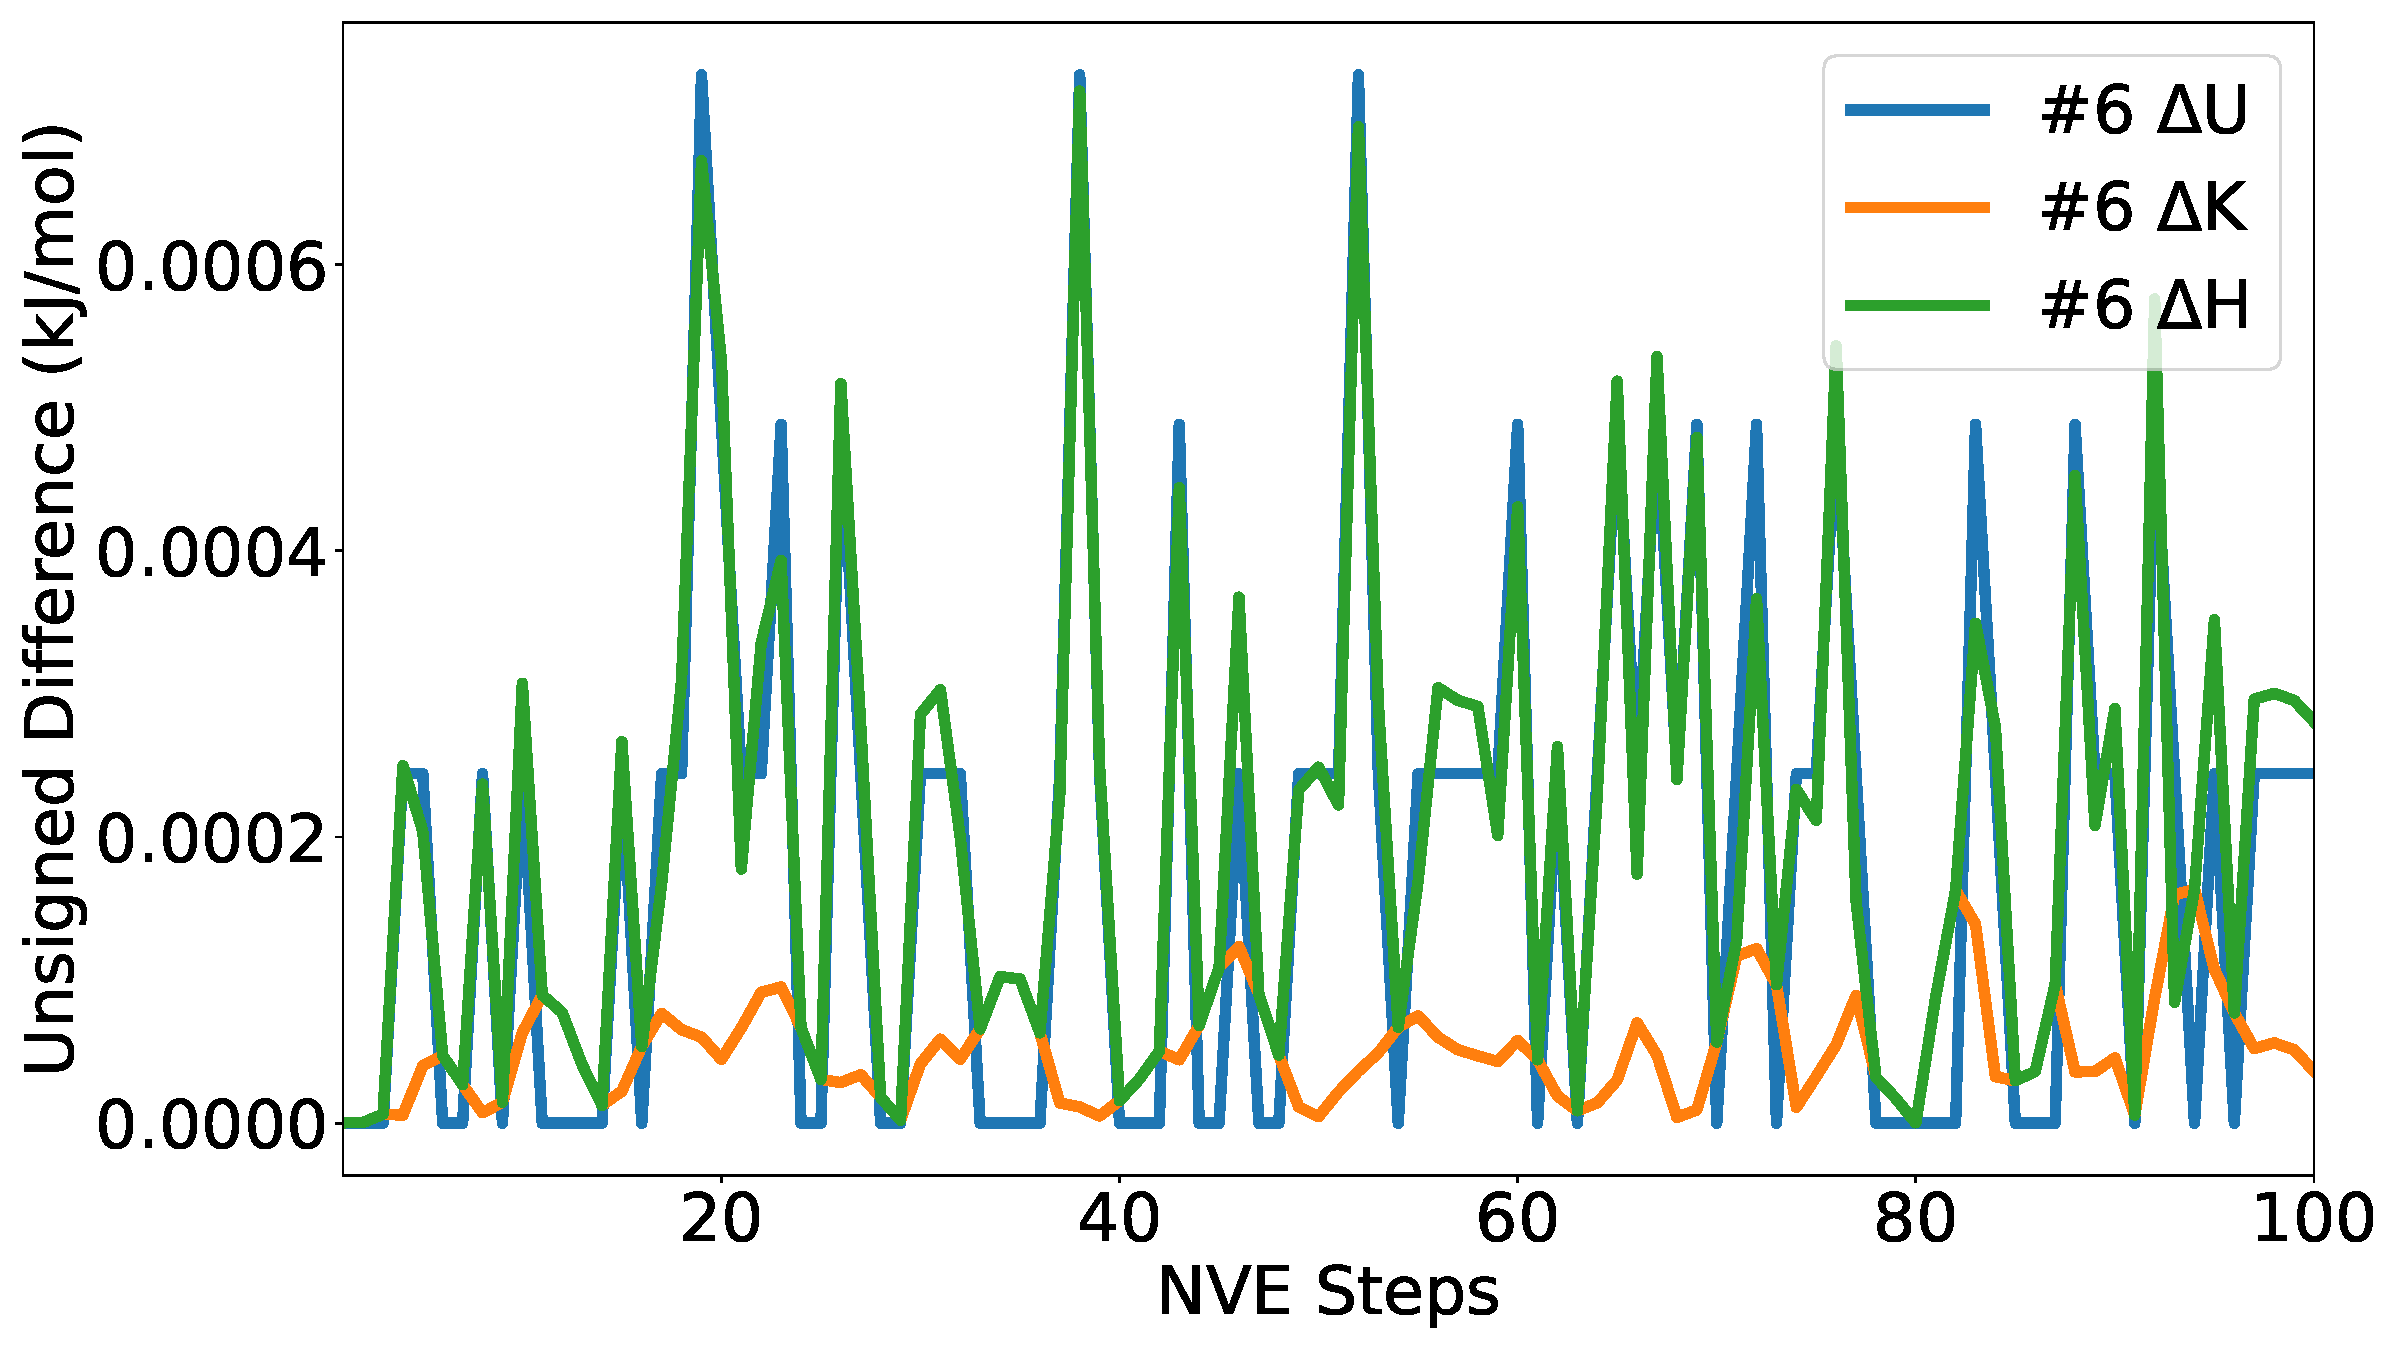
\includegraphics[width=\linewidth]{figs/div6.pdf}
\end{subfigure}
\\
\begin{subfigure}{0.48\textwidth}
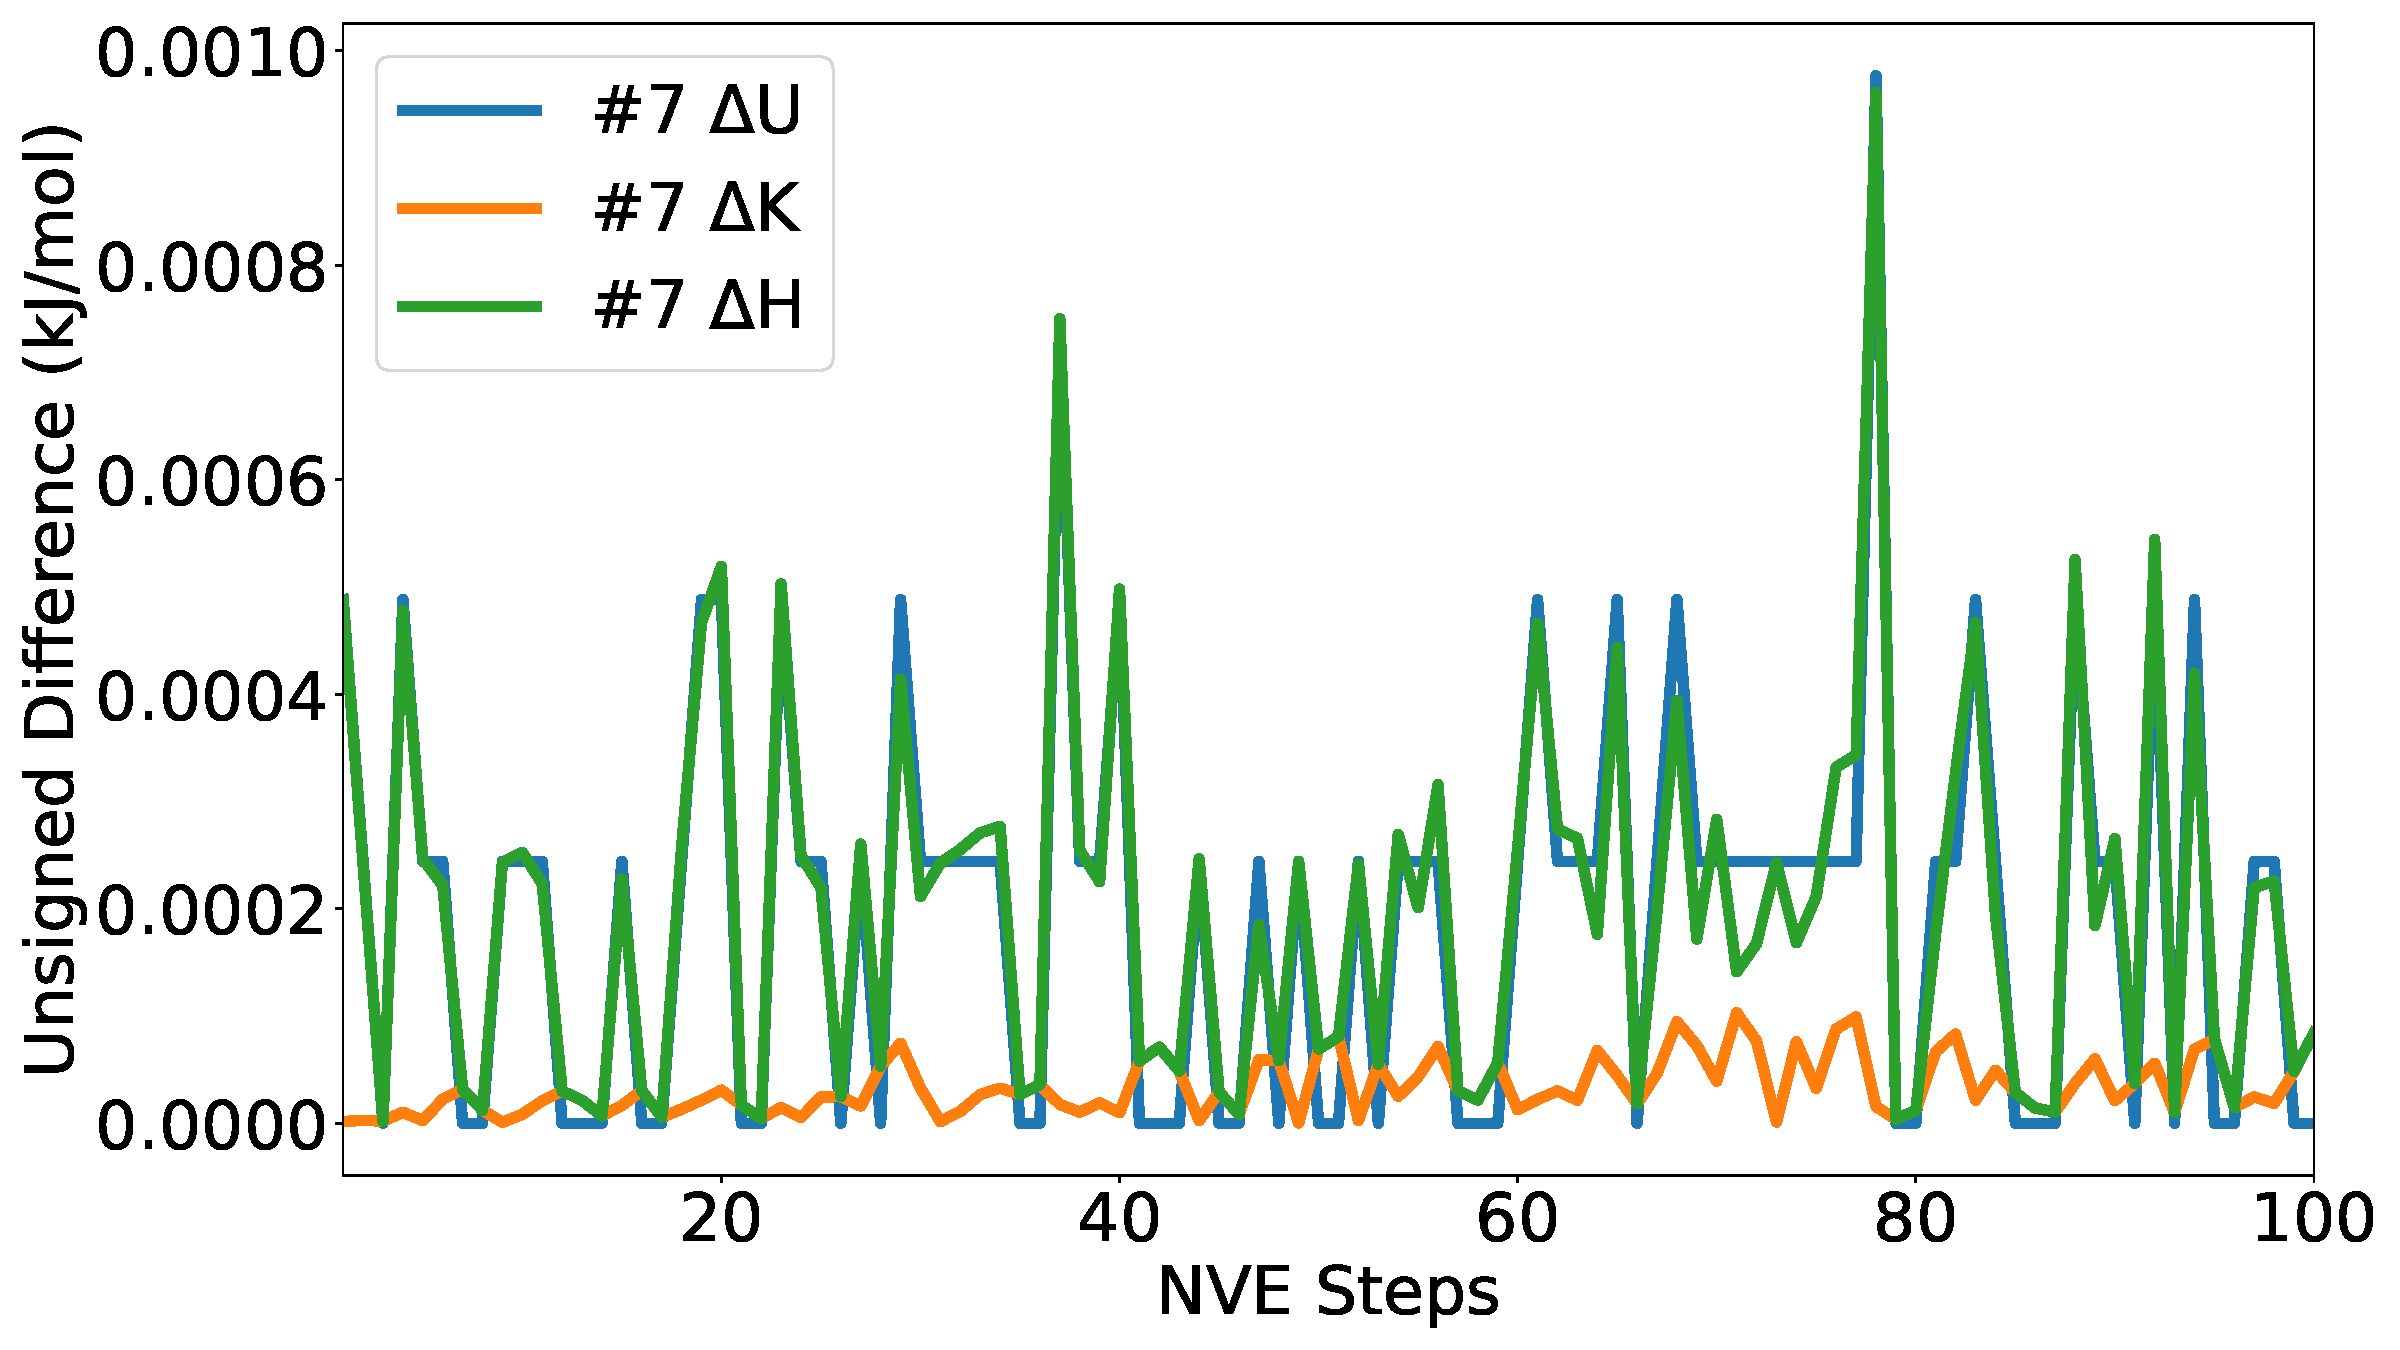
\includegraphics[width=\linewidth]{figs/div7.pdf}
\end{subfigure}
\begin{subfigure}{0.48\textwidth}
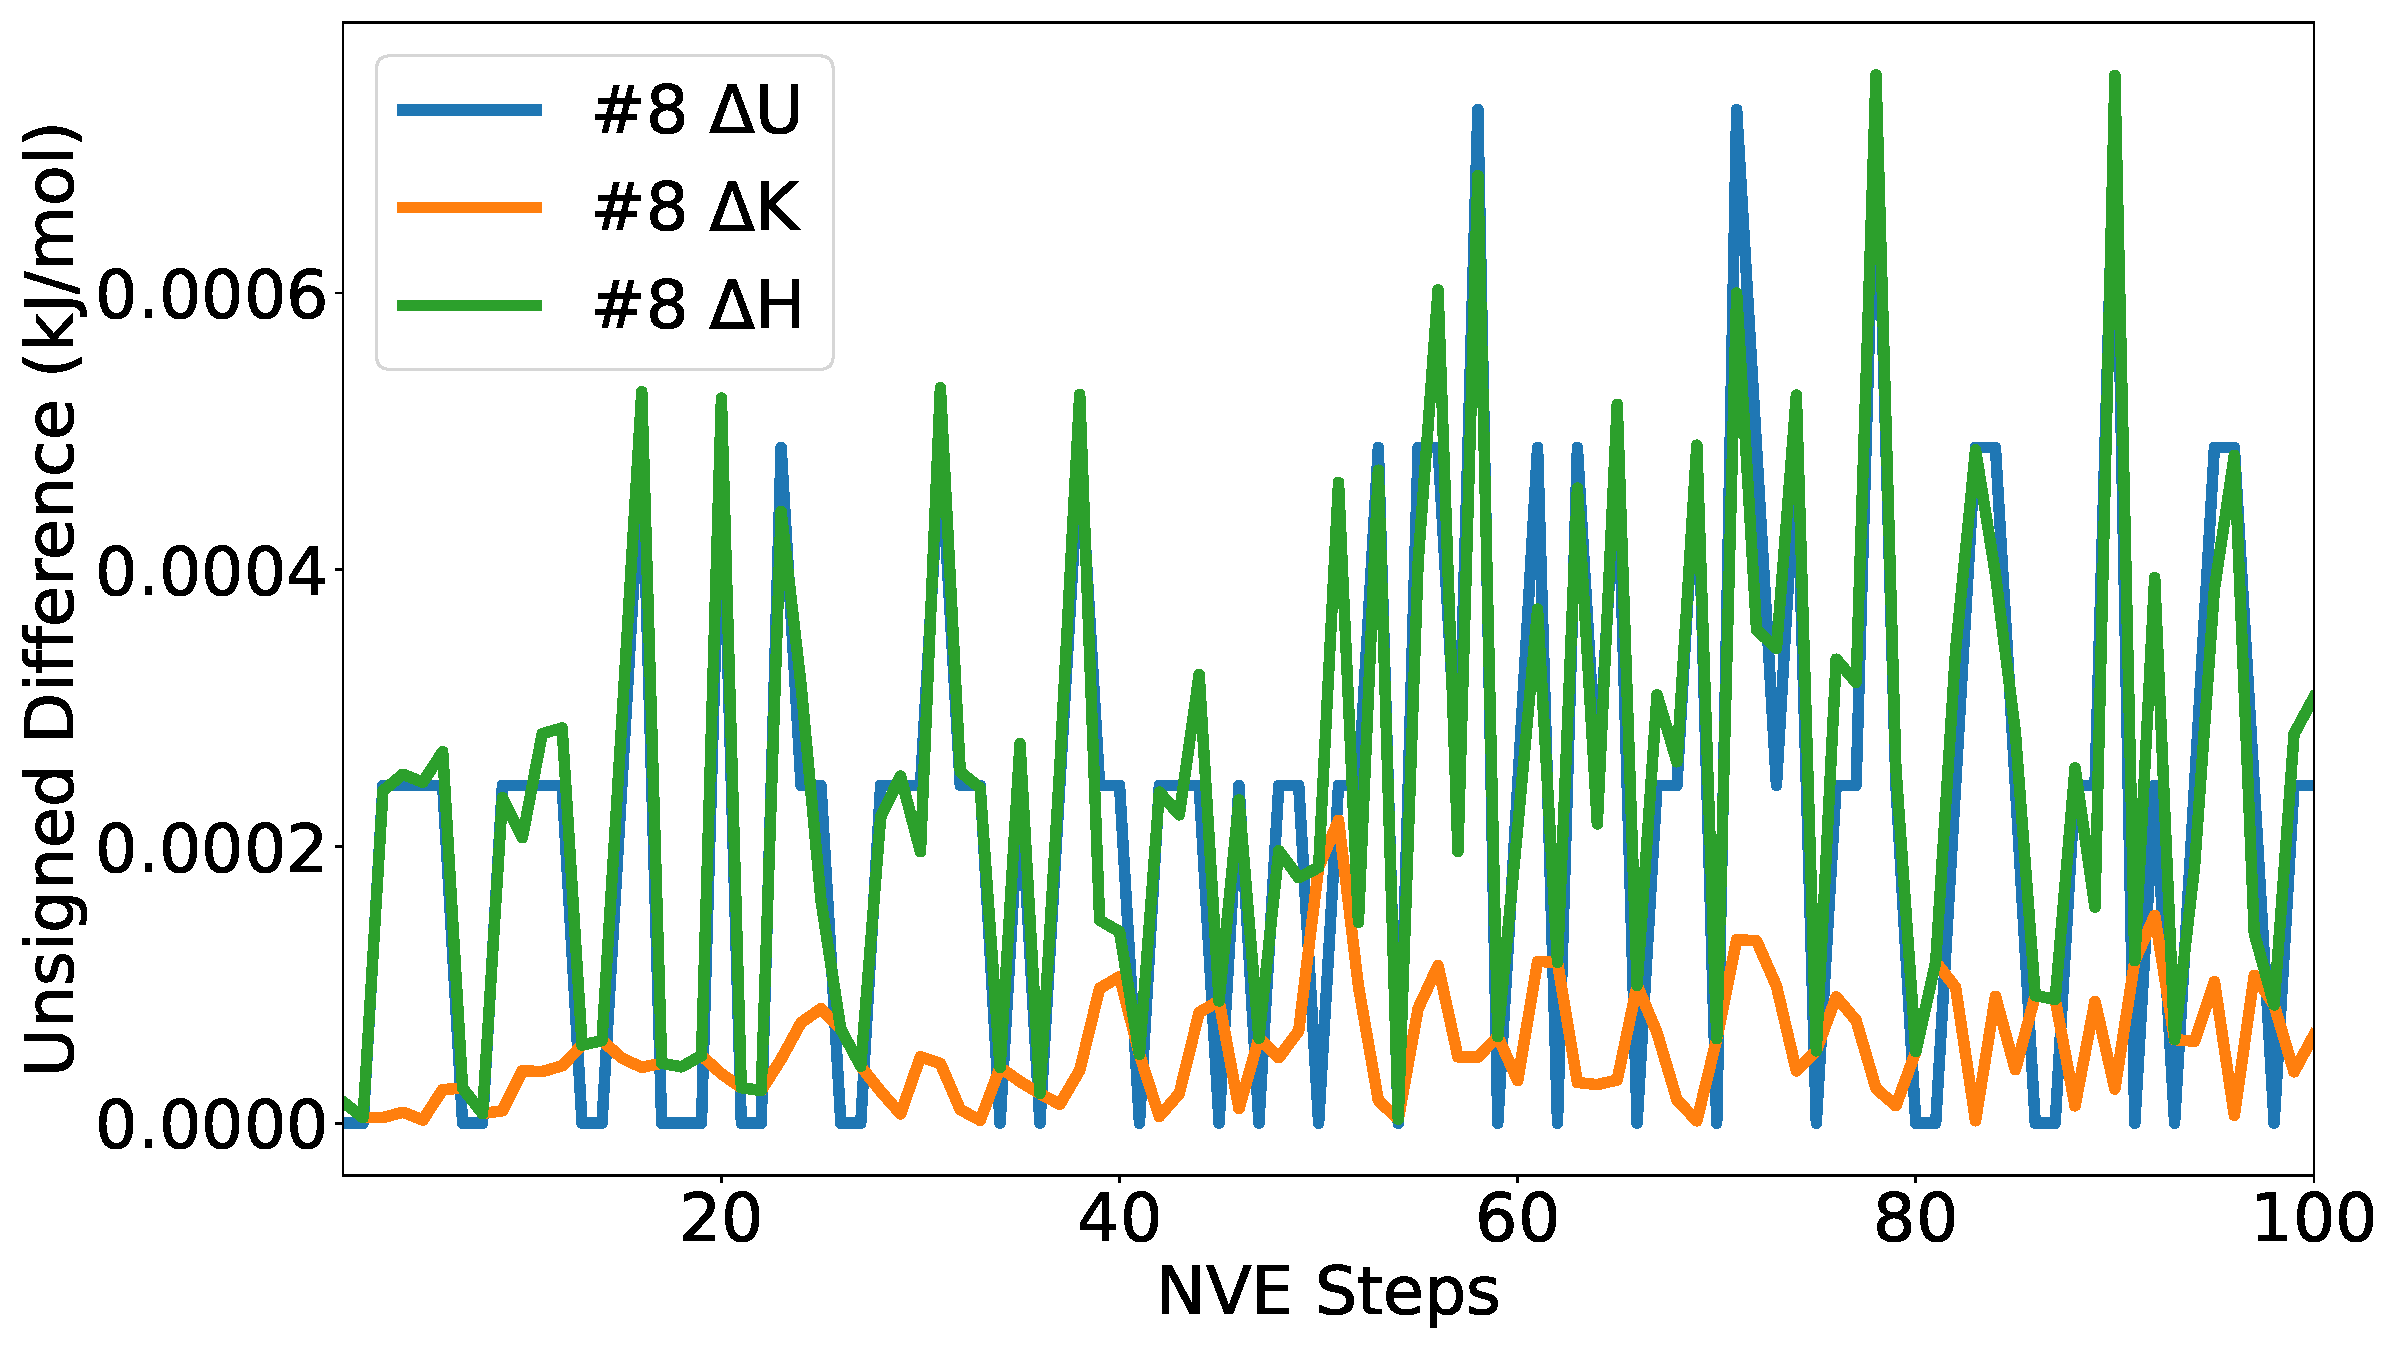
\includegraphics[width=\linewidth]{figs/div8.pdf}
\end{subfigure}
\caption{Comparison of energies across deployment strategies:
unsigned differences in potential energy ($U$), kinetic energy ($K$), and
Hamiltonian ($H$) relative to the baseline simulation over 100 time-steps.
The number in each subfigure indicates the deployment method
as defined in Table~\ref{tb:deploy8}.}\label{fig:convergence}
\end{figure*}

\else\fi

\textbf{Errors in Forces}
Using the baseline trajectory, we recalculated the potential energies and forces.
Figure~\ref{fig:reruns} illustrates the unsigned error in potential energies
and root mean square deviation (RMSD) of the 27 force components
relative to the baseline values.
These results corroborate that the differences are minimal,
reaching the inherent precision limit of fp32 arithmetic.

\ifdefined\InlineFloatEnv
\begin{figure*}[htbp]
\begin{subfigure}{0.48\textwidth}
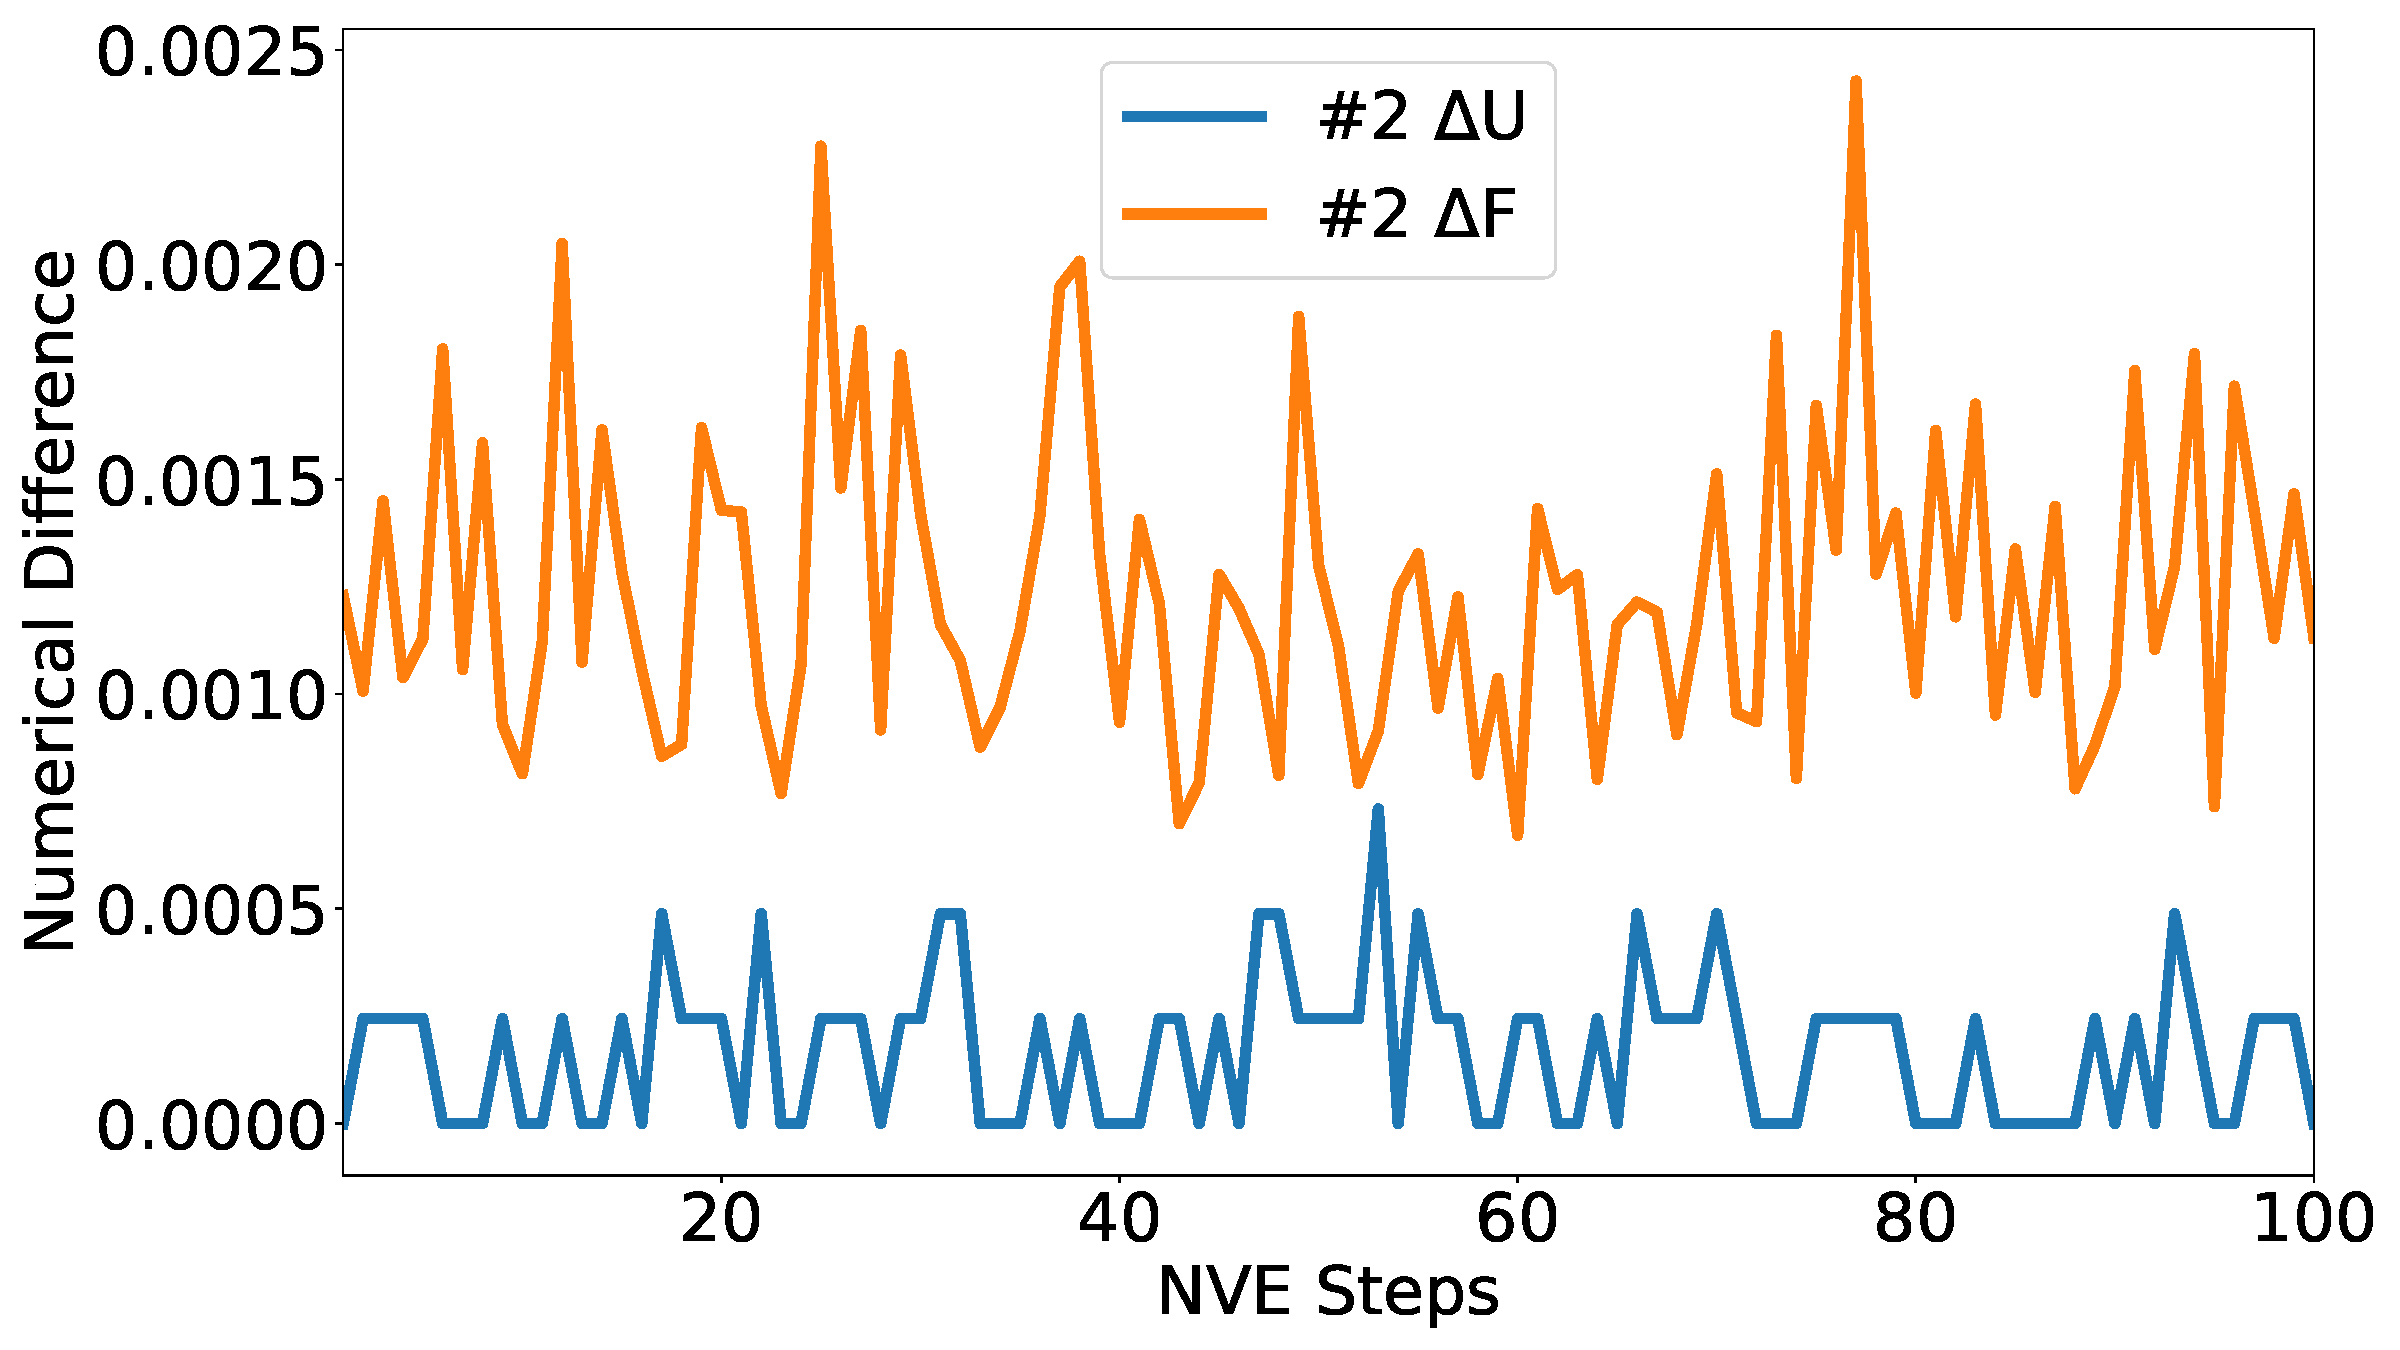
\includegraphics[width=\linewidth]{figs/rerun2.pdf}
\end{subfigure}
\\
\begin{subfigure}{0.48\textwidth}
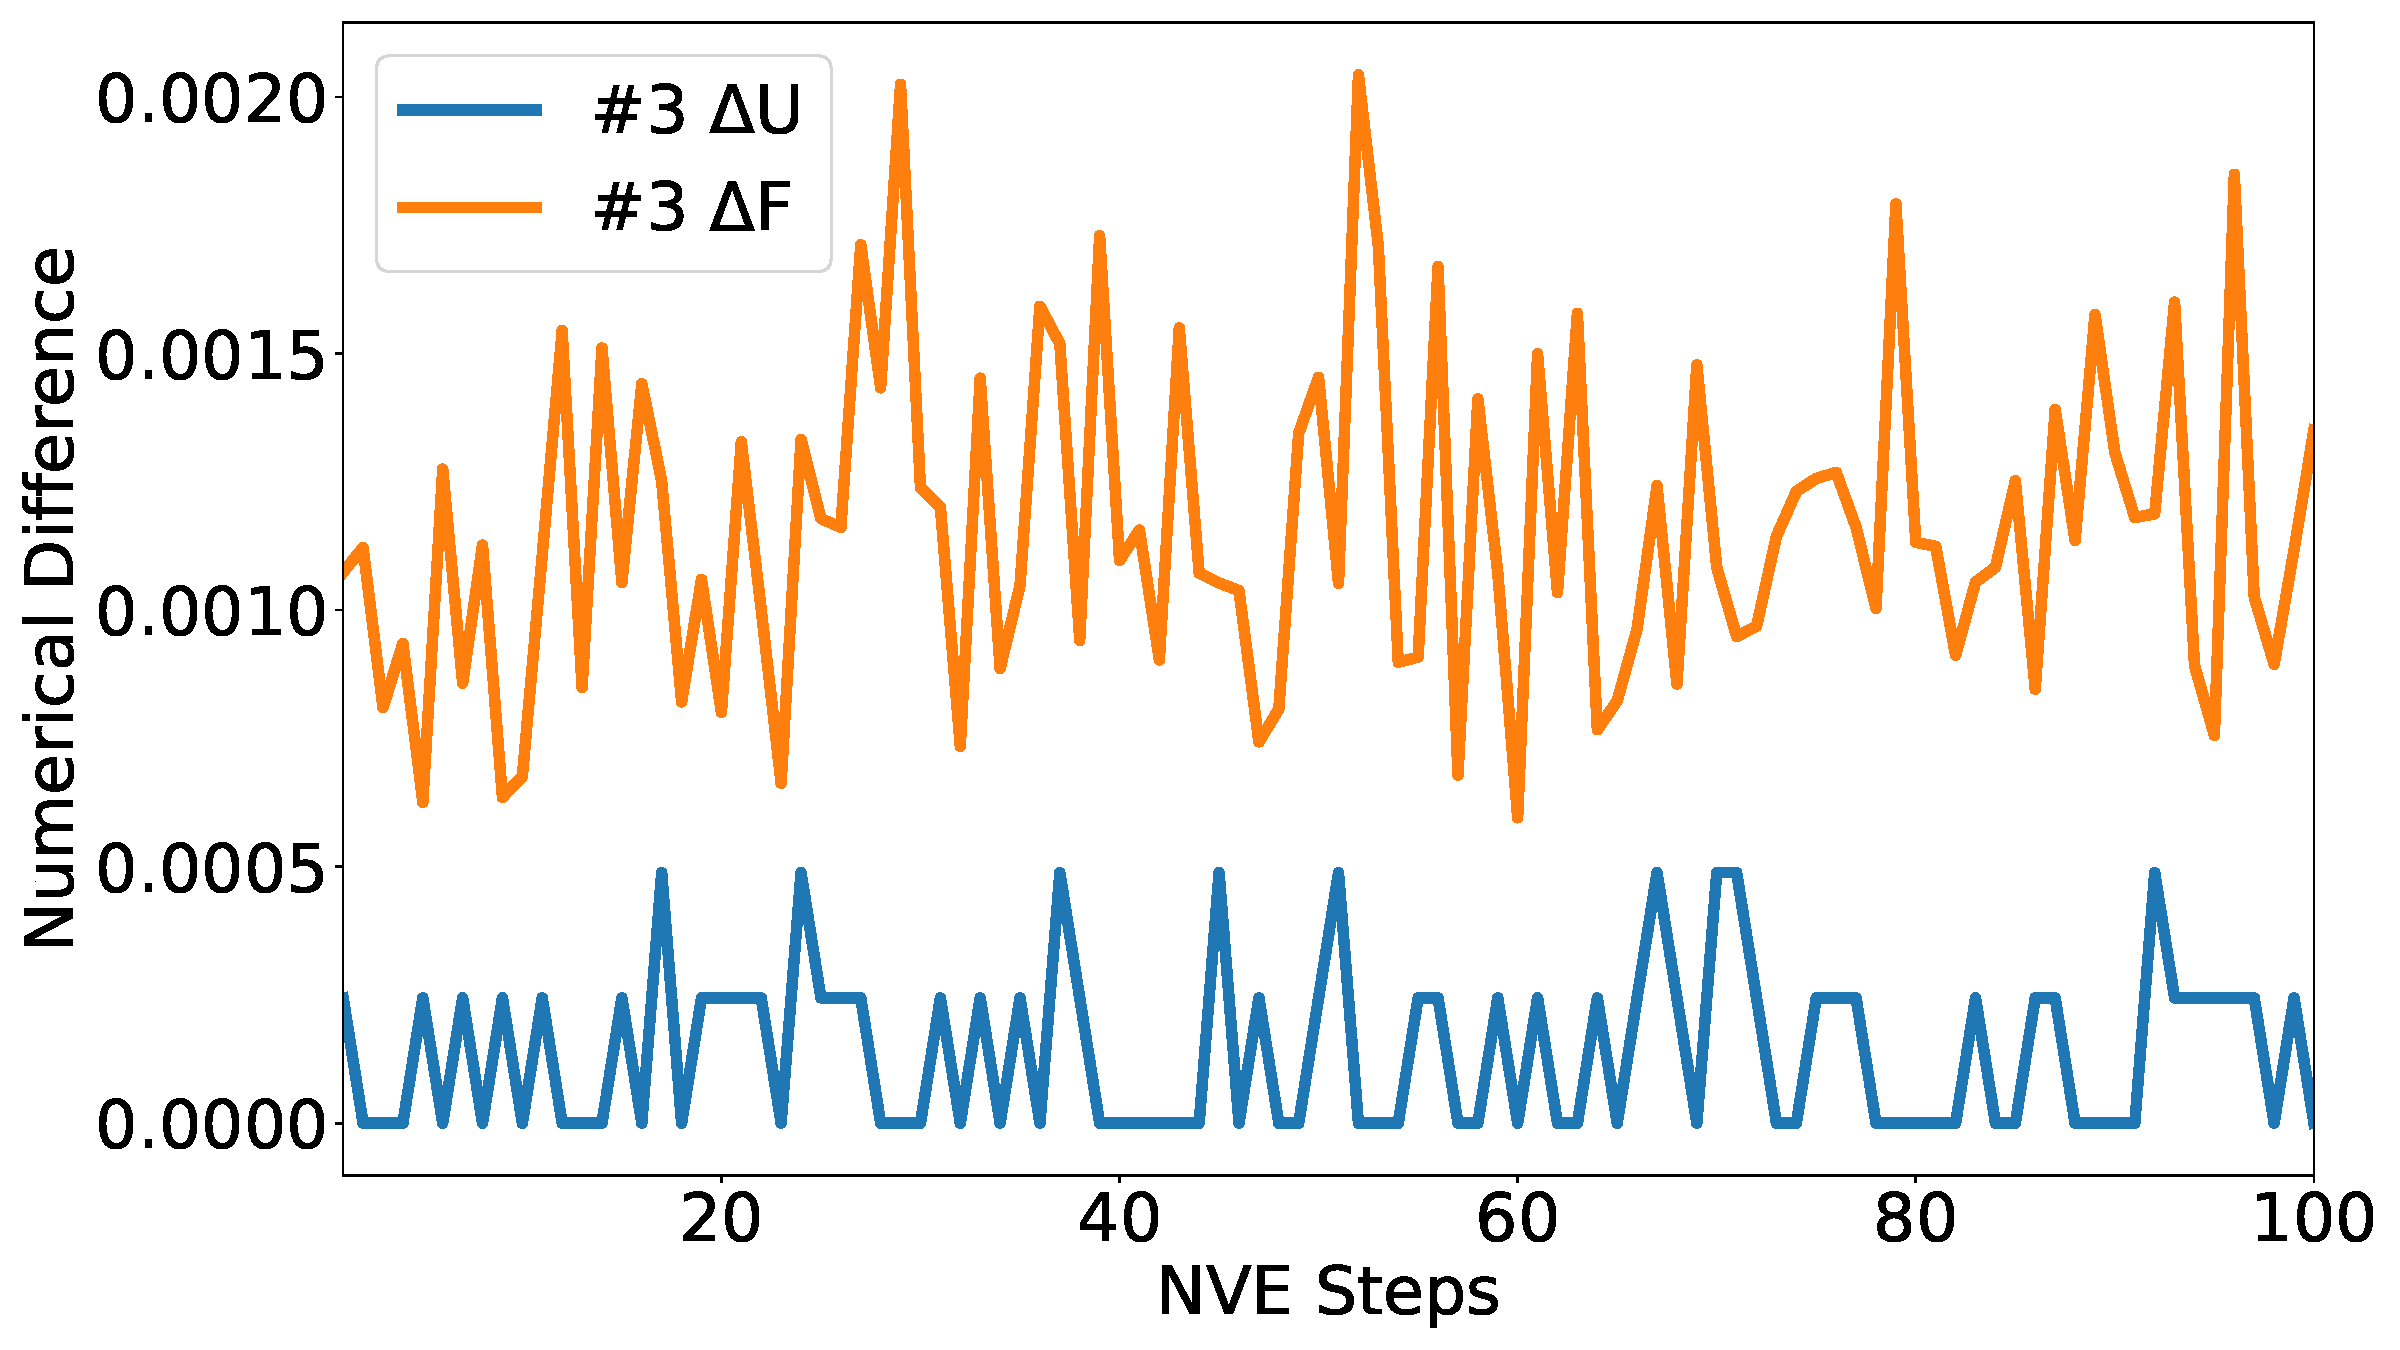
\includegraphics[width=\linewidth]{figs/rerun3.pdf}
\end{subfigure}
\begin{subfigure}{0.48\textwidth}
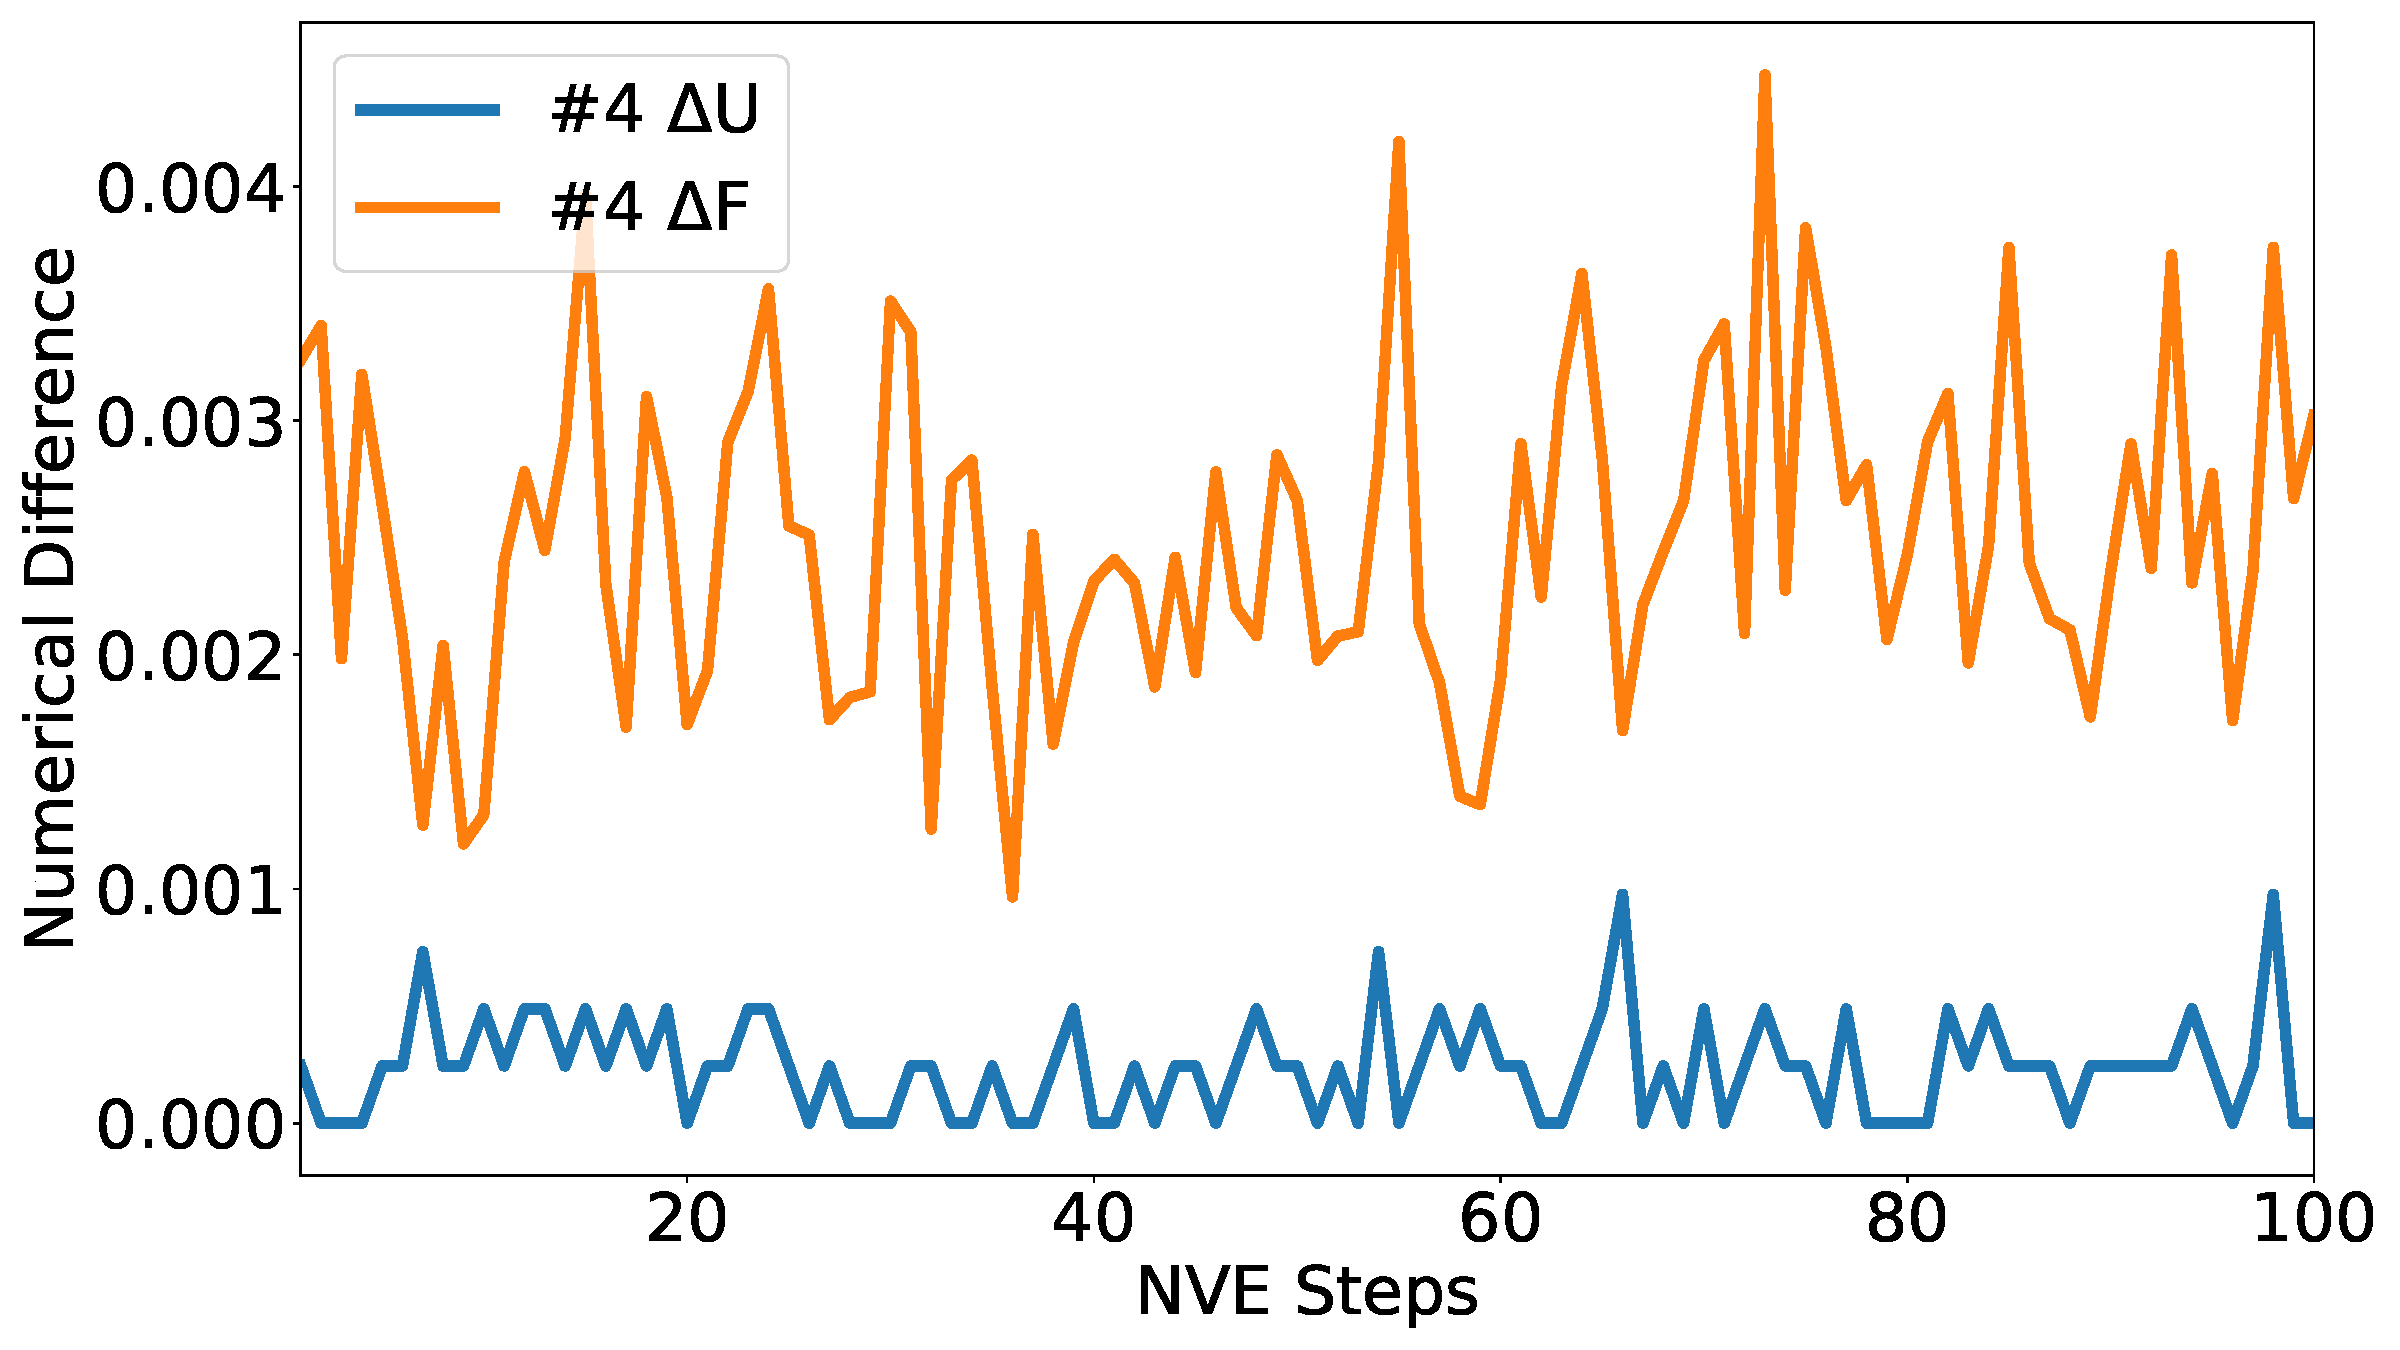
\includegraphics[width=\linewidth]{figs/rerun4.pdf}
\end{subfigure}
\\
\begin{subfigure}{0.48\textwidth}
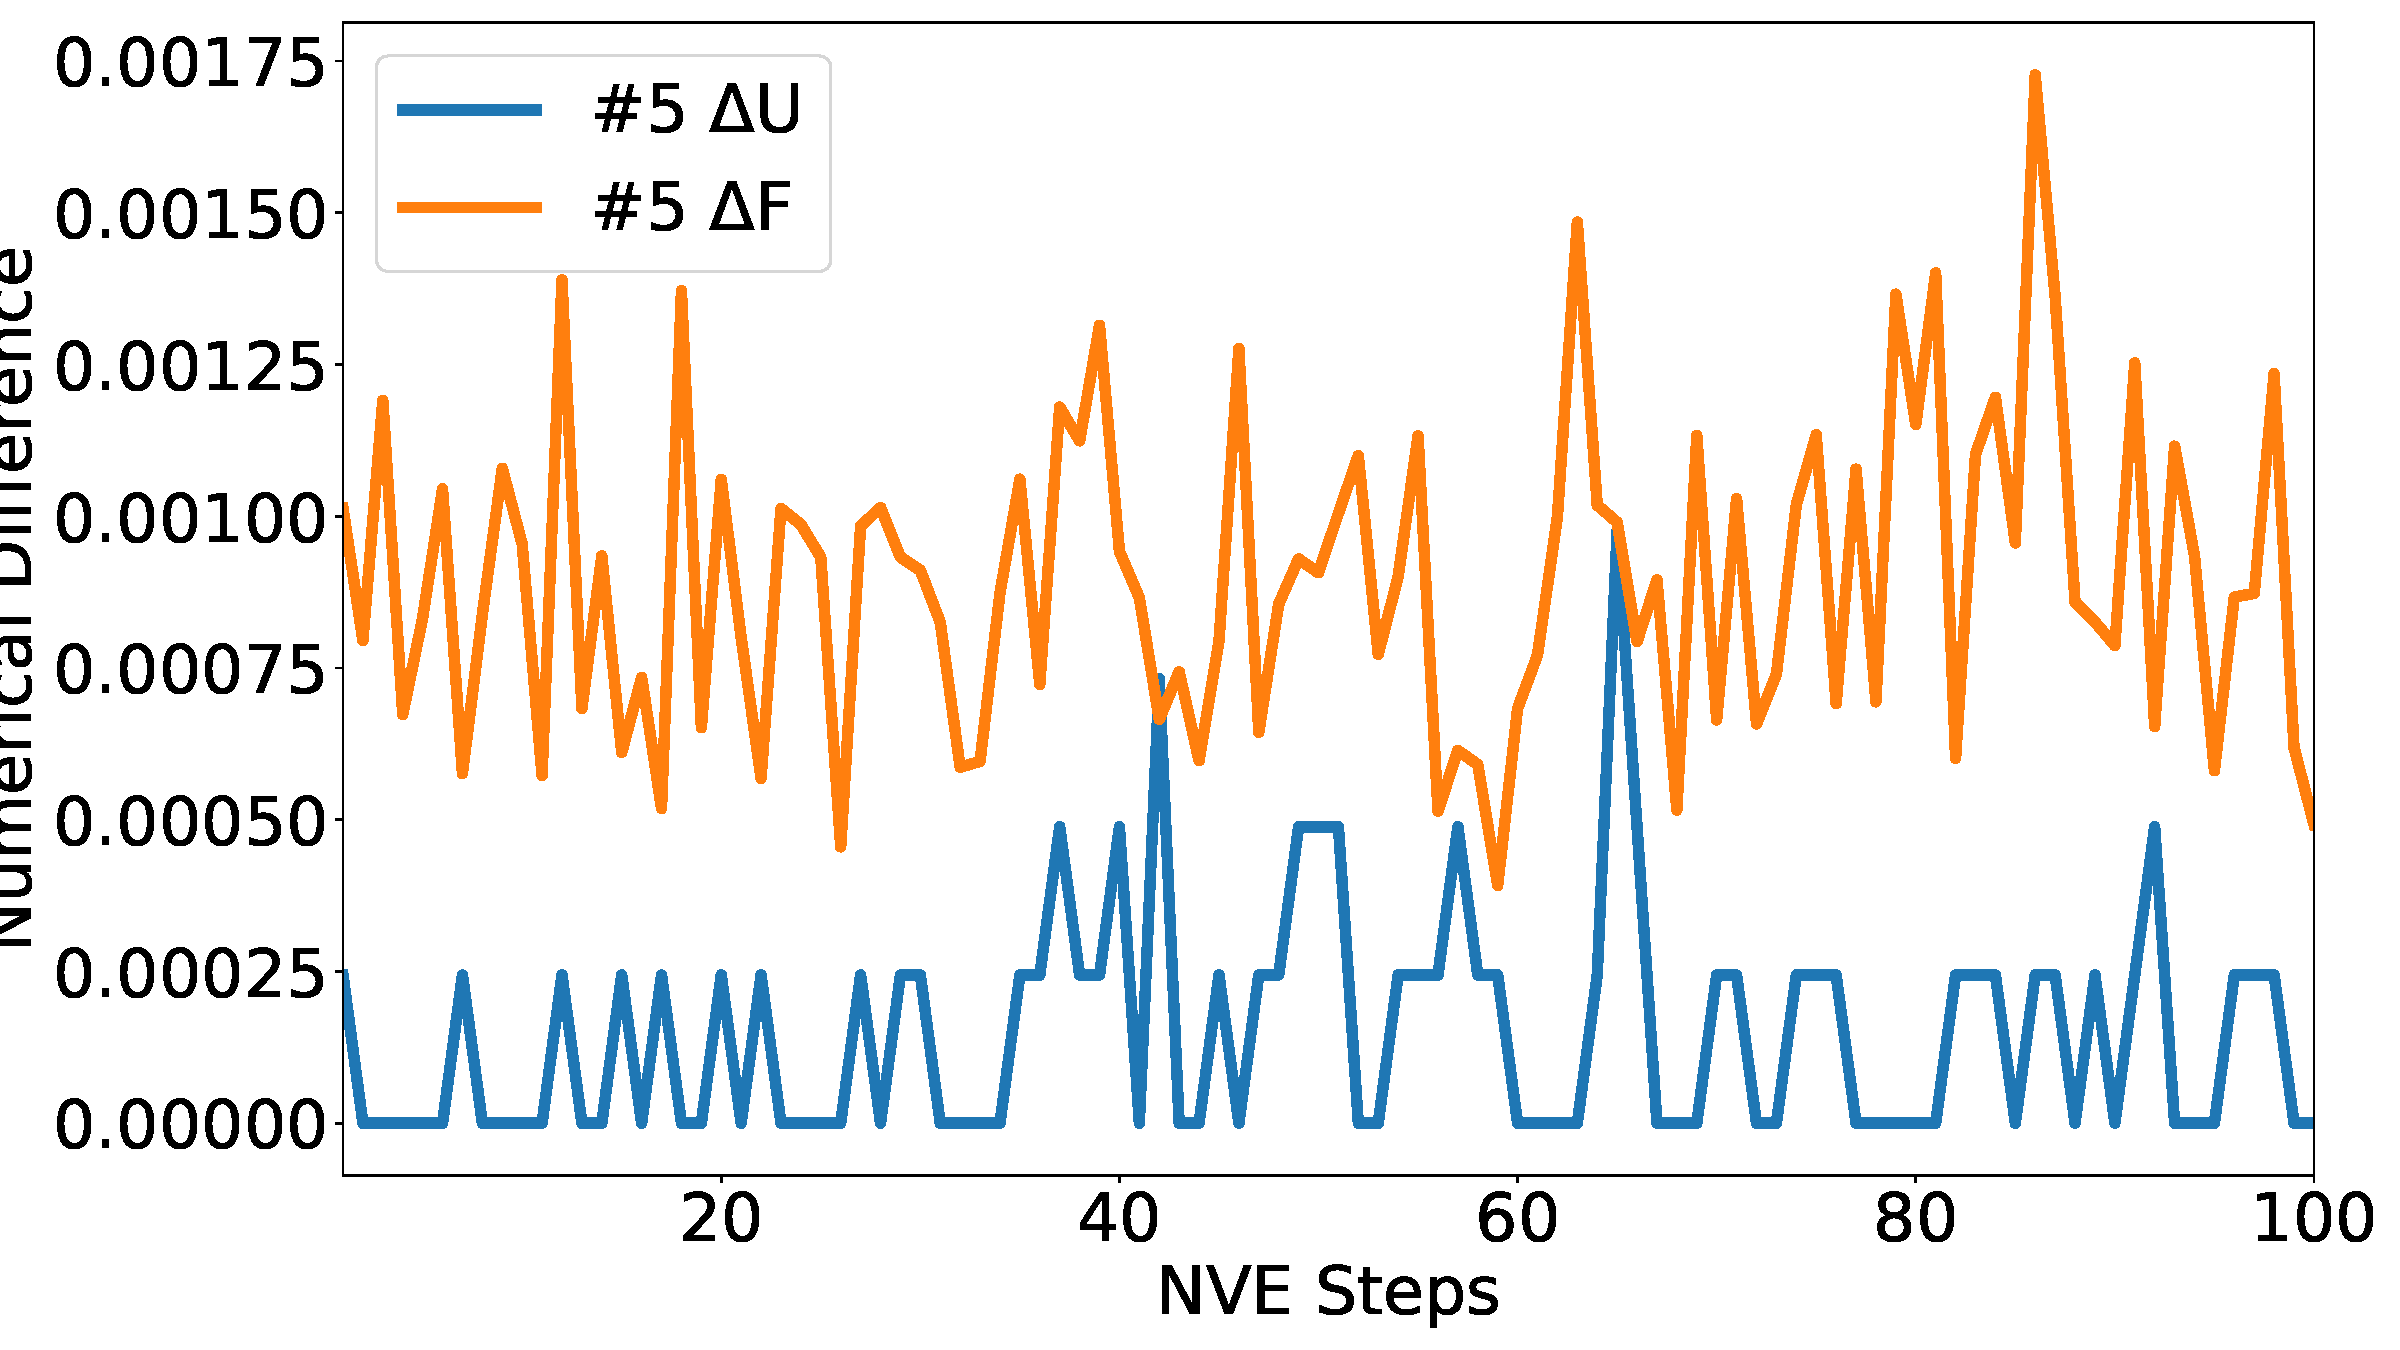
\includegraphics[width=\linewidth]{figs/rerun5.pdf}
\end{subfigure}
\begin{subfigure}{0.48\textwidth}
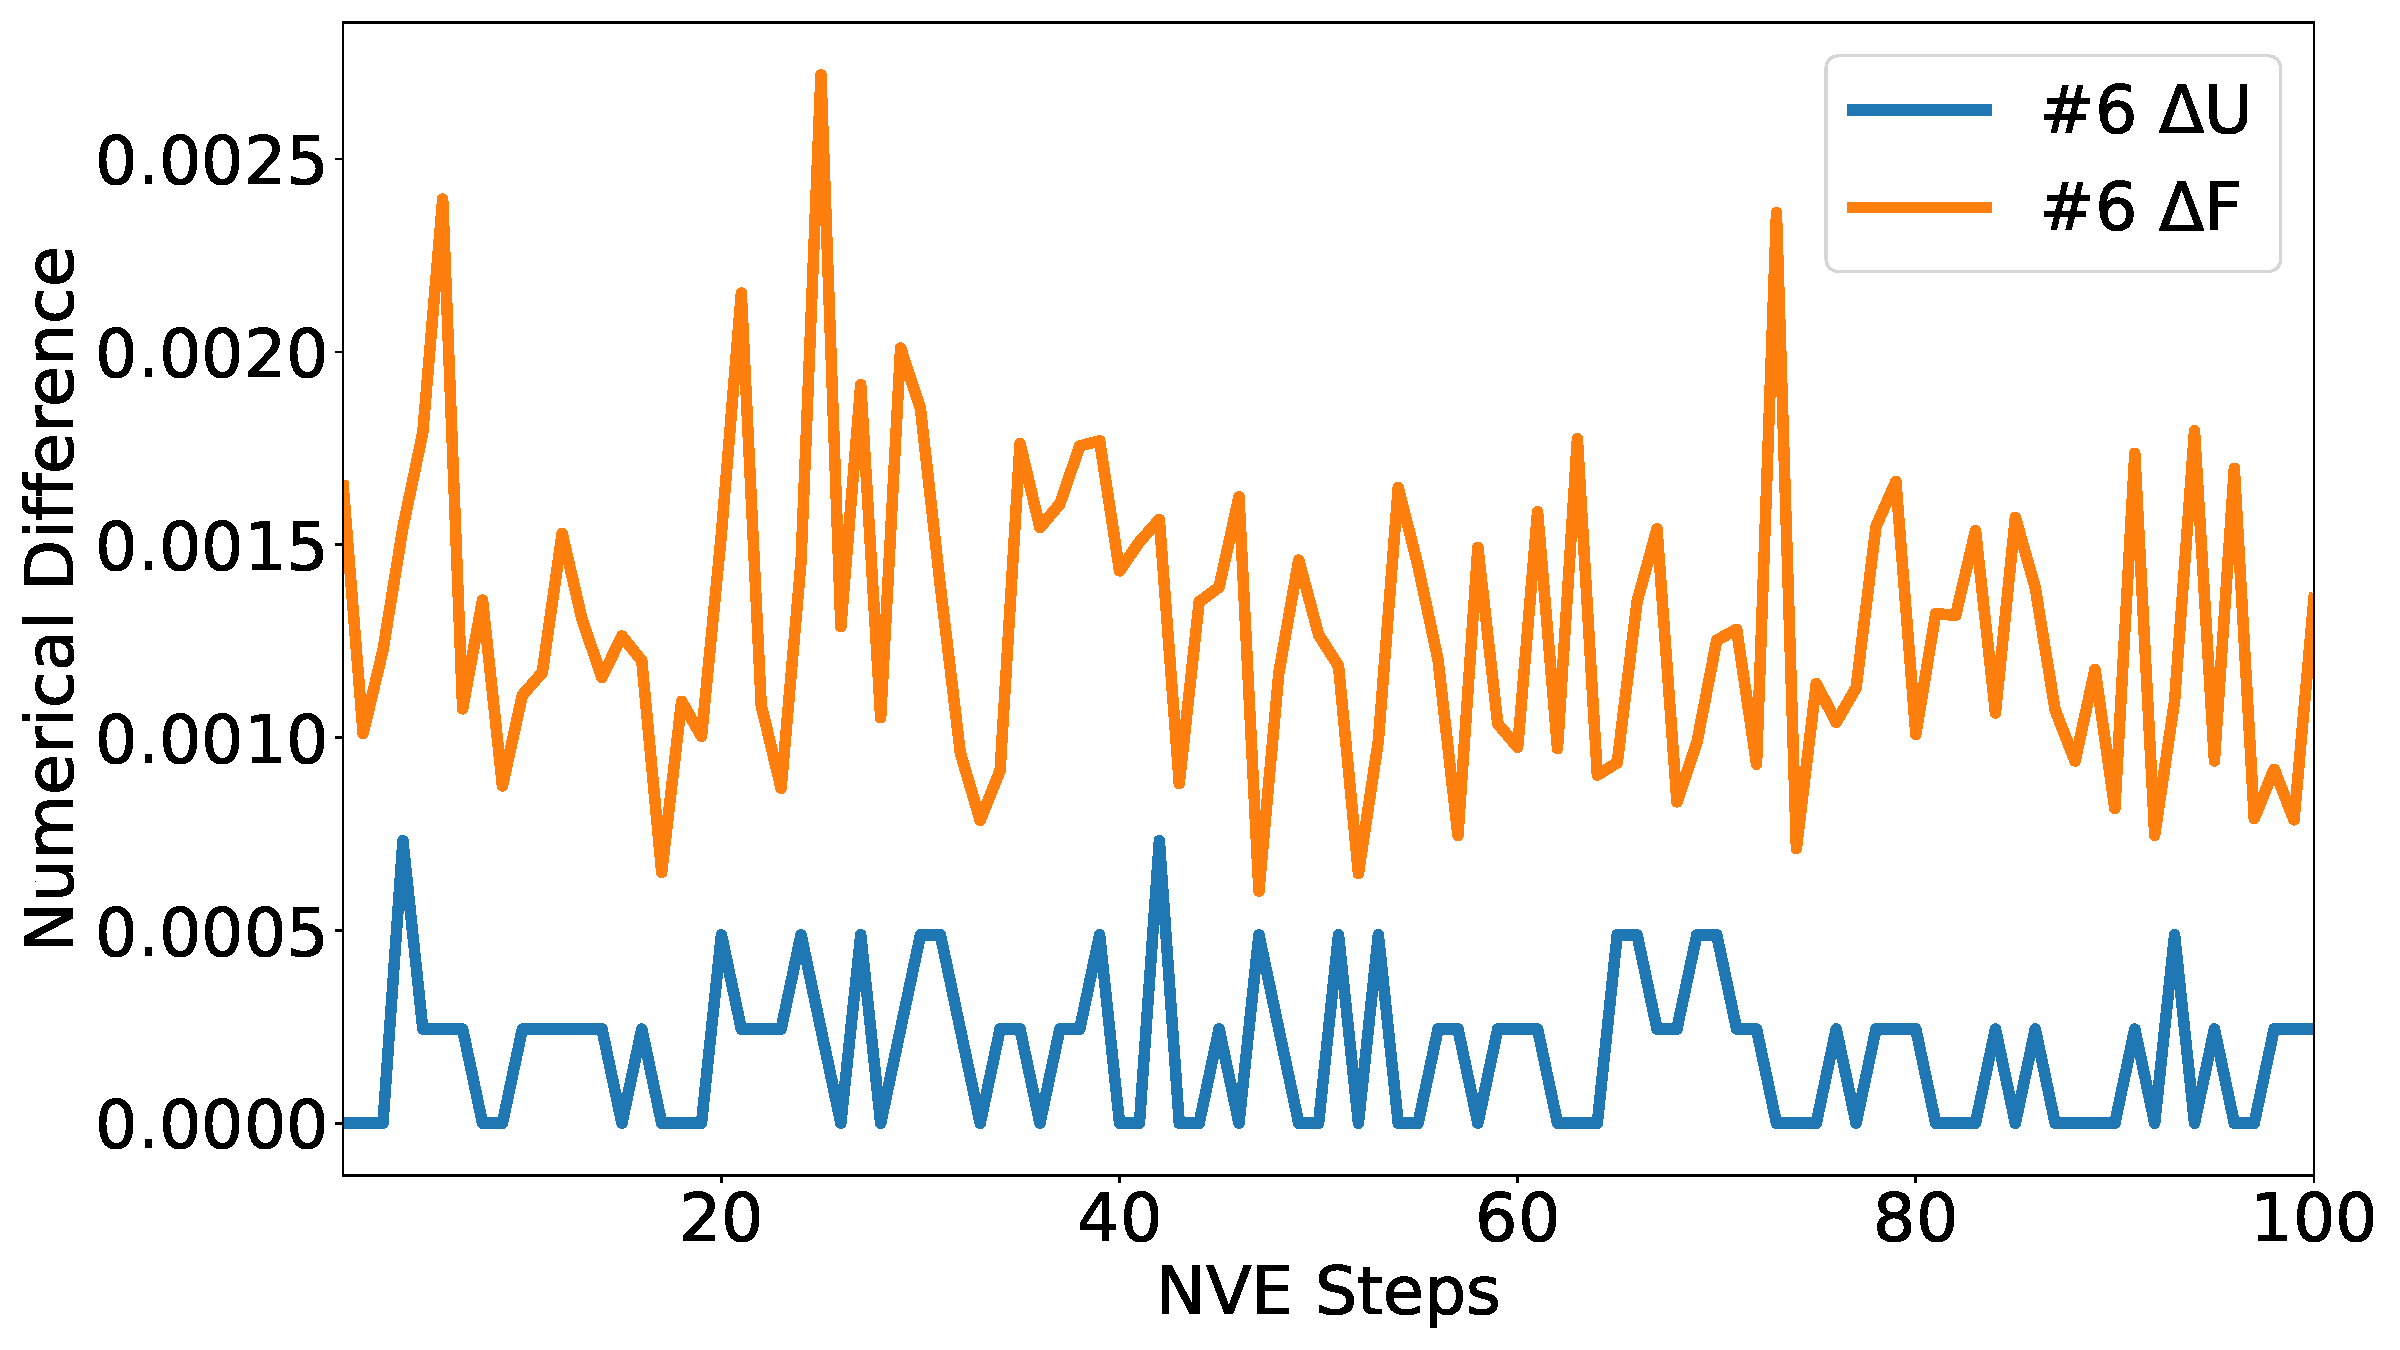
\includegraphics[width=\linewidth]{figs/rerun6.pdf}
\end{subfigure}
\\
\begin{subfigure}{0.48\textwidth}
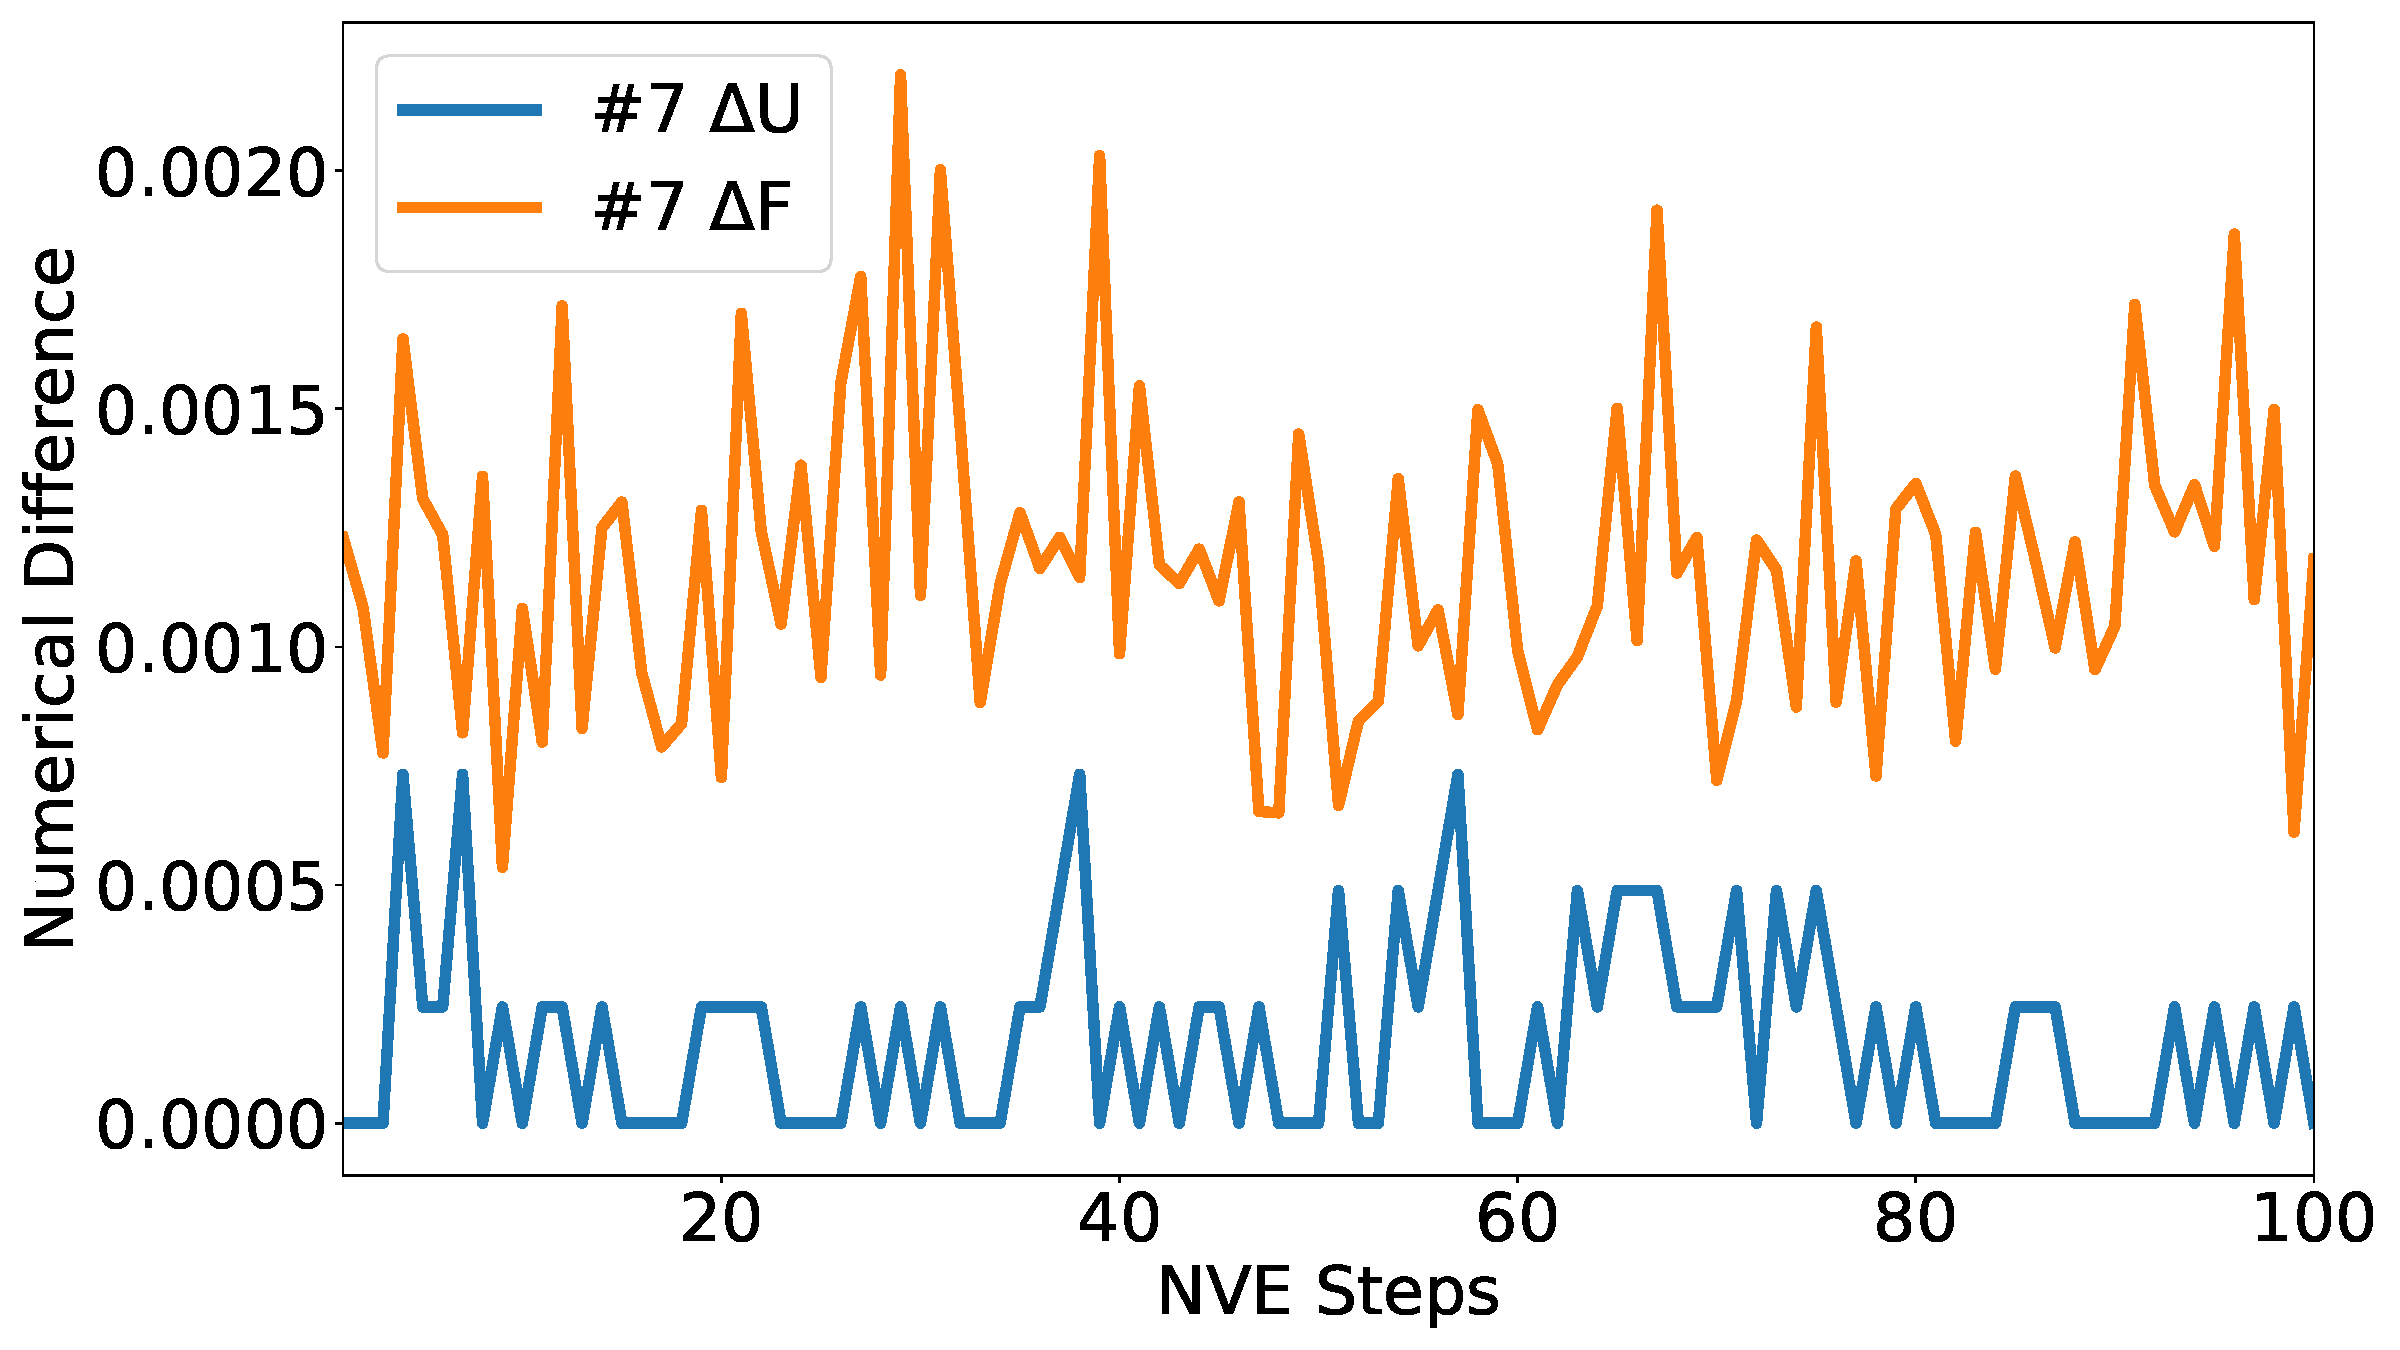
\includegraphics[width=\linewidth]{figs/rerun7.pdf}
\end{subfigure}
\begin{subfigure}{0.48\textwidth}
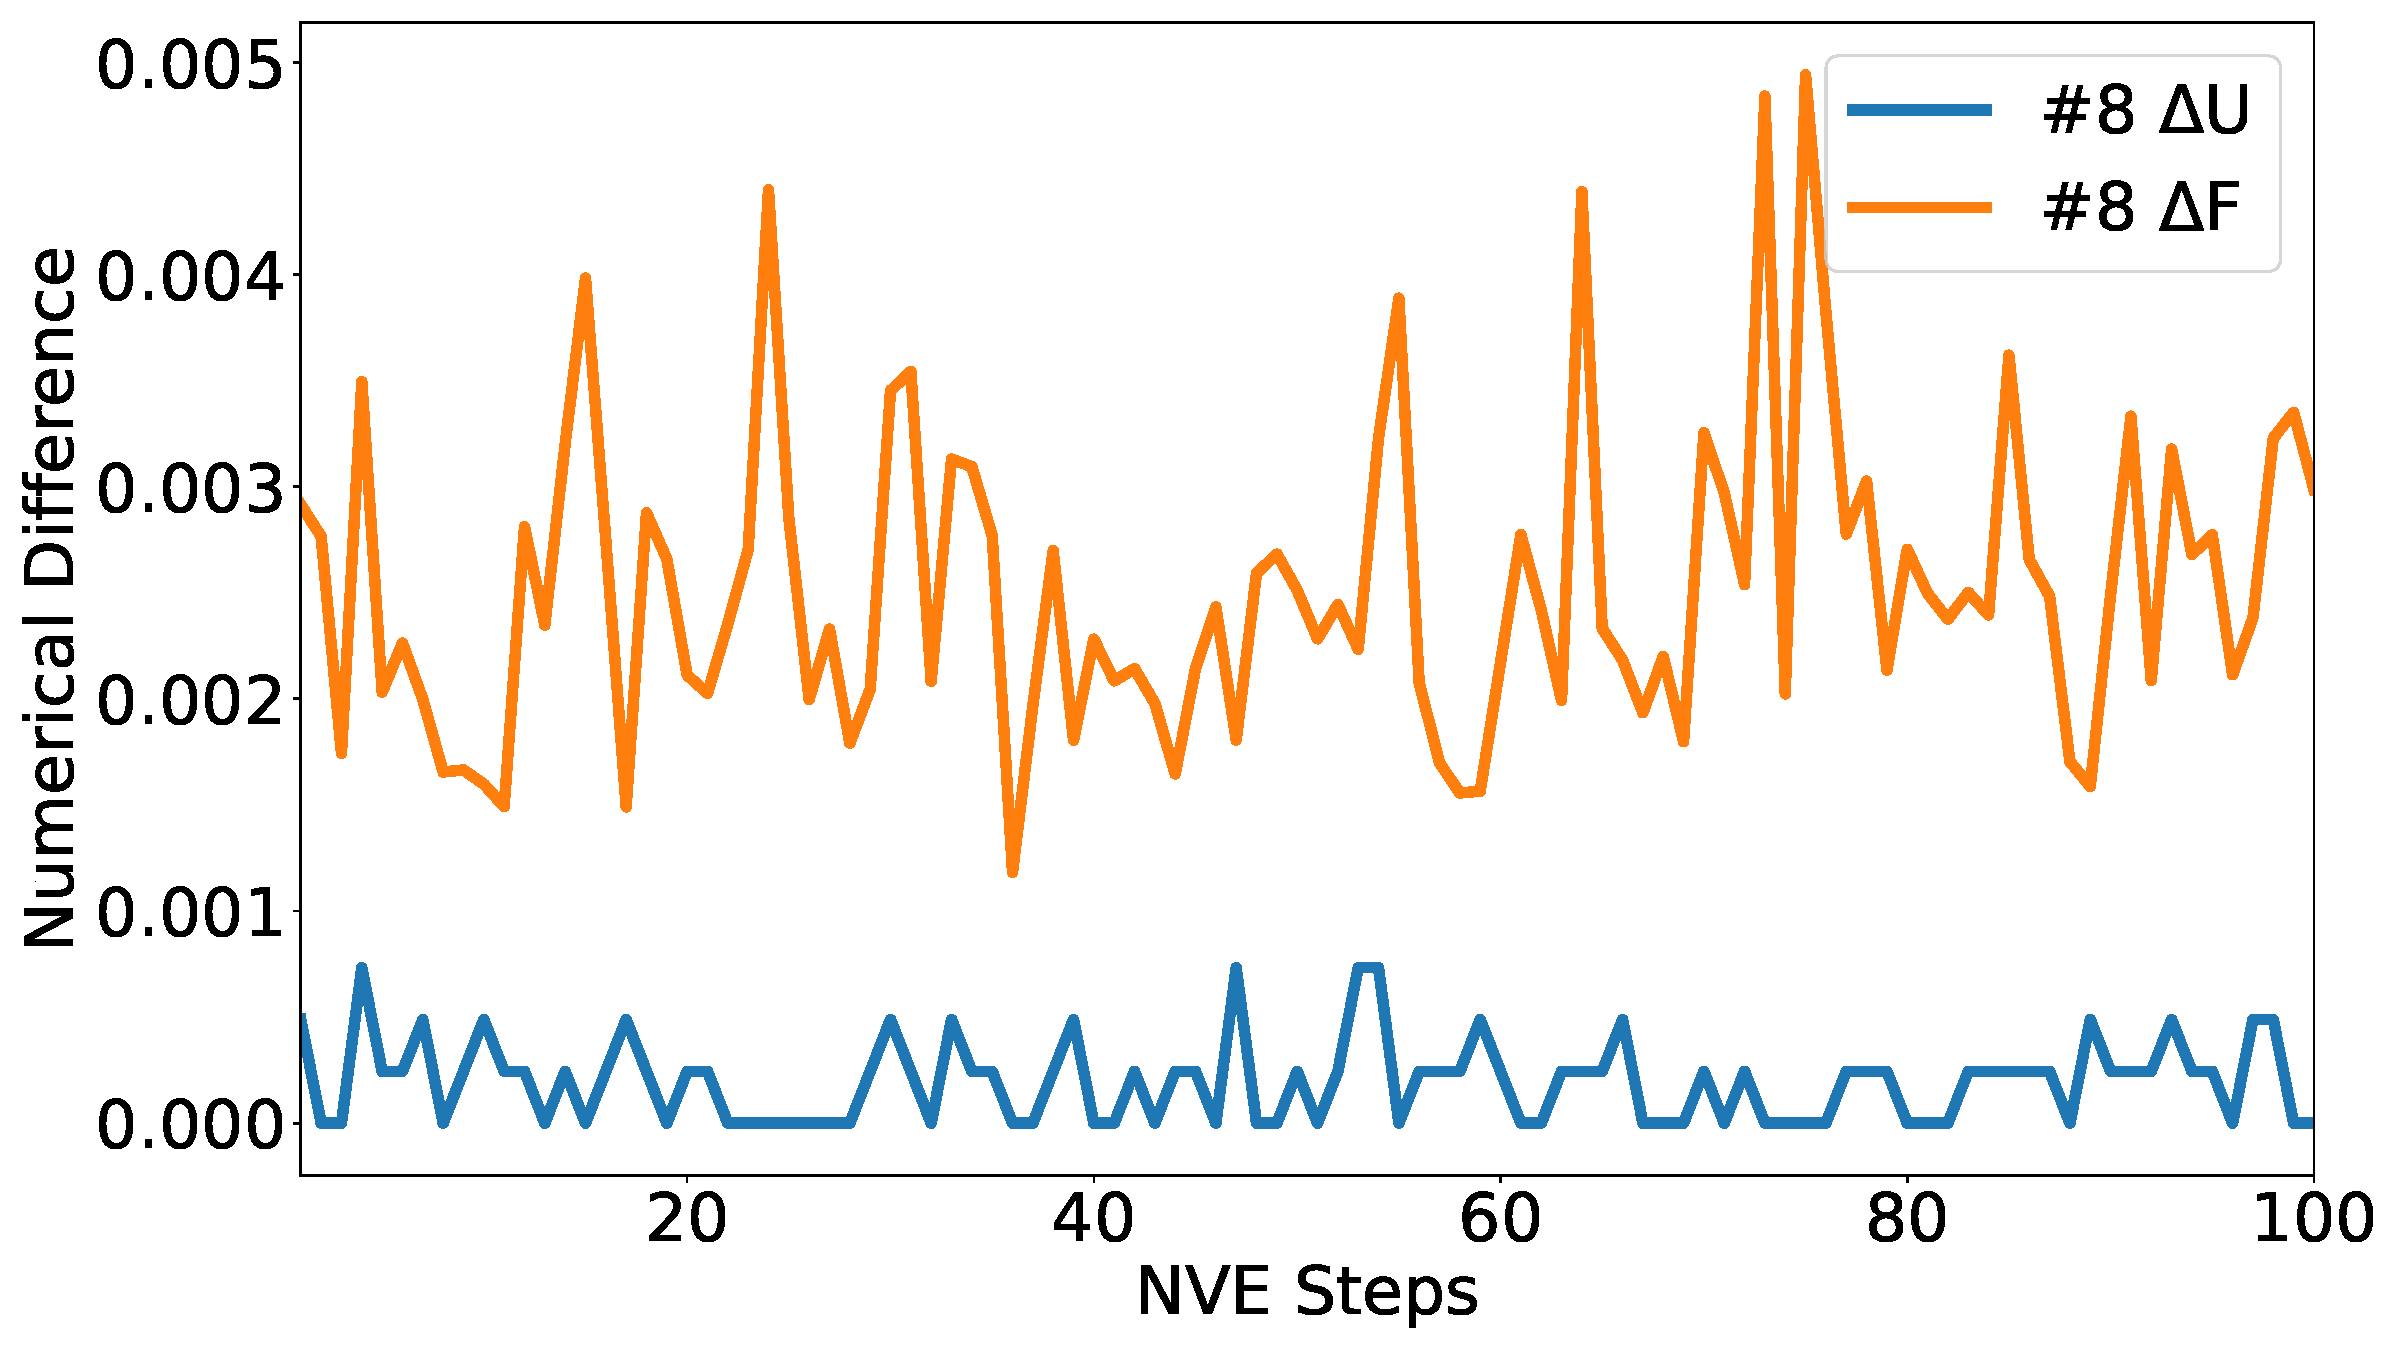
\includegraphics[width=\linewidth]{figs/rerun8.pdf}
\end{subfigure}
\caption{The unsigned differences in potential energies
and root mean square deviation of forces (in kJ/mol and nm)
compared to the baseline,
obtained by recalculating an identical PDB trajectory
across deployment methods.
The number in each subfigure denotes the deployment method
as defined in Table~\ref{tb:deploy8}.}
\label{fig:reruns}
\end{figure*}

\else\fi

The comparative performance of the eight strategies is summarized
in Table~\ref{tb:speed8}.
Performance benchmarks were conducted
using a Langevin integrator with a friction
of $0.1$~ps\textsuperscript{-1} over 1000 time-steps,
generating 10 trajectory frames.
For small-scale test cases such as a single ethanol molecule,
where kernel launch overhead dominates computational cost,
CUDA Graph significantly enhanced performance.
Comparisons between implementations 1 and 3, as well as 5 and 7,
demonstrate that direct inference via C++ APIs achieves superior performance
with reduced launch overhead compared to their Python counterparts.
However, these benefits of reduced overhead are expected to diminish
with increasing system size, a phenomenon previously observed in TorchMD-NET.
Notably, \texttt{\torchcompile} exhibited significant performance advantages,
as evidenced by comparisons between implementations 1 and 4,
and between 5 and 8.

\ifdefined\InlineFloatEnv
\begin{table*}[htbp]
\caption{Performance comparison of different deployment
and compilation strategies in ethanol simulations.
The relative speeds are normalized
to the baseline implementation (\#1).}\label{tb:speed8}
\begin{tabular}{rrrr}
\hline
No. & ms/step & $10^6$ steps/day & Relative Speed \\\hline
1   &    3.97 &             21.8 &            $1$ \\
2   &    7.40 &             11.7 &         $0.54$ \\
3   &    5.58 &             15.5 &         $0.71$ \\
4   &    3.07 &             28.1 &          $1.3$ \\
5   &   0.668 &              129 &          $5.9$ \\
6   &    1.15 &             75.4 &          $3.5$ \\
7   &   0.915 &             94.5 &          $4.3$ \\
8   &   0.486 &              178 &          $8.2$ \\\hline
\end{tabular}
\end{table*}

\else\fi
